\documentclass[11pt,a4paper]{article}

% --- Mathematics (must precede unicode-math) ---
\usepackage{amsmath}
\usepackage{mathtools}

% --- Fonts (lualatex) ---
\usepackage{fontspec}
\usepackage{unicode-math}
\setmathfont{KpMath-Regular.otf}
\setmathfont{KpMath-Bold.otf}[version=bold]

\usepackage{microtype}
\usepackage[dvipsnames]{xcolor}
\usepackage[margin=25mm, top=30mm, bottom=30mm]{geometry}

\usepackage{fancyhdr}
\pagestyle{fancy}
\fancyhf{}
\fancyhead[L]{\small\itshape The Error of Polynomial Voxels}
\fancyhead[R]{\small\itshape Nestor (2026), draft}
\fancyfoot[C]{\thepage}
\renewcommand{\headrulewidth}{0.4pt}
\renewcommand{\footrulewidth}{0pt}

\setcounter{secnumdepth}{3}
\usepackage{booktabs}
\usepackage{array}
\usepackage{graphicx}
\usepackage{placeins}
\usepackage[numbers,sort&compress]{natbib}
\usepackage[font=small, labelfont=bf, labelsep=period]{caption}
\usepackage{setspace}
\setstretch{1.15}
\setlength{\parskip}{0.4em}
\usepackage[colorlinks=true, linkcolor=blue!60!black,
            citecolor=blue!60!black, urlcolor=blue!60!black]{hyperref}

% --- Macros ---
\newcommand{\bk}{\mathbf{k}}
\newcommand{\bx}{\mathbf{x}}
\newcommand{\bK}{\mathbf{K}}
\newcommand{\bD}{\boldsymbol{\Delta}}
\newcommand{\cE}{\mathcal{E}}
\newcommand{\bI}{\mathbf{I}}
\newcommand{\bA}{\mathbf{A}}
\newcommand{\bS}{\mathbf{S}}
\newcommand{\bT}{\mathbf{T}}
\newcommand{\bP}{\mathbf{P}}
\newcommand{\bG}{\mathbf{G}}
\newcommand{\sinc}{\operatorname{sinc}}
\newcommand{\nb}[1]{\texttt{#1}}
% the differential of every integral and derivative is upright; an italic d is the side of a cell
\newcommand{\dd}{\mathrm{d}}

\title{\bfseries The Error of Polynomial Voxels for Elastic Waves\\[4pt]
\large Isolated Exactly on a Layer of Cubes,\\
and Known before the Solve in Three Dimensions}
\author{T. M. Nestor\\[2pt]\small Independent researcher, Australia}
\date{Draft, 9 October 2026}

\begin{document}
\maketitle

\begin{abstract}
\noindent
Volume-integral (coupled-dipole) methods divide a heterogeneous elastic medium into cubic voxels coupled
through the Green's tensor of a reference medium. Each voxel represents the medium within it and the
wavefield within it, each in a basis of its own, and we determine the error that a given pair of bases
leaves, in a form known before the solve. On a layer of voxels, which for cubes is the layer itself so
that its exact solution isolates the discretisation error, a voxel with the wavefield to Legendre degree
$p$ and the contrast to degree $r$ converges at order $\min(2p+2,2r+2)$, with leading error
$c_p(kd)^{2p+2}$ in closed form ($c_0=1/12$, $c_1=1/720$, $c_2=1/100800$, $k$ the wavenumber and $d$ the
voxel side), for incident P, SV and SH waves at normal and oblique incidence, in a uniform background and
in a plane-stratified one. At second order in the contrast the error is the relative projection error of
the medium, the fraction of the squared norm of its profile that polynomials of degree $\min(p,r)$ on the
cells cannot represent, so the two bases must be matched. In three dimensions the error of the scattered
far field is the sum of two terms, both available before the solve: the error of the term of first order
in the contrast, from one pass over the cells and in closed form for a cell of uniform contrast, with
leading term $-(\bk_{\mathrm{in}}\cdot\bk_{\mathrm{out}})\,d^2/12$ for a constant field; and the nonlinear
fraction of the response times the relative projection error of the medium, times a factor of order one
that we derive in closed form, the nonlinear fraction itself following from two products with the matrix
of a coarse grid, with no solve. A sphere whose contrast falls smoothly to zero converges at the orders
the layer predicts, and against its exact solution the second term has one constant, for constant and
degree-one cells, on every grid. Every result is derived symbolically and checked against an independent
implementation or an exact solution.
\end{abstract}

\section{Introduction}\label{sec:intro}

\paragraph{The problem this paper serves.} Seismic waves in the crust are scattered by heterogeneity
on every scale, and the aim of the work this paper serves is an efficient model of the wavefield in a
medium of realistic complication. The models that describe such a medium are parameterised in many
ways (as layers or blocks, by smooth basis functions, or by interfaces), and a calculation that uses
one must first sample it onto a grid. A volume-integral scattering calculation divides the medium into
cells and treats every cell as a scatterer: a voxel carrying a single-site $T$-matrix, the operator
that turns the field incident on the voxel into the sources it radiates, and coupled to every other
voxel through the Green's tensor of the background, with the multiple-scattering series summed.

\paragraph{The question: two bases.} A voxel is a small region in which two functions must be
represented by a finite number of coefficients. One is the \emph{medium}: the contrast of the elastic
moduli and the density from the background, which the model prescribes. The other is the
\emph{wavefield}: the displacement and strain inside the voxel, which the calculation must find. Each
is expanded in a basis on the cell, and the two bases are separate choices. Here both are Legendre
polynomials, the wavefield to degree $p$ and the contrast to degree $r$; the usual scheme, a uniform
field in a cell of constant properties, is $p=r=0$. Neither
choice is new in itself. In higher-order volume integral methods for electromagnetics the material
within an element is represented by polynomials whose orders are independent of those of the field
\citep{Chobanyan2015}, as it is in finite elements, and voxels that carry a linear field are in use
\citep{Georgakis2020}. What has been missing is the law that relates the two bases: the order a given
pair attains, and the error it leaves. The answer decides the cost of everything built on it,
because a voxel that represents its contents more accurately can be larger, and the number of voxels,
not the size of each one's state, sets the cost of the multiple-scattering solve.

\paragraph{Why the question is hard to answer.} For the media such a scheme is built for, there is no
exact solution. Its error cannot be measured against the answer. Comparison with another numerical
method mixes the errors of both. And a refinement study can mislead, because a voxel scheme can
converge smoothly to the wrong limit. \S\ref{sec:point} shows how that happens with the most natural
choice of coupling, the Green's tensor evaluated between voxel centres: it carries a local term whose
size per unit volume does not shrink as the voxels do, and unless the single voxel's response is
matched to cancel it, refinement converges to the wrong answer without revealing it.


\paragraph{Why a layer matters beyond a test.} A plane-stratified medium is more than a convenient test
of a voxel scheme. Seismic media are dominated by their layering, and a volume-integral scheme becomes
competitive when its reference medium is itself stratified: the Green's tensor of the layered background
then carries the layering exactly, with its reflections, conversions and guided waves, and the voxels
need represent only the departure of the medium from it. That is the setting of the cell-based scheme of
\citet{Nestor1996}. The law established here on a layer of voxels holds in such a background too: the
orders, the term of first order and the projection-error law survive a background of two half-spaces and
one of three layers, at normal and at oblique incidence (\S\ref{sec:hetero},
Appendix~\ref{app:strat}).

\paragraph{The method: a layer of voxels.} This paper therefore answers the question in the simplest
configuration in which a voxel scheme runs in full (every voxel, every coupling, the whole
multiple-scattering series, at normal and at oblique incidence) and the exact answer is nevertheless
known: a layer filled with voxels. Because cubes tile space, a layer of identical voxels does not
approximate a homogeneous layer; it \emph{is} one. Any difference between its reflection and
transmission and those of the continuous layer is therefore error of the discretisation alone, with no
modelling error and no shape error behind which to hide. A sphere, the usual test object for
volume-integral and discrete-dipole methods \citep{Yurkin2006}, cannot give this: its error mixes the
discretisation with the staircase approximation of a curved surface by cubes. The layer plays the part
of the patch test in finite elements: reproducing a uniform medium correctly is necessary, though not
sufficient, for a scheme to be trusted in a heterogeneous one. The experiment is then made harder in
three steps, each with an exact solution of its own: a randomly stratified layer, in which every cell
is homogeneous but the cells differ; a layer whose properties vary smoothly within every cell, which is
where the basis for the medium is tested; and a sphere whose contrast falls smoothly to zero at its
surface, which carries the layer's prediction into three dimensions without a staircase. The coupling
and the single site that the layer validates are the same in any medium; a laterally heterogeneous
medium remains to be tested.

\paragraph{The answer.} (1) \emph{The order is set by the weaker basis.} The scheme converges at order
$\min(2p+2,2r+2)$ in the cell size (\S\ref{sec:hetero}). A contrast held constant in each cell
therefore caps every voxel at second order in a medium that varies within the cells, however rich the
basis of its field; and a contrast of higher degree than the field is wasted. (2) \emph{The leading
error is in closed form, for every grid.} For a voxel of side $d$ and a wave of wavenumber $k$ it is
$c_p(kd)^{2p+2}$ with $c_0=1/12$, $c_1=1/720$ and $c_2=1/100800$ (\S\ref{sec:fourth}); the orders $2$, $4$
and $6$ of $p=0$, $1$ and $2$ hold for P, SV and SH waves at normal and oblique incidence. For the collocation scheme, the uniform-field voxel in its simplest form, the error
is $+(kd)^2/8$ in reflection and $-(kd)^2/24$ in transmission (\S\ref{sec:convergence}), and the
opposite signs explain why no correction of the single site can improve both
(\S\ref{sec:discussion}). (3) \emph{The error that remains is the single site's, and it is the
projection error of the medium.} The single-site $T$-matrix sums the rescattering within a voxel to all
orders and the coupling between voxels is exact, but the $T$-matrix is that of the voxel as
represented, its contrast projected to degree $r$ and its field held to degree $p$. The error of the
term of second order in the contrast equals the \emph{relative projection error} of the medium, the
fraction of the squared norm of its profile that polynomials of degree $\min(p,r)$ on the cells cannot
represent (Eq.~\eqref{eq:defect}): exactly in the long-wave limit, and to within $1.3\%$ for all nine
pairs with $p,r\le2$ (\S\ref{sec:hetero}). The wavefield basis must therefore carry what the medium
imprints on the field, not only the wave, and the two bases must be matched. (4) \emph{The error is
known in advance.} The projection error is a property of the medium and the grid alone, so the cell
size and the degree that a required accuracy needs are chosen before anything is solved. (5) \emph{Where the medium is piecewise constant on the cells the projection error
vanishes}, a constant suffices for the medium, and the degree of the field alone sets the order: in a
randomly stratified model one first-moment voxel per model layer reaches a reflection accuracy of
$10^{-6}$, where the uniform-field voxel needs about forty (\S\ref{sec:hetero}), and in the uniform
layer it allows voxels $58$ times larger in each direction (Appendix~\ref{app:cost}). (6) \emph{In three
dimensions} the smoothly graded sphere converges at second order with the mean-only voxel, as the layer
predicts (\S\ref{sec:sphere}). And the error of a three-dimensional body separates into two terms, both
known before the solve: the error of the term of first order, in closed form for a cell of uniform
contrast, and the nonlinear fraction of the response times the relative projection error of the medium,
times a factor of order one derived in closed form (\S\S\ref{sec:twoterm}--\ref{sec:which}).


\paragraph{What makes the experiment exact.} The answer above can be trusted only if nothing but the
two bases is approximated. Three results, set against the coupled-dipole method described below, secure
that. (a) \emph{An exact coupling.} The integrated Green tensor and the filtered coupled dipoles
approximate the field of a cell; for cubes the source-cell average is exact, because the cube's form
factor vanishes on the reciprocal lattice (the tiling identity, \S\ref{sec:tiling}), and at normal
incidence the lattice kernel is in closed form with no lattice sum. (b) \emph{No polarisability to
choose.} The polarisability, a modelling choice in the coupled-dipole method, is here a derived object:
the moments of the Green's tensor over the cube, taken as distributions, are in closed form
\citep{NestorContinuum2026}, and the self term the single site carries is the one the averaged kernel
omits, so the discrete system is a collocation of the continuum equation (\S\ref{sec:tiling}). (c) \emph{The elastic state.} A voxel
carries a force (through its density contrast) and a moment (through its stiffness contrast), so its
state has nine components, displacement and strain, the coupling is a $9\times9$ tensor, and the single
site's self-interaction is the elastic depolarisation of a cube, the discrete counterpart of the
inclusion tensor of \citet{Eshelby1957}. Cubes serve all three: they tile space, so a uniform region
cut into cubes is still that region, and their regular lattice makes the coupling a convolution, solved
by fast transforms.


\paragraph{The coupled-dipole method.} Replacing a heterogeneous body by a lattice of small
scatterers that interact through the background Green's function is the multiple-scattering
description of \citet{Foldy1945} and \citet{Lax1951}. In electromagnetics it became a numerical
method as the coupled-dipole method, or discrete dipole approximation (DDA): each cell of a cubic
grid is a polarisable point dipole driven by the incident field and by the fields of every other
dipole \citep{Purcell1973,Draine1994}. The method is a collocation of the volume integral equation
for the electric field, with the cell's self-interaction absorbed into its polarisability
\citep{Lakhtakia1992}, and \citet{YurkinHoekstra2007} review it in that form. Its accuracy turns on
two ingredients, and this paper takes up both for elasticity. The first is the polarisability. The
Clausius--Mossotti value is the static response of a sphere; the lattice dispersion relation of
\citet{Draine1993} adjusts it so that an infinite lattice propagates waves as the continuum does to
a given order in $kd$; \citet{Rahmani2002} instead derive it from the exact static solution for the
whole body, so that the method is exact in the long-wavelength limit. The second is the coupling.
Integrating the Green tensor over the source cell rather than sampling it at the centre improves the
accuracy, most of all for strong contrasts \citep{Chaumet2004}, and the filtered coupled dipoles of
\citet{Piller1998}, revived by \citet{Yurkin2010} for large refractive indices, replace the point
dipole by a source of finite extent whose spectrum is band-limited to the grid. The coupling summed
over a lattice extends the method to periodic structures \citep{Chaumet2003}. Its error converges
at second order in the dipole spacing when shape errors are absent \citep{Yurkin2006}, and for a
cube, the one shape a cubic grid represents without a staircase, \citet{YurkinKahnert2013} reach
relative uncertainties of $10^{-7}$ to $10^{-3}$ by extrapolation in the grid. On the mathematical
side, \citet{Costabel2023} show that the method is a finite section of an infinite block Toeplitz
matrix, stable for a large range of the contrast but not for all of it, and \citet{Costabel2023Hilbert}
that in a one-dimensional model it converges at second order in the interior, with a boundary layer in
which the consistency error does not vanish. The layer studied
here is the elastic counterpart of that cube: a body the grid represents exactly, so that the
discretisation error can be isolated. What this paper adds is the closed form: for cells that tile
space, the coupling that makes the lattice reproduce the continuum exactly, and the order and the
constant of the error that remains, as functions of the two bases. In the terms used here the
coupled-dipole method is the pair $p=r=0$, and its refinements improve the polarisability and the
coupling while leaving both bases constant in the cell.

\paragraph{Its elastic counterparts.} The elastic problem has the same volume integral equation
\citep{Gubernatis1977}, and every cell-based solver of it is a coupled-dipole method whether or not
it carries the name. \citet{Nestor1996} divided a two-and-a-half-dimensional medium into cells that
interact through the background Green's tensor, each carrying a contrast renormalised by its own
near field, with the multiple-scattering series summed. \citet{Kanaun2013} discretise the inclusion
problem with Gaussian approximating functions whose matrix elements are analytic. \citet{Yang2008}
solve a stress--velocity form of the integral equation on a grid by conjugate gradients with fast
Fourier transforms, and \citet{Touhei2011} does the same for a half space with a generalised Fourier
transform. \citet{Jakobsen2012} and \citet{Jakobsen2020} build the seismic forward and inverse problems on the
transition operator of the discretised Lippmann--Schwinger equation, the first in the acoustic
approximation and the second in arbitrary anisotropic elastic media with a nine-component state vector.


\paragraph{Error estimation for adaptive cells.} Polynomial cells, and adaptive trees of them, are not new. For the scalar Lippmann--Schwinger equation in two
dimensions, \citet{Ambikasaran2015} discretise on an adaptive quad tree with a polynomial on every
leaf, splitting a leaf until it holds a set number of points per wavelength and resolves the contrast to
a tolerance, and \citet{Gopal2020} accelerate the direct solve. In three dimensions
\citet{Malhotra2015,Malhotra2016} represent volume sources by polynomials of bounded total degree on
the leaves of an adaptive octree, refined where the highest coefficients exceed a tolerance, and
evaluate their potentials with a kernel-independent fast multipole method \citep{Ying2004} for the
Poisson, Stokes and low-frequency Helmholtz problems, at up to $10^{10}$ unknowns. Polynomials on the
cells of a dyadic tree are the multiwavelets of \citet{Alpert1993}, in which integral operators are
sparse \citep{Alpert1993b}. In electromagnetics, large volume elements carry fields of high polynomial
order \citep{Chobanyan2013}, with the material represented to an order of its own \citep{Chobanyan2015},
and voxels with a degree-one field are solved with fast Fourier transforms \citep{Georgakis2020}. Where
error is estimated for such methods it is estimated \emph{a posteriori}, from a computed solution that
is then refined and solved again \citep{Beilina2022}. For elastic waves the volume integral equation is
solved on uniform grids at low order \citep{Shekhar2023}, and fast multipole methods exist for boundary
integral equations \citep{Fujiwara2000,Chaillat2008}.


\paragraph{This paper.} It extends the formulation of \citet{Nestor1996} to cubic voxels and is in two
parts. Part~I establishes the law on a layer. \S\ref{sec:setting} sets out the discrete medium and
\S\ref{sec:continuum} the continuous layer it must reproduce; \S\ref{sec:point} shows why the point
coupling fails, and \S\ref{sec:tiling} why the source-averaged coupling succeeds exactly.
\S\S\ref{sec:convergence}--\ref{sec:fourth} take up the wavefield basis and \S\ref{sec:hetero} the medium
basis and its projection error. Part~II carries the law to three dimensions: the Galerkin cells
(\S\ref{sec:cells3d}), the graded sphere (\S\ref{sec:sphere}), the error in two terms
(\S\ref{sec:twoterm}) and the matching of the bases (\S\ref{sec:which}). \S\ref{sec:discussion}
discusses what the results imply, \S\ref{sec:status} states what is established, and
\S\ref{sec:summary} concludes. Every result is derived symbolically in Mathematica and checked against an
independent Python/Fortran implementation or an exact solution.

\part{The law on a layer}

\section{Setting}\label{sec:setting}

\paragraph{The discrete medium.} Space is tiled by cubes of side $d$ (half-side $h=d/2$). Cube $i$
carries a contrast $\Delta\lambda,\Delta\mu,\Delta\rho$ from an isotropic background with Lamé
parameters $\lambda,\mu$, density $\rho$, P and S speeds $\alpha,\beta$ and P-wave modulus
$M_P=\lambda+2\mu$. Time dependence is $\mathrm{e}^{-\mathrm{i}\omega t}$; $k_P=\omega/\alpha$, $k_S=\omega/\beta$.
Coordinates are ordered $(z,x,y)$ with $z$ down. The field at a voxel is the nine-component state
\begin{equation}
  \psi=(u_z,u_x,u_y,\ \varepsilon_{zz},\varepsilon_{xx},\varepsilon_{yy},
  2\varepsilon_{xy},2\varepsilon_{zy},2\varepsilon_{zx}),
\end{equation}
displacement followed by engineering strain. A voxel responds with a force and a moment (stress
dipole); the $9\times9$ single-site $T$-matrix maps the exciting state to them, and the $9\times9$
lattice Green's tensor $\bK(i,j)$ maps a source voxel's force and moment to the state at voxel $i$.
The Foldy--Lax system is
\begin{equation}\label{eq:foldylax}
  \psi_i=\psi^0_i+\sum_{j\neq i}\bK(i,j)\,\bT_j\,\psi_j ,
\end{equation}
with $\psi^0$ the incident state.

\paragraph{Where the kernel comes from.} Write the medium as the background plus the contrast. With
time dependence $\mathrm{e}^{-\mathrm{i}\omega t}$ the equation of motion is
$\partial_c\sigma_{bc}+\rho\omega^2u_b=0$, with $\sigma_{bc}=c_{bcde}\,\varepsilon_{de}$ and
summation over repeated indices. Splitting $\rho=\rho_0+\Delta\rho$ and $c=c^0+\delta c$, with
$\delta c_{bcde}=\Delta\lambda\,\delta_{bc}\delta_{de}+\Delta\mu\,(\delta_{bd}\delta_{ce}+\delta_{be}\delta_{cd})$
the contrast stiffness, and moving the contrast terms to the right leaves the background operator on
the left and the contrast on the right as a body force,
\begin{equation}\label{eq:bodyforce}
  f_b=\omega^2\Delta\rho\,u_b+\partial_c m_{bc},\qquad m_{bc}=\delta c_{bcde}\,\varepsilon_{de},
\end{equation}
a force from the density contrast, and the divergence of the contrast stress $m$, the moment, from
the stiffness contrast. With $\bG$ the Green's tensor of the background, the displacement is
$u=u^0+\int\bG f\,\dd\mathbf y$, and the moment term integrates by parts,
\begin{equation}\label{eq:byparts}
  \int G_{ab}(\mathbf x-\mathbf y)\,\frac{\partial m_{bc}}{\partial y_c}\,\dd\mathbf y
  =-\int\frac{\partial G_{ab}}{\partial y_c}(\mathbf x-\mathbf y)\,m_{bc}\,\dd\mathbf y
  =+\int\frac{\partial G_{ab}}{\partial x_c}(\mathbf x-\mathbf y)\,m_{bc}\,\dd\mathbf y ,
\end{equation}
the boundary term vanishing because $m$ is confined to the scatterers, and the last step holding
because $\bG$ depends only on the separation. The moment therefore radiates through the
\emph{receiver} derivative of $\bG$, with a plus sign, when the moment is the contrast stress
itself. With the moment tensor defined instead through its equivalent body force
$-\partial_c[M_{bc}\,\delta(\mathbf x-\mathbf y)]$, as in \citet{Aki2002}, the same field reads
$M_{bc}\,\partial G_{ab}/\partial y_c$, the source derivative, with $M=-m$. The two are one
convention written two ways; what matters is that the derivative in the kernel and the sign in the
contrast operator are chosen together. The nine-component kernel follows (Fig.~\ref{fig:kernel}): its force columns are
$\bG$ and its moment columns the receiver derivatives $\partial_cG_{ab}$, symmetrised over $(b,c)$
with a factor $\tfrac12$ on the shear components; its displacement rows are those entries and its
strain rows their receiver derivatives, symmetrised in the same way and doubled on the shear rows to
give engineering strain. In that convention the contrast operator is
\begin{equation}\label{eq:delta}
  \bD=\operatorname{blockdiag}\!\bigl(\omega^2\Delta\rho\,\bI_3,\ \Delta\mathcal{C}\bigr),
\end{equation}
where $\Delta\mathcal{C}$ is the $6\times6$ Voigt form of $\delta c$, the contrast stiffness with $\Delta\lambda+2\Delta\mu$ and
$\Delta\lambda$ in the normal block and $2\Delta\mu$ (not $\Delta\mu$) on the shear diagonal.

\begin{figure}[t]
\centering
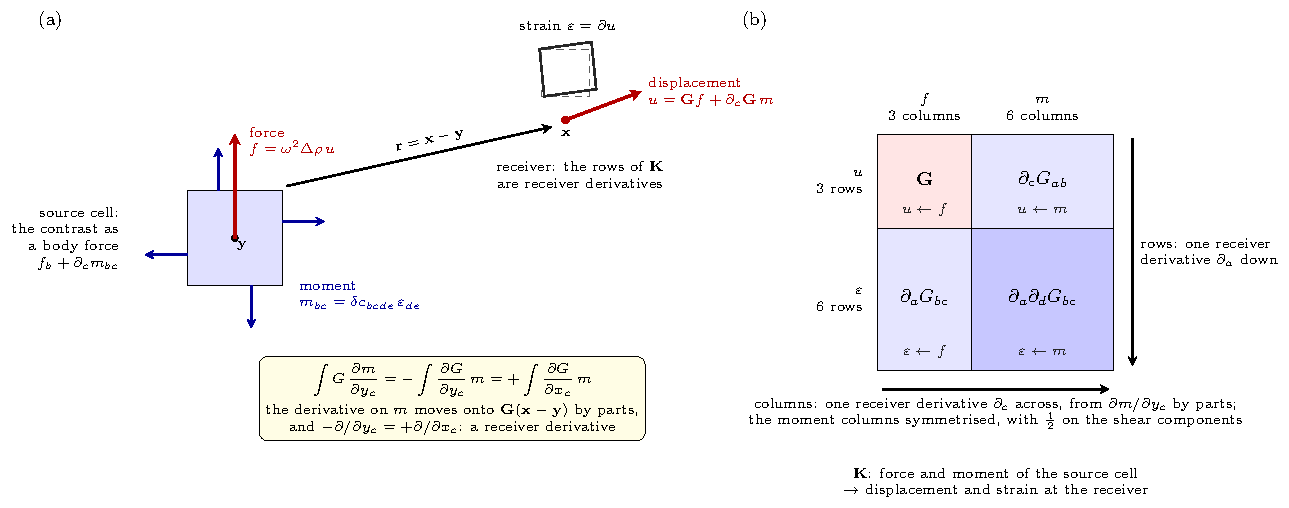
\includegraphics[width=\linewidth]{figures/fig_kernel.pdf}
\caption{Where the kernel comes from. (a) A source cell at $\mathbf y$ acts on the background through
the body force of Eq.~\eqref{eq:bodyforce}: a force $f$ from its density contrast, and the divergence
of its contrast stress $m$, the moment, from its stiffness contrast (arrows on the faces). At the
receiver $\mathbf x$ the state is the displacement $u$ and the strain $\varepsilon$. The moment's
derivative moves onto $\bG(\mathbf x-\mathbf y)$ by parts, Eq.~\eqref{eq:byparts}, and becomes a
receiver derivative with a plus sign. (b) The block structure of the $9\times9$ kernel $\bK$ that
results: the force columns are $\bG$, the moment columns carry one receiver derivative across, the
strain rows one receiver derivative down, and the strain-from-moment block two.}
\label{fig:kernel}
\par\smallskip{\footnotesize\textit{Alt text:} Two panels. On the left, a shaded square cell with a
dot at its centre marked y; a thick red arrow labelled force rises from the centre, and four blue
arrows labelled moment point outward from the cell's faces. A long arrow labelled r equals x minus y
runs from the cell to a red dot marked x at the upper right, from which a red arrow labelled
displacement leaves and above which a small dashed square deformed into a parallelogram is labelled
strain. A boxed line below reads: the integral of G times the y-derivative of m equals minus the
integral of the y-derivative of G times m, equals plus the integral of the x-derivative of G times m.
On the right, a two-by-two grid of shaded blocks with rows labelled u, three rows, and strain, six
rows, and columns labelled f, three columns, and m, six columns; the blocks read G, the first
derivative of G, the first derivative of G, and the second derivative of G; an arrow down the right
side reads rows: one receiver derivative down, and an arrow along the bottom reads columns: one
receiver derivative across.\par}
\end{figure}

\paragraph{Averaging, and collocation.} Three operations in this paper are averages over a cell,
and they are distinct. The \emph{source-cell average} integrates the kernel over the cell that
radiates: $\langle\bK\rangle(\mathbf r)=d^{-3}\int_{\text{cube}}\bK(\mathbf r-\mathbf y)\,\dd\mathbf y$
is the field at $\mathbf r$ of a uniform polarisation of the source cell. Every scheme in this paper
uses it, and \S\ref{sec:tiling} shows it to be exact. \emph{Collocation} fixes where the discrete
equation is imposed: at the receiving cell's centre, with the internal field of each cell uniform, so
that the unknown is the field at the centre. The \emph{receiver-cell average} imposes the equation in
the mean over the receiving cell instead; with a uniform internal field that is the Galerkin scheme
of degree zero, called the mean-only voxel below. The two are both \emph{uniform-field} voxels, a
term that refers to the internal field and not to the test, and they differ only in the test
function (a delta at the centre against the cell's indicator) and in the constant of their
$O((kd)^2)$ error (Table~\ref{tab:ratio}). The \emph{cell-mean contrast}, finally, is an average of
the material, not of the field: where the medium varies within a cell, the contrast is projected
onto the cell's basis, its mean for degree $r=0$, rather than sampled at the centre
(\S\S\ref{sec:hetero}, \ref{sec:sphere}). In the language of the coupled-dipole method, the point
dipole is collocation with the point kernel, the integrated Green tensor adds the source-cell
average, and the filtered coupled dipoles replace the point source by one of finite extent.

\paragraph{The laterally uniform layer.} A layer of thickness $D$ is filled with $n$ planes of
voxels, $d=D/n$, and illuminated at normal incidence. The field is then laterally uniform, only the
zero-lateral-wavenumber (specular) component of the lattice coupling acts, and
Eq.~\eqref{eq:foldylax} becomes exactly a chain of $n$ planes coupled by the specular lattice sums
\begin{equation}\label{eq:specsum}
  \bS(m)=\sum_{\mathbf R}\bG(\mathbf R+m d\,\hat{\mathbf z}),
\end{equation}
where the sum runs over the lattice vectors $\mathbf R=d\,(0,p,q)$, $p,q$ integers, that join the centres of
the voxels in one plane (a square lattice of pitch $d$), and $m$ is the separation of the two planes in
units of $d$ (Fig.~\ref{fig:lattice}a,b). The question is whether, and how fast, this chain converges to the
continuous layer as $n\to\infty$ at fixed $D$.

\begin{figure}[t]
\centering
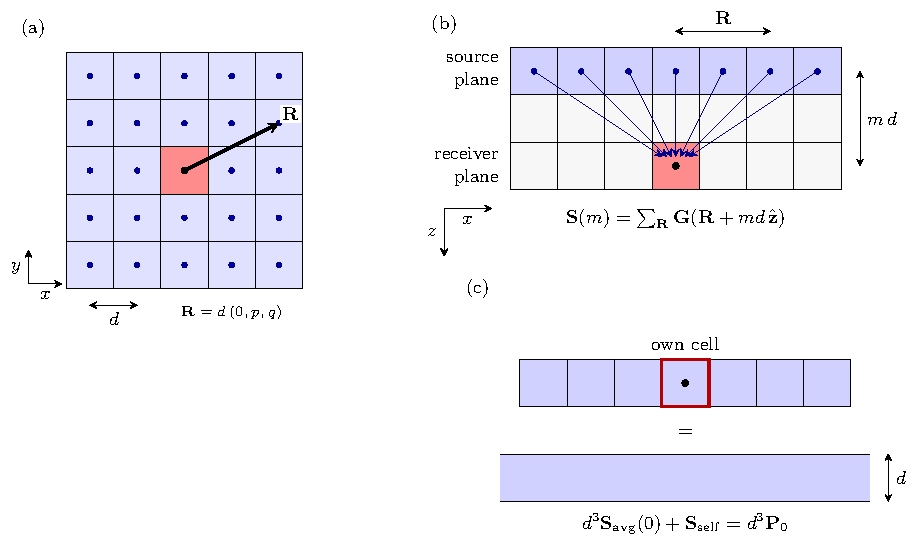
\includegraphics[width=\linewidth]{figures/fig_lattice.pdf}
\caption{The lattice and its sums. (a) Plan view of one plane of voxels: their centres form a square
lattice of pitch $d$, and a lattice vector $\mathbf R=d\,(0,p,q)$ joins the centre of one voxel (shaded darker)
to another. (b) Cross-section ($z$ down), between planes: the voxel of a receiver plane (shaded darker) is coupled
to every voxel of a source plane $m$ planes above it, one for each lattice vector $\mathbf R$; the sum
over $\mathbf R$ is the specular lattice sum of Eq.~\eqref{eq:specsum}. (c) Within a plane: the sum
over every cell of the plane, the receiver's own cell (outlined) included, is the field of a uniform
plate of thickness $d$, the tiling identity of Eq.~\eqref{eq:tiling}.}
\label{fig:lattice}
\par\smallskip{\footnotesize\textit{Alt text:} Three schematic panels. On the left, a plan view of a
five-by-five grid of square voxels with a dot at each centre; the centre voxel is highlighted, an arrow
labelled R runs from its centre to another voxel centre, and the spacing between neighbouring centres is
marked d. At the top right, a cross-section through three rows of voxels: arrows from the centre of every
voxel in the top row converge on a highlighted voxel two rows below, with the plane separation m d
marked. Below it, a single row of voxels with one outlined as the receiver's own cell is shown equal
to a continuous shaded band of the same thickness d, a uniform plate.\par}
\end{figure}

\paragraph{Implementations.} Every result is derived symbolically in Mathematica and compared with
an independent numerical implementation or an exact solution. ``The package'' below is the Python/Fortran
implementation of the voxel scheme (\path{cubic_scattering}): its cube $T$-matrix, its lattice
kernels and its stratified propagator, which serve both as the object under test and, where
validated, as a second implementation.


\section{The continuous layer and its thin-layer expansion}\label{sec:continuum}

At normal incidence a plane force drives a one-dimensional problem per wave type, with modulus $M$
($M_P$ for P, $\mu$ for S), wavenumber $k$ and plane Green's function
$g(z)=\tfrac{\mathrm{i}}{2Mk}\mathrm{e}^{\mathrm{i}k|z|}$. The layer's reflection and transmission follow from continuity of
displacement and traction at its faces; they agree with the stratified propagator used as the
reference in this work to $2.5\times10^{-8}$, P and S (\nb{ContinuumLimit\_Reference.wl}).

For a layer of thickness $D$ with modulus $M_1$ and density $\rho_1$ in a background $M_0,\rho_0$,
write $Z_j=\sqrt{M_j\rho_j}$ for the impedances, $\zeta=Z_1/Z_0$ for their ratio and
$k_1=\omega\sqrt{\rho_1/M_1}$ for the layer's wavenumber. The reflection coefficient expands as
\begin{equation}\label{eq:thin}
\begin{aligned}
  R={}&\frac{\mathrm{i}k_1D}{2}\bigl(\zeta-\zeta^{-1}\bigr)
  +\frac{(k_1D)^2}{4}\bigl(\zeta^{-2}-\zeta^{2}\bigr)
  -\frac{\mathrm{i}(k_1D)^3}{24}\bigl(\zeta-\zeta^{-1}\bigr)\bigl(3\zeta^{-2}+2+3\zeta^{2}\bigr)\\
  &+\frac{(k_1D)^4}{48}\bigl(\zeta^{2}-\zeta^{-2}\bigr)\bigl(3\zeta^{2}-2+3\zeta^{-2}\bigr)+O(D^5),
\end{aligned}
\end{equation}
exact in the contrast (\nb{ContinuumLimit\_ThinLayer.wl}, which checks each coefficient symbolically
and the truncated series against the exact layer). The first term is
\begin{equation}\label{eq:thin1}
  \frac{\mathrm{i}\omega D}{2}\sqrt{\frac{M_0}{\rho_0}}
  \Bigl[\frac{\rho_1-\rho_0}{M_0}-\rho_0\Bigl(\frac1{M_1}-\frac1{M_0}\Bigr)\Bigr]:
\end{equation}
to first order a thin layer is an
interface across which the traction jumps by the excess inertia and the displacement by the excess
compliance. At oblique incidence the same statement holds with the first-order system
$\partial_z\mathbf b=\bA\mathbf b$ for the P--SV state $\mathbf b=(u_x,u_z,t_{xz},t_{zz})$: the layer
acts to $O(D)$ as the jump $\bI+(\bA_1-\bA_0)D$, which reproduces the layer's $O(D)$ reflection
coefficients $R_{PP},R_{PS}$ to $10^{-12}$; the series truncated at $O(D^k)$ converges at exactly
order $k$; and a soft thin layer with shear modulus $\mu_1=D/\eta$ at fixed compliance $\eta$ tends to
the linear-slip interface as $D\to0$. These expansions are the target a single plane of voxels must
reproduce order by order. A plane of voxels that carry Legendre moments of their internal field to
degree $p$ reproduces Eq.~\eqref{eq:thin} term by term through $O(D^{2p+2})$ and first differs at
$D^{2p+3}$ (\S\ref{sec:fourth}): the mean-only voxel reproduces the equivalent interface and the $D^2$
term, the first-moment voxel all four terms shown.

\section{The specular sums of the point Green's tensor}\label{sec:point}

\paragraph{Why transform the sum.} The specular sum \eqref{eq:specsum} adds, at a receiver, the field
of every voxel of a plane $m$ planes away. In that form it is a poor object to study. The Green's
tensor decays slowly with distance, so the sum converges slowly, and it hides the one question that
matters here: which part of it is the continuum, and which part is the discretisation. The Poisson
summation formula \citep{SteinWeiss1971} answers both at once, and is the standard tool for lattice sums
of wave fields \citep{Linton2010}. For a function $f$ on the plane and the square lattice of pitch $d$
it states
\begin{equation}\label{eq:poissonformula}
  \sum_{\mathbf R}f(\mathbf R)=\frac1{d^2}\sum_{\mathbf g}\hat f(\mathbf g),\qquad
  \hat f(\mathbf g)=\int f(\mathbf x)\,\mathrm{e}^{-\mathrm{i}\mathbf g\cdot\mathbf x}\,\dd^2x,\qquad
  \mathbf g=\tfrac{2\pi}{d}(p,q),
\end{equation}
with $p,q$ integers: a sum of samples of $f$ on the lattice equals a sum of samples of its Fourier
transform on the reciprocal lattice, whose pitch is $2\pi/d$ (Fig.~\ref{fig:poisson}). Applied to the
specular sum,
\begin{equation}\label{eq:poisson}
  \bS(m)=\frac1{d^2}\sum_{\mathbf g}\hat\bG(\mathbf g;\,m d),
\end{equation}
with $\hat\bG(\mathbf g;z)$ the two-dimensional (lateral) transform of the Green's tensor between planes
a distance $z$ apart. Each term has a physical meaning. Transformed laterally, the field of a plane of
sources is a superposition of plane waves, one for each lateral wavenumber, and the lattice selects the
wavenumbers $\mathbf g$. The order $\mathbf g=0$ is the laterally uniform plane wave that a continuous
layer radiates: it is the continuum's term. Every other order has $|\mathbf g|\ge2\pi/d$, far beyond the
wavenumber of the field when the voxels are small compared with the wavelength, so it is evanescent and
decays away from the plane as $\mathrm{e}^{-|\mathbf g|md}=\mathrm{e}^{-2\pi m\sqrt{p^2+q^2}}$, independently
of $d$. The transform therefore splits the lattice sum exactly into the continuum and a discretisation
correction, and the correction converges after a few orders.

\begin{figure}[t]
\centering
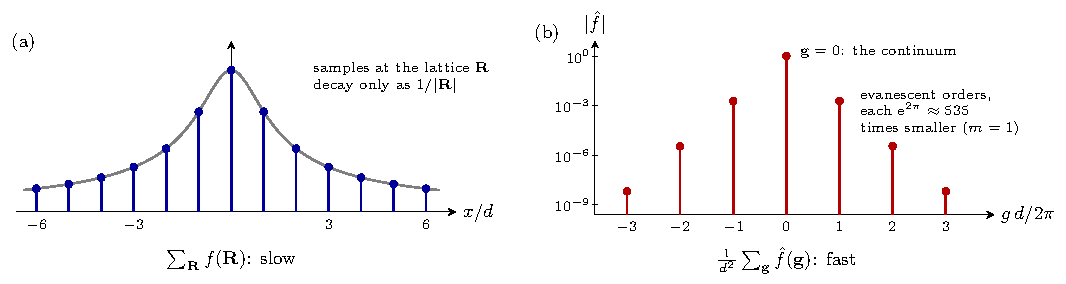
\includegraphics[width=\linewidth]{figures/fig_poisson.pdf}
\caption{The Poisson summation formula \eqref{eq:poissonformula} applied to a plane of voxels, along one
lateral axis. (a) Real space: the field of each voxel of a source plane at a receiver one plane away,
sampled at the lattice points; the samples decay only as $1/|\mathbf R|$, so their sum converges
slowly. (b) The same sum after Poisson summation, on a logarithmic scale: samples of the lateral Fourier
transform at the reciprocal-lattice orders $\mathbf g=2\pi p/d$. The order $\mathbf g=0$ is the
continuum's plane wave; every other order is evanescent and, at $m=1$, smaller than its neighbour by
$\mathrm{e}^{2\pi}\approx535$. Magnitudes are schematic: the static decay $\mathrm{e}^{-|\mathbf g|md}$ is
shown.}
\label{fig:poisson}
\par\smallskip{\footnotesize\textit{Alt text:} Two panels. On the left, a smooth bell-shaped curve that
decays slowly on both sides is sampled by vertical stems at integer positions from minus six to six,
the stems remaining clearly visible far from the centre. On the right, on a logarithmic vertical axis
from one down to ten to the minus nine, a stem of height one at zero is labelled as the continuum, and
stems at plus and minus one, two and three fall by about three powers of ten per step and are labelled
as evanescent orders.\par}
\end{figure}

\paragraph{The local term that survives.} In the strain-from-moment block the evanescent orders carry two
powers of $|\mathbf g|\propto1/d$, so their contribution per voxel volume does \emph{not} vanish as
$d\to0$: at $m=1$ it is eleven times the continuum term (\nb{ContinuumLimit\_SpecularSums.wl},
matched to the package's Ewald lattice sum to $5\times10^{-13}$). This surviving term is static.
Summed over all planes in slab order, the static lattice sum of the point kernel is exactly the
depolarisation of a uniform plate ($-1/M_P$ on $\varepsilon_{zz}\leftarrow M_{zz}$ and $-1/(2\mu)$
on the normal shears, per unit volume) plus a cubic-symmetric remainder
(\nb{ContinuumLimit\_StaticLocal.wl}, to $2\times10^{-10}$). The point kernel therefore reproduces
the continuum only if that remainder is cancelled by the voxel's own self term.

\section{The tiling identity}\label{sec:tiling}

Replace the point coupling by the \emph{source-cell average}
$\langle\bG\rangle(\mathbf r)=d^{-3}\int_{\text{cube}}\bG(\mathbf r-\mathbf y)\,\dd\mathbf y$, the
field at a voxel centre of a uniform polarisation of the source voxel. Each Poisson order in
Eq.~\eqref{eq:poisson} is then multiplied by the cube's form factor
\begin{equation}
  F(\mathbf g)=\sinc(g_x h)\,\sinc(g_y h),
\end{equation}
which vanishes at every $\mathbf g\neq0$ of the reciprocal lattice since $\sinc(p\pi)=0$ for integer
$p\neq0$. This is the Fourier form of the fact that cubes tile the plane,
$\sum_{\mathbf R}\chi(\mathbf x-\mathbf R)=1$ for the cube's indicator $\chi$: a partition of unity
(Fig.~\ref{fig:tiling}). Two exact statements follow.

\begin{figure}[t]
\centering
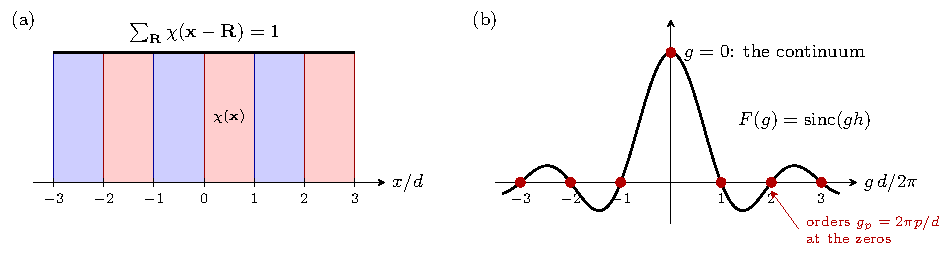
\includegraphics[width=\linewidth]{figures/fig_tiling.pdf}
\caption{Why cubes make the coupling exact. (a) Cubes tile the plane: the indicator functions $\chi$ of
the translated cells sum to exactly one everywhere, a partition of unity. (b) The same fact in Fourier
space: the cube's lateral form factor $F(g)=\sinc(gh)$ (shown along one axis) vanishes at every
reciprocal-lattice order $g_p=2\pi p/d$ with $p\neq0$, so of all the orders in the lattice sum
\eqref{eq:poisson} only $g=0$, the continuum's plane wave, survives the source-cell average.}
\label{fig:tiling}
\par\smallskip{\footnotesize\textit{Alt text:} Two panels. On the left, adjacent box functions of unit
height and unit width, alternately shaded, lie side by side along an axis marked in voxel widths, and a
thick horizontal line at height one marks their sum. On the right, the sinc curve, equal to one at the
origin and oscillating with decaying amplitude, is plotted against wavenumber in units of $2\pi/d$; dots
mark the reciprocal-lattice orders, one at height one at the origin and all the others on the axis at
the zeros of the curve.\par}
\end{figure}

\paragraph{Between planes.} For $m\neq0$ every evanescent order is removed and
\begin{equation}\label{eq:between}
  \bS_{\text{avg}}(m)=\frac1{d^2}\sum_{W=P,S}\hat\bG_W(0;\,m d)\,\sinc(k_W h),
\end{equation}
the continuum's plane-wave term times the vertical form factor. The package's cell-averaged kernel
agrees in all 81 entries to $2.8\times10^{-16}$ (\nb{ContinuumLimit\_AveragedSums.wl}).

\paragraph{Within a plane.} The sum over \emph{all} cells of the plane, the voxel's own included,
is the field at the mid-plane of a uniform plate of thickness $d$ (Fig.~\ref{fig:lattice}c):
\begin{equation}\label{eq:tiling}
  d^3\,\bS_{\text{avg}}(0)+\bS_{\text{self}}=d^3\,\bP_0,
  \qquad
  \bS_{\text{self}}=\int_{\text{cube}}\bG(-\mathbf y)\,\dd\mathbf y,
\end{equation}
where $\bP_0=d^{-3}\int_{-h}^{h}\bG_{\text{plate}}(-z')\,\dd z'$ is elementary: in the one-dimensional
transform each entry is $c_0+A/(Mk_z^2-\rho\omega^2)$, so it averages to
$c_0/d+A\,(\mathrm{e}^{\mathrm{i}kh}-1)/(dMk^2)$. Its only nonzero entries are $u\leftarrow f$ on the diagonal and the
three normal strain-from-moment entries, whose local weights $-1/M_P$ and $-1/(2\mu)$ are the plate
depolarisation of \S\ref{sec:point}. Statically the identity holds for all 21 independent components
of the strain-from-moment tensor to $4\times10^{-9}$, with every cell integral evaluated analytically
(below).

\paragraph{Consequence: an exact kernel with no lattice sum.} At normal incidence the same-plane
block of the cell-averaged Foldy--Lax kernel is
\begin{equation}\label{eq:exactkernel}
  \bS_{\text{avg}}(0)=\bP_0-\bS_{\text{self}}/d^3 ,
\end{equation}
with no Ewald splitting, near shell or asymptotic tail. The route it replaces (Ewald summation
with a near shell averaged by quadrature and an $O(d^2)$ Taylor tail beyond it) carries a static
strain-from-moment error of $9.4\times10^{-4}$ at its default settings, falling to $2.6\times10^{-5}$
only when both the shell radius and the quadrature order are raised; Eq.~\eqref{eq:exactkernel} is
now the package's kernel at normal incidence.

\paragraph{Cell integrals without quadrature.} Write the static (Kelvin) tensor as
$G_{bc}=(c_A+c_B)\,\delta_{bc}/r-c_B\,\partial_b\partial_c r$ with
$c_B=(1/\mu-1/M_P)/8\pi$ and $c_A=1/(4\pi\mu)-c_B$. Every cell integral of its derivatives is a cell
integral of derivatives of $1/r$ and $r$. One application of the divergence theorem moves it onto
faces $x_p=c_p\pm h$, which never contain the origin, and there the two-dimensional antiderivative in
the face coordinates is continuous, so the face integral is a sum over the face's corners. The
distributional term at $r=0$ is carried by the divergence theorem itself. (A triple antiderivative
evaluated at the cube's corners is \emph{not} usable for repeated derivatives: its arctangent terms
jump across the coordinate planes through the origin, and differentiating twice there discards
exactly that term.) The self term so obtained reproduces the classical closed form of the cube's
depolarisation \citep{Chiu1977,Nozaki2001} to machine precision.


\paragraph{The collocation scheme.} The simplest voxel takes its internal field as uniform. Its
single-site $T$-matrix is then the uniform-strain closure $\bT=d^3\,\bD\bigl(\bI-\bS_{\text{self}}\bD\bigr)^{-1}$,
with $\bS_{\text{self}}$ the nine-component self term of the cube, whose moments of the Green's tensor are
in closed form \citep{NestorContinuum2026}; for internal state $e$ the voxel's own field at its centre is
$\bS_{\text{self}}\bD\,e$, and $e=\psi+\bS_{\text{self}}\bD e$.
With the kernel \eqref{eq:exactkernel} the self term cancels. Substituting
$\psi=(\bI-\bS_{\text{self}}\bD)e$ into Eq.~\eqref{eq:foldylax},
\begin{equation}\label{eq:collocation}
  e_i=\psi^0_i+d^3\sum_j \bK_{\text{all}}(i,j)\,\bD\,e_j,
  \qquad
  \bK_{\text{all}}(i,i)=\bP_0,\quad \bK_{\text{all}}(i,j)=\bS_{\text{avg}}(i-j),
\end{equation}
an identity checked on the matrices to $4\times10^{-16}$. Every block of $\bK_{\text{all}}$ is an
\emph{exact} cell integral of the one-dimensional continuum kernel (Eqs.~\eqref{eq:between},
\eqref{eq:tiling}), so Eq.~\eqref{eq:collocation} is precisely the collocation of the continuum
Lippmann--Schwinger equation with a strain piecewise constant over voxels. It does not contain
$\bS_{\text{self}}$ at all.

The package's cube $T$-matrix is this closure statically, to $2\times10^{-5}$ at $k_Sh=0.01$, and departs
dynamically by about $0.25(kh)^2$ through its far-field form-factor corrections
\citep{NestorContinuum2026}; by Eq.~\eqref{eq:collocation} that departure cannot enter the closure scheme.

\section{Convergence, and the closed-form error}\label{sec:convergence}

\paragraph{The experiment.} Every convergence test of this paper is the same experiment, varied in one
respect at a time, and it is set out here once.
\begin{enumerate}
\item \emph{The medium.} The background has $\alpha=5000$ and $\beta=3000$\,m\,s$^{-1}$ and
$\rho=2500$\,kg\,m$^{-3}$. The layer occupies $0<z<D$ with $D=2$\,m, and differs from the background by
$\Delta\lambda=2$\,GPa, $\Delta\mu=1$\,GPa and $\Delta\rho=100$\,kg\,m$^{-3}$: $6.4\%$ in the P modulus,
$4.4\%$ in the shear modulus and $4\%$ in the density.
\item \emph{The source.} A plane force at $z_s=-12$\,m, above the layer, radiates a plane wave towards
it. The incident field in the layer is then known in closed form, and it is smooth there because the
source is outside.
\item \emph{What is measured.} The scattered displacement, total less incident, at two observers
outside the layer: at $z=-1$\,m above it, where it is the reflected wave, and at $z=4$\,m below it,
where it is the change the layer makes to the transmitted wave. Outside the layer the scattered field
is a single outgoing wave, so one observer on each side holds everything; the two are reported
separately, as reflection / transmission.
\item \emph{The exact answer.} The reflection and transmission of the layer from continuity of
displacement and traction at its two faces (\S\ref{sec:continuum}); for a layer whose properties vary
with depth, from the differential equation integrated to $30$ digits.
\item \emph{The error.} $e=\lvert u_{\text{scheme}}-u_{\text{exact}}\rvert/\lvert u_{\text{exact}}\rvert$
at each observer: relative to the scattered field, not to the total, so that an error of $10^{-6}$ is a
millionth of what the layer scatters.
\item \emph{The refinement.} The layer is cut into $n$ planes of voxels of side $d=D/n$, with $n$ from
$1$ to $32$, at $\omega=60$, $300$ and $600$\,rad\,s$^{-1}$, for which $k_PD=0.024$, $0.12$ and $0.24$
and $k_SD=0.04$, $0.2$ and $0.4$. Three frequencies show that an order is not an accident of one.
\item \emph{The arithmetic.} The errors of the higher-degree voxels fall below the round-off of double
precision, so the symbolic implementation computes them to $40$ digits; the independent numerical
implementation, in double precision, agrees with it down to its own floor of about $10^{-13}$.
\end{enumerate}
The later sections change one item each: the incident wave to SV or SH and its angle
(\S\ref{sec:fourth}), the medium to a stratified or a graded one and the background to a stratified one
(\S\ref{sec:hetero}), and the body to a sphere (\S\ref{sec:sphere}).

\paragraph{Second order.} For a layer $D=2$\,m with the contrast
$\Delta\lambda=2$\,GPa, $\Delta\mu=1$\,GPa, $\Delta\rho=100$\,kg\,m$^{-3}$ in a background
$\alpha=5000$, $\beta=3000$\,m\,s$^{-1}$, $\rho=2500$\,kg\,m$^{-3}$, illuminated by a P plane force,
the reflected displacement of the chain converges to the continuous layer's at order $2.000$ for
$n=4\to16$ at $\omega=60$, $300$ and $600$\,rad\,s$^{-1}$, with the collocation
\eqref{eq:collocation} and with the package $T$-matrix alike (\nb{ContinuumLimit\_Chain.wl}). The
error depends on $k_Sh$ alone. Throughout, an order quoted for a pair of grids is the apparent order
$\ln(e_1/e_2)/\ln(n_2/n_1)$ between them, with $e$ the relative error against the exact solution
and $n$ the refinement; the orders in the legend of Fig.~\ref{fig:convergence} are least-squares
slopes of $\ln e$ against $\ln n$ over the grids marked as fitted, with their standard errors. The
two agree where a sequence is asymptotic and differ where it is not, which the apparent orders show.

\paragraph{The leading error in closed form.} In Eq.~\eqref{eq:collocation} the kernel is
integrated exactly; the only approximation is the internal field's variation across a voxel. At
first order in the contrast the discrete scattered field is therefore a midpoint rule applied to
the continuum's Born integral, with the kernel's cell integral exact. For reflection the integrand
carries the two-way phase $\mathrm{e}^{2\mathrm{i}kz}$; for transmission it is flat. With $k$ the background
wavenumber of the wave concerned ($k_P$ for an incident P wave, $k_S$ for an incident S wave), $R$ the reflection coefficient and $T^{\text{sc}}$ the
scattered part of the transmitted field, for \emph{every} $n$
\begin{equation}\label{eq:errorR}
  \frac{R_{\text{disc}}}{R}=\frac{\sinc(kh)}{\sinc(2kh)}=1+\frac{(kd)^2}{8}+O(d^4),
  \qquad
  \frac{T^{\text{sc}}_{\text{disc}}}{T^{\text{sc}}}=\sinc(kh)=1-\frac{(kd)^2}{24}+O(d^4),
\end{equation}
confirmed for $n=1$ to $16$ to $10^{-4}$ of the error itself
(\nb{ContinuumLimit\_ErrorConstant.wl}); for an incident S wave, with $k=k_S$, the same forms and those of
Eq.~\eqref{eq:ratio} hold to $4\times10^{-4}$ (\nb{ContinuumLimit\_IncidentS.wl}, \S\ref{sec:fourth}). At the full contrast the reflection constant is unchanged
($0.124$ against $1/8$); the transmission constant grows to $-0.092$.

\paragraph{Why a uniform-field single site stops at second order.} The two constants have opposite
signs, so no scalar correction of $\bT$, no single $O((kh)^2)$ factor, can cancel both. The
package $T$-matrix illustrates it: its form-factor corrections reduce the reflection error by a
factor $4.45$ and \emph{increase} the transmission error by $1.7$, at every $n$. The missing term in
Eq.~\eqref{eq:errorR} is the first moment of the internal field over each voxel, which radiates
through the derivative of the kernel. A fourth-order scheme must carry it: a single site with a
gradient channel, and a kernel whose cell integrals include the kernel's derivative.

\section{Fourth order and beyond: Legendre moments of the voxel field}\label{sec:fourth}

Let each voxel carry the mean \emph{and} the first moment of its internal field. On voxel $j$, with
local coordinate $s\in[-h,h]$ and Legendre functions $\phi_b(s)=P_b(s/h)$ ($\phi_0=1$, $\phi_1=s/h$,
$\phi_2=(3s^2/h^2-1)/2$, \dots), the field is
$w=\sum_{b}c_{b,j}\,\phi_b$, $w=(u,\varepsilon)$ the displacement and strain of the P channel, and
the polarisation is $q=(\omega^2\Delta\rho\,u,\ \Delta M\,\varepsilon)$ with $\Delta M=\Delta\lambda
+2\Delta\mu$. Testing the continuum equation
\begin{equation}
  w(z)=w^0(z)+\int\bK(z-z')\,q(z')\,\dd z',\qquad
  \bK=\begin{pmatrix} g & g' \\ g' & g''\end{pmatrix},\quad g''=-k^2g-\delta(z)/M_P,
\end{equation}
with the same functions on every voxel gives
\begin{equation}\label{eq:galerkin}
  \Bigl(\int_{i}\phi_a^2\,\dd z\Bigr)c_{a,i}
  =\int_i\phi_a w^0\,\dd z+\sum_{j,b}\Bigl[\int_i\!\!\int_j\phi_a(z)\,\bK(z-z')\,\phi_b(z')\,\dd z\,\dd z'\Bigr]
  \bD_1 c_{b,j},
\end{equation}
$\bD_1=\operatorname{diag}(\omega^2\Delta\rho,\Delta M)$. Between voxels the double integral is
separable, a product of Legendre moments of $\mathrm{e}^{\pm \mathrm{i}kz}$; within a voxel it is split at $z'=z$ and
the local term contributes $-\int_i\phi_a\phi_b\,\dd z/M_P$. Every entry is closed-form. Keeping only
$\phi_0$ recovers a second-order scheme; keeping $\phi_0$ and $\phi_1$ converges at fourth order in
both reflection and transmission (\nb{ContinuumLimit\_FourthOrder.wl}; Table~\ref{tab:fourth1d}).
\begin{table}[htbp]
\centering
\caption{Relative error of the scattered displacement of the layer, reflection / transmission, at $\omega=300$\,rad\,s$^{-1}$, against the number of voxel planes $n$: collocation, the mean-only voxel and the first-moment voxel of Eq.~\eqref{eq:galerkin}. The order is $4.00$ at $\omega=60$ and $600$\,rad\,s$^{-1}$ too.}\label{tab:fourth1d}
\begin{tabular}{@{}rccc@{}}
\toprule
$n$ & collocation & mean only & mean and first moment \\
\midrule
$1$  & $1.8\times10^{-3}$ / $1.3\times10^{-3}$ & $1.2\times10^{-3}$ / $1.8\times10^{-3}$ &
       $2.8\times10^{-7}$ / $2.8\times10^{-7}$ \\
$4$  & $1.1\times10^{-4}$ / $8.3\times10^{-5}$ & $7.5\times10^{-5}$ / $1.1\times10^{-4}$ &
       $1.1\times10^{-9}$ / $1.1\times10^{-9}$ \\
$16$ & $7.0\times10^{-6}$ / $5.2\times10^{-6}$ & $4.7\times10^{-6}$ / $6.9\times10^{-6}$ &
       $4.2\times10^{-12}$ / $4.2\times10^{-12}$ \\
order & $2$ / $2$ & $2$ / $2$ & $4$ / $4$ \\
\bottomrule
\end{tabular}
\end{table}
A single plane of first-moment
voxels represents the $2$\,m layer $6500$ times more accurately than a single plane of uniform ones.
The collocation column is the scheme of Eq.~\eqref{eq:collocation} and reproduces the chain of the full
$9\times9$ system to all printed digits.

\paragraph{Higher moments.} Carrying the Legendre moments to degree $p$ changes nothing in the
construction: the moments and the same-cell double integrals of $P_b(s/h)$ against exponentials are
again closed-form, and for $p\le1$ the general-degree solver reproduces the chain above exactly. The
second-moment voxel ($p=2$) converges at sixth order and the third-moment voxel ($p=3$) at eighth, in
reflection and transmission (Table~\ref{tab:layerhigher}; \nb{ContinuumLimit\_SecondMoment.wl}); the
second-moment voxel's order is $6.00$ at $\omega=60$, $300$ and $600$\,rad\,s$^{-1}$. The errors fall to
$10^{-22}$, so they are computed in 40-digit arithmetic.
\begin{table}[htbp]
\centering
\caption{Relative error of the scattered displacement of the layer, reflection / transmission, at
$\omega=300$\,rad\,s$^{-1}$, for voxels carrying Legendre moments to degree $p$. The order is the mean
over the halvings $n=2\to4\to8$.}\label{tab:layerhigher}
\small\setlength{\tabcolsep}{4pt}
\begin{tabular}{@{}rccc@{}}
\toprule
$n$ & first moment ($p=1$) & second moment ($p=2$) & third moment ($p=3$) \\
\midrule
$1$ & $2.8\times10^{-7}$ / $2.8\times10^{-7}$ & $2.8\times10^{-11}$ / $4.2\times10^{-11}$ &
      $1.5\times10^{-15}$ / $1.5\times10^{-15}$ \\
$2$ & $1.7\times10^{-8}$ / $1.7\times10^{-8}$ & $4.4\times10^{-13}$ / $6.5\times10^{-13}$ &
      $6.0\times10^{-18}$ / $6.0\times10^{-18}$ \\
$4$ & $1.1\times10^{-9}$ / $1.1\times10^{-9}$ & $6.9\times10^{-15}$ / $1.0\times10^{-14}$ &
      $2.4\times10^{-20}$ / $2.4\times10^{-20}$ \\
$8$ & $6.7\times10^{-11}$ / $6.7\times10^{-11}$ & $1.1\times10^{-16}$ / $1.6\times10^{-16}$ &
      $9.2\times10^{-23}$ / $9.2\times10^{-23}$ \\
order & $4$ / $4$ & $6$ / $6$ & $8$ / $8$ \\
\bottomrule
\end{tabular}
\end{table}

\paragraph{The leading error in closed form.} Without scattering, the Galerkin solution is the
$L^2$ projection $\Pi$ of the incident field onto each voxel's basis, and the kernel is integrated
over each voxel exactly; at first order in the contrast the error is therefore the kernel's cell
integral applied to $\Pi w^0-w^0$. The field varies as $\mathrm{e}^{\mathrm{i}ks}$ across a voxel and the kernel toward
an outside observer as $\mathrm{e}^{\mathrm{i}qs}$, $q=+k$ for reflection and $q=-k$ for transmission, so for every
scheme and every $n$
\begin{equation}\label{eq:ratio}
  \frac{\text{discrete}}{\text{exact}}
  =\frac{\int_{-h}^{h}\mathrm{e}^{\mathrm{i}qs}\,\Pi[\mathrm{e}^{\mathrm{i}ks}]\,\dd s}{\int_{-h}^{h}\mathrm{e}^{\mathrm{i}(q+k)s}\,\dd s},
\end{equation}
with $\Pi$ the centre value for collocation, the cell mean for the mean-only voxel and the projection
onto $\{P_0,\dots,P_p\}$ for the voxel of degree $p$ (\nb{ContinuumLimit\_FourthOrderError.wl},
\nb{ContinuumLimit\_SecondMoment.wl}). The results are in Table~\ref{tab:ratio}.
\begin{table}[htbp]
\centering
\caption{The leading error of the discrete layer in closed form, Eq.~\eqref{eq:ratio}: discrete over exact scattered field at first order in the contrast, for every number of voxel planes $n$.}\label{tab:ratio}
\begin{tabular}{@{}lcc@{}}
\toprule
 & reflection & transmission \\
\midrule
collocation      & $1+(kd)^2/8+O(d^4)$  & $1-(kd)^2/24+O(d^4)$ \\
mean only        & $1+(kd)^2/12+O(d^4)$ & $1-(kd)^2/12+O(d^4)$ \\
first moment     & $1-(kd)^4/720+O(d^6)$ & $1-(kd)^4/720+O(d^6)$ \\
second moment    & $1+(kd)^6/100800+O(d^8)$ & $1-(kd)^6/100800+O(d^8)$ \\
third moment     & $1-(kd)^8/25401600+O(d^{10})$ & $1-(kd)^8/25401600+O(d^{10})$ \\
degree $p$       & $1+(-1)^pc_p(kd)^{2p+2}$ & $1-c_p(kd)^{2p+2}$ \\
\bottomrule
\end{tabular}
\end{table}
The chain of Eq.~\eqref{eq:galerkin} reproduces the forms for collocation and degrees $0$ and $1$
at $n=1$ to $8$ to $10^{-4}$ of the error, the remainder being the second order in the contrast, and
those for degrees $2$ and $3$ to $4\times10^{-7}$ at a contrast reduced by $10^{-6}$. The constant for
degree $p$ follows from the Legendre expansion
$\mathrm{e}^{\mathrm{i}ks}=\sum_j\mathrm{i}^j(2j+1)\,j_j(kh)\,P_j(s/h)$. The projection drops the terms
$j>p$, led by $j=p+1$, whose coefficient is $O\bigl((kh)^{p+1}\bigr)$; its moment against
$\mathrm{e}^{\mathrm{i}qs}$ is $2h\,\mathrm{i}^{p+1}j_{p+1}(qh)=O\bigl((qh)^{p+1}\bigr)$. With
$j_n(x)\approx x^n/(2n+1)!!$ and $h=d/2$,
\begin{equation}\label{eq:cp}
  c_p=\frac{2p+3}{4^{p+1}\bigl[(2p+3)!!\bigr]^2}=\frac{\bigl[(p+1)!\bigr]^2}{(2p+2)!\,(2p+3)!},
  \qquad c_0=\tfrac1{12},\ c_1=\tfrac1{720},\ c_2=\tfrac1{100800},
\end{equation}
and the leading error carries $(q/k)^{p+1}$: the same sign in reflection and transmission for odd
$p$, opposite signs for even $p$. The first-moment voxel's leading error therefore does not depend on
the direction in which the field is observed. Eq.~\eqref{eq:cp} is checked symbolically for $p=0$ to
$5$ (every lower power of $kd$ vanishes) in Mathematica and, independently, in sympy.

\paragraph{One plane of voxels and the thin-layer series.} Refining at fixed thickness is one limit;
thinning a single plane is the other. For one plane of voxels ($n=1$, $d=D$) the series in $D$ of the
reflection coefficient, computed exactly at the full contrast, coincides with that of the exact layer,
Eq.~\eqref{eq:thin}, term by term through $D^{2p+2}$ and first differs at $D^{2p+3}$, for $p=0$ to $3$
and for a layer both stiffer and softer than its surroundings (\nb{ContinuumLimit\_SecondMoment.wl}).
Each further Legendre moment adds two terms of the thin-layer series.

\paragraph{In three dimensions.} The three-dimensional first-moment voxel carries the nine-component
state with Legendre weights $\{1,\,x/h,\,y/h,\,z/h\}$, 36 unknowns in all, tested with the same
functions and coupled by cell-to-cell double integrals of the Green's tensor. For a laterally uniform
layer at normal incidence it reduces \emph{exactly} to Eq.~\eqref{eq:galerkin}
(\nb{ContinuumLimit\_Reduction3D.wl}). The lateral first moments are never excited: the lattice and
the incident field are symmetric under reflection about every voxel's centre planes, and $x/h$, $y/h$
are odd there. The mean and the $z$-moment carry weights that are constant laterally, so their lateral
form factor $\sinc(g_xh)\sinc(g_yh)$ vanishes on the reciprocal lattice and the plane sum of the
double integrals is the plate-to-plate integral in $z$ alone. Two facts mark where genuinely
three-dimensional structure begins. The lateral first moment's form factor,
$F_1(g)=\mathrm{i}\,(gh\cos gh-\sin gh)/(gh)^2$, does not vanish on the reciprocal lattice
($F_1=\mathrm{i}(-1)^p/p\pi$), so the gradient channels couple through the evanescent orders. And at oblique
incidence the mean's own zeros shift, $\sinc\bigl((2\pi p/d+k_x)h\bigr)=(-1)^p k_xh/p\pi+O(k_x^2h^2)$,
so the tiling identity holds only to $O(k_\parallel h)$.

\paragraph{Other angles, other waves, and degree two.} The orders and their constants hold beyond
normal incidence and incident P. At oblique incidence, where the tiling identity holds only to
$O(k_\parallel h)$ and the gradient channels couple through the evanescent orders, the mean-only and
first-moment voxels remain second and fourth order in the reflected P and the converted S wave; for
incident SV and SH waves the orders, and with $k=k_S$ the constants, are those of incident P; and the
voxel of degree two converges at sixth order for P, SV and SH waves, its error on four planes at normal
incidence being the $c_2(kd)^6$ of Eq.~\eqref{eq:cp} to $4\%$. Appendix~\ref{app:legendre} gives the
spectral construction, Eq.~\eqref{eq:bloch}, the tests, and the second implementations that check
them; Figure~\ref{fig:convergence}(a,b) shows the convergence.


\FloatBarrier
\section{A heterogeneous layer}\label{sec:hetero}

A heterogeneous medium is not a layer of identical cells. The simplest heterogeneous case with an
exact answer is a stratified model built from layers of constant properties, with real interfaces
between them: the form of many layered crustal velocity models. The last test takes such a model. A
layer $D=4$\,m thick is divided into eight model layers of $0.5$\,m, and in each one $\Delta\lambda$, $\Delta\mu$
and $\Delta\rho$ are drawn uniformly within $\pm15\%$ of the background (the values are listed in
\nb{ContinuumLimit\_Heterogeneous.wl}). The result is a random stratification with physical contrasts. The voxels refine
the model's layering, with $m$ planes of voxels in each model layer, so no voxel straddles a model
interface: the natural discretisation when the model's interfaces are known. At $\omega=1500$\,rad\,s$^{-1}$ the layer is
$k_PD=1.2$ and $k_SD=2.0$ thick, so the field reverberates between the model interfaces. The schemes are those of \S\S\ref{sec:convergence}--\ref{sec:fourth}, with the
contrast now changing from plane to plane; nothing else in them changes. In the terms of the
experiment of \S\ref{sec:convergence}, the test is this.
\begin{enumerate}
\item \emph{The medium.} The eight sets of contrasts are drawn once, from a fixed seed, and the same
eight are used in every run, so that every grid and every scheme sees the same model.
\item \emph{Normal incidence.} The source is the plane force at $z_s=-12$\,m, and the scattered
displacement is taken at $z=-1$\,m, where it is the reflected wave, and at $z=D+2=6$\,m, where it is
the change in the transmitted wave. The P problem has the modulus contrast
$\Delta\lambda+2\Delta\mu$ and the wave speed $\alpha$; the S problem is the same one-dimensional
problem with $\Delta\mu$ and $\beta$.
\item \emph{Oblique incidence.} A P plane wave is incident at $20^\circ$ to the vertical. What is
measured is the pair of displacement amplitude vectors of the reflected P and the reflected S plane
waves, $R_{PP}$ and $R_{PS}$, in the specular order. The lateral sums of the coupling
(\S\ref{sec:fourth}) run over the reciprocal-lattice orders $\lvert p\rvert,\lvert q\rvert\le8$.
\item \emph{The exact answer.} The state of displacement and traction, two components at normal
incidence and four for P--SV at $20^\circ$, is carried across each model layer by the matrix
exponential of that layer's system matrix times its thickness, the eight matrices are multiplied in
order, and the radiation conditions of the two half-spaces are imposed on the product. The arithmetic
carries $30$ to $40$ digits. The reference shares nothing with the voxel scheme but the model. It is
checked against a third algorithm, the reflection--transmission recursion of \citet{Kennett1983} over
the nine interfaces: the same-type coefficients, $R_{PP}$ and $R_{SS}$ at normal incidence and $R_{PP}$
at $20^\circ$, agree to $10^{-14}$ (\path{scripts/gate_heterogeneous_reference_vs_kennett.py}). Only
same-type coefficients are compared, because they do not depend on how the up- and downgoing waves are
normalised; a converted coefficient does. One sign differs, by convention: at normal incidence the
one-dimensional model's $R_{PP}$ is a ratio of vertical displacements, the recursion's a ratio of
amplitudes along each wave's own direction, and the reflected P wave travels upwards.
\item \emph{The error.} As in \S\ref{sec:convergence}, the difference from the exact scattered
quantity relative to its size: for the amplitude vectors at $20^\circ$,
$\lvert\mathbf{R}_{\text{scheme}}-\mathbf{R}_{\text{exact}}\rvert/\lvert\mathbf{R}_{\text{exact}}\rvert$.
\item \emph{The refinement.} Each model layer is cut into $m$ planes of voxels, so that the layer
holds $n=8m$: $m=1$, $2$, $4$, $8$, $16$ at normal incidence and $m=1$, $2$, $4$ at $20^\circ$, where the
lateral sums make each run dearer. The orders are apparent orders, from $m=4$ to $16$ and from $m=2$ to
$4$.
\end{enumerate}
The errors are in Table~\ref{tab:hetero} and Fig.~\ref{fig:convergence}(c).
\begin{table}[htbp]
\centering
\caption{Relative error against the exact stratified layer, for $m$ planes of voxels per model layer (\S\ref{sec:hetero}). At normal incidence the order is measured from $m=4$ to $16$, where it is also $2.00$ for collocation and $4.00$ in transmission; at $20^\circ$ it is measured from $m=2$ to $4$.}\label{tab:hetero}
\small
\begin{tabular}{@{}llcccc@{}}
\toprule
 & & $m=1$ & $m=2$ & $m=4$ & order \\
\midrule
P, normal, $R$ & mean only & $1.9\times10^{-3}$ & $4.7\times10^{-4}$ & $1.2\times10^{-4}$ & $2.00$ \\
 & first moment & $8.5\times10^{-7}$ & $5.3\times10^{-8}$ & $3.3\times10^{-9}$ & $4.00$ \\
S, normal, $R$ & mean only & $5.3\times10^{-3}$ & $1.3\times10^{-3}$ & $3.3\times10^{-4}$ & $2.00$ \\
 & first moment & $6.2\times10^{-6}$ & $3.9\times10^{-7}$ & $2.4\times10^{-8}$ & $4.00$ \\
P, $20^\circ$, $R_{PP}$ & mean only & $1.4\times10^{-3}$ & $3.6\times10^{-4}$ & $9.0\times10^{-5}$ & $2.00$ \\
 & first moments & $3.3\times10^{-7}$ & $2.1\times10^{-8}$ & $1.3\times10^{-9}$ & $4.00$ \\
P, $20^\circ$, $R_{PS}$ & mean only & $2.8\times10^{-3}$ & $6.9\times10^{-4}$ & $1.7\times10^{-4}$ & $2.00$ \\
 & first moments & $1.4\times10^{-6}$ & $8.8\times10^{-8}$ & $5.5\times10^{-9}$ & $4.00$ \\
\bottomrule
\end{tabular}
\end{table}

\paragraph{The interfaces cost nothing.} Every order is the one measured for the uniform layer. At a
model interface the strain of the true field jumps. A voxel basis that is discontinuous from voxel
to voxel represents that jump exactly when the interface lies on a voxel boundary, so the interface
adds no error of its own. The only requirement is that voxel boundaries coincide with the model's interfaces. A voxel
that straddled an interface would carry a contrast that is not uniform within it, a case not
examined here.

\paragraph{What fourth order buys.} For a reflection error of $10^{-6}$ at normal incidence (P), the
mean-only voxel needs $347$ planes of voxels, about $43$ per model layer. That figure is not a run: it
is the second-order law carried from the finest grid computed, $128$ planes, whose error is
$7.3\times10^{-6}$, to the target, $n=128\,(7.3\times10^{-6}/10^{-6})^{1/2}$. The first-moment voxel needs
$8$, one per model layer, and that figure is a run: the model's own layering already gives
$8.5\times10^{-7}$. Counting
unknowns ($9$ per voxel against $36$), that is $3123$ against $288$ per vertical column of voxels, a
factor of eleven. In three dimensions, with the lateral grid refined as the vertical one is, the
number of voxels falls by $(347/8)^3\approx8\times10^4$ and the number of unknowns by about $2\times10^4$.
The same model has been solved independently in Python, with a contrast for each plane: the raw
reflected displacements agree with the Mathematica scheme to $1.1\times10^{-15}$ at normal incidence
and at $20^\circ$, with and without the first moments. Lateral
heterogeneity needs the full three-dimensional solver; it is the first extension discussed below.

\paragraph{A medium that varies within a cell.} The stratified model is exact on its own grid: every
cell is homogeneous. A smoothly varying medium is not, and sampling it as cells of constant
properties is an approximation of its own. Let the contrast of cell $j$ be its Legendre projection to
degree $r$, $\bD(z)=\bD_0\sum_{c\le r}f_c^{(j)}P_c(s/h)$, with the voxel's field of degree $p$ as in
\S\ref{sec:fourth}. The product of contrast and field is again a Legendre sum,
$P_cP_b=\sum_eA_{cbe}P_e$, with $A_{cbe}=(2e+1)\left(\begin{smallmatrix}c&b&e\\0&0&0\end{smallmatrix}\right)^2$
the square of a Wigner $3j$ symbol, so the coupling of Eq.~\eqref{eq:galerkin} becomes
\begin{equation}\label{eq:gradedcoupling}
  \int_i\!\!\int_j\phi_a(z)\,\bK(z-z')\,\bD(z')\,\phi_b(z')\,\dd z\,\dd z'
  =\sum_{c\le r}\ \sum_{e\le p+r}f_c^{(j)}A_{cbe}
  \Bigl[\int_i\!\!\int_j\phi_a(z)\,\bK(z-z')\,\phi_e(z')\,\dd z\,\dd z'\Bigr]\bD_0:
\end{equation}
the same kernel moments, now to degree $p+r$, and nothing else new. Against the exact graded layer, a
high-precision solution of $(M(z)u')'+\omega^2\rho(z)u=0$, the order of convergence is
\begin{equation}\label{eq:graded}
  \min(2p+2,\ 2r+2),
\end{equation}
or $2p+2$ when degree $r$ represents the profile exactly (Table~\ref{tab:graded};
\nb{ContinuumLimit\_GradedContrast.wl}). A contrast that is constant in each cell therefore caps every
voxel at second order, however rich its field basis, and for the smooth profile the voxel of degree
$2$ with a linear contrast has the error of the voxel of degree $1$ to within $0.06\%$. At first order in
the contrast this is what one expects: the contrast's projection error is orthogonal to the polynomials
of degree $r$, so against the smooth product of the incident and adjoint fields it contributes at
$O(h^{2r+2})$. To keep order $2p+2$ the contrast must be represented to the degree of the field.
\begin{table}[htbp]
\centering
\caption{A contrast that varies within the cells: the field of each voxel to Legendre degree $p$, its
contrast to degree $r$. Relative reflection error at $n=16$ planes and the order ($n=4\to8\to16$),
$\omega=300$\,rad\,s$^{-1}$, for the profiles $1+(2z/D-1)/2$ (linear) and $1+\tfrac12\sin(2\pi z/D)$
(smooth) times the contrast of \S\ref{sec:convergence}. Predicted: Eq.~\eqref{eq:graded}, and $2p+2$
for the linear profile once $r\ge1$.}\label{tab:graded}
\small
\begin{tabular}{@{}cccccc@{}}
\toprule
 & & \multicolumn{2}{c}{linear profile} & \multicolumn{2}{c}{smooth profile} \\
$p$ & $r$ & error & order & error & order \\
\midrule
$0$ & $0$ & $7.7\times10^{-5}$ & $2.00$ & & \\
$1$ & $0$ & $7.6\times10^{-5}$ & $2.00$ & $5.5\times10^{-5}$ & $1.95$ \\
$1$ & $1$ & $6.4\times10^{-11}$ & $4.00$ & $1.4\times10^{-7}$ & $3.95$ \\
$2$ & $1$ & $2.3\times10^{-17}$ & $6.00$ & $1.4\times10^{-7}$ & $3.95$ \\
$2$ & $2$ & & & $1.6\times10^{-10}$ & $5.98$ \\
\bottomrule
\end{tabular}
\end{table}
The closed forms of the construction are tested one by one by an independent implementation
(\path{scripts/crosscheck_graded_contrast.py}): the Legendre moments of the kernel against
$2h\,\mathrm{i}^nj_n(ch)$ and 30-digit quadrature (to $2\times10^{-16}$), the linearisation
coefficients against the $3j$ symbols (exactly), and the same-cell double integrals against 30-digit
quadrature ($1.4\times10^{-16}$). It then assembles the scheme without linearisation, evaluating the
projected contrast at the quadrature nodes, against its own 30-digit solution of the graded layer; its
errors agree with those of Table~\ref{tab:graded} to $10^{-3}$, and at $\omega=1200$\,rad\,s$^{-1}$ it
measures the orders of Eq.~\eqref{eq:graded} again.

\paragraph{Which basis sets the error.} Equation~\eqref{eq:graded} gives the order. The size of the
error, and which of the two bases it belongs to, appear when the scattered field is separated by its
order in the contrast: the Born term $T_1$, and the second-order term $T_2$ in which the field
scattered once is scattered again.

Appendix~\ref{app:borndefect} gives both terms for the exact layer in closed form
(Eqs.~\eqref{eq:born1}--\eqref{eq:born2closed}) and for the scheme, where the first needs no solve
(Eq.~\eqref{eq:bornscheme}), and shows how both are read from solutions at four scaled contrasts
(Eq.~\eqref{eq:isolate}). The terms must be separated: at the full contrast the terms of third and
higher order are $7\%$ of the second and carry errors of their own.

With $f(z)$ the profile and $\Pi_q$
the $L^2$ projection onto the Legendre polynomials of degree at most $q$ in each cell, define the
\emph{relative projection error} of the medium at degree $q$,
\begin{equation}\label{eq:defect}
  \mathcal{E}_q=\frac{\sum_{\text{cells}}\int\bigl(f-\Pi_qf\bigr)^2\,\dd z}{\int f^2\,\dd z}
     =1-\frac{\lVert\Pi_qf\rVert^2}{\lVert f\rVert^2},\qquad \lVert f\rVert^2=\int f^2\,\dd z:
\end{equation}
the fraction of the squared norm of the profile that polynomials of degree $q$ on the cells cannot
represent. It is a property of the medium and the grid alone; it involves neither the wave nor the
solution.
For the smooth profile and every one of the nine pairs with $p,r\le2$, the relative error of $T_2$ is
\begin{equation}\label{eq:defectlaw}
  \frac{\lvert T_2^{\text{scheme}}-T_2\rvert}{\lvert T_2\rvert}=\mathcal{E}_{\min(p,r)}
\end{equation}
to within $1.3\%$ at $\omega=300$\,rad\,s$^{-1}$ on $4$ to $16$ cells: the ratio of the two sides is
$0.998$ to $1.005$ when $\min(p,r)$ is $0$ or $1$, and $1.010$ to $1.013$ when it is $2$. The error of the
Born term is smaller by two to six orders of magnitude. The error of the whole is therefore that of
$T_2$, the projection error times $\lvert T_2\rvert/\lvert T_1\rvert$ ($0.044$ here): for $p=r=1$ on $16$ cells
that predicts $1.6\times10^{-7}$, and Table~\ref{tab:graded} has $1.4\times10^{-7}$.

Equation~\eqref{eq:defectlaw} is exact in the long-wave limit (Appendix~\ref{app:borndefect}). There
the strain scattered once is the profile itself, a cell holds it as $\Pi_{\min(p,r)}f$, and the
second scattering takes place in the cell of the first: the law is a statement about the single site,
whose $T$-matrix is exact for the cell as represented and whose error is that the cell is not the
medium. Measured, the part of $T_2$ between different cells carries at most $0.002$ of the error, and
the departure from the law falls as $(kD)^2$.

Three consequences follow. The two bases must be matched: a contrast of higher degree than the field is
wasted (the pairs $(p,r)=(0,1)$ and $(0,2)$ have the errors of $(0,0)$ to three digits), and a field of
higher degree than the contrast improves only the Born term. The wavefield basis is there to carry what
the medium imprints on the field, not only the wave: at these frequencies the wave itself varies little
across a cell. And the error is known from the medium, before anything is solved: $\mathcal{E}_q$ is a
property of the profile and the cells. It vanishes when the medium is piecewise constant on the cells,
which is the stratified model above; there the contrast needs no more than a constant in each cell, and
the degree of the field alone sets the order.

\paragraph{A stratified background.} Everything above takes the background to be a whole space. The
method is meant for a background that is plane stratified, with the voxels carrying the departure from
it, and the results must hold there. They do, in the one case tested: normal incidence, P, with the
background two half-spaces joined at $z=z_I$ below the layer, the lower one faster and denser
(displacement reflection coefficient $-0.19$). The voxels then interact through the Green's function
of that background,
\begin{equation}\label{eq:gstrat}
  g(z,z')=\frac{\mathrm{i}}{2M_Pk}\Bigl[\mathrm{e}^{\mathrm{i}k|z-z'|}
          +\rho_I\,\mathrm{e}^{\mathrm{i}k(2z_I-z-z')}\Bigr],\qquad z,z'<z_I,
\end{equation}
with $\rho_I$ the reflection coefficient of the interface: the whole-space term and a reverberation
that is smooth and carries no local term. The incident field is the field of the source in the
background, and the exact answer is the reflection of the whole stack less that of the background.
With the interface $3$\,m below the layer, and again with the lowest voxel against it, the scheme
converges at order $2.00$, $4.00$ and $6.0$ for $p=0$, $1$ and $2$ on the uniform layer, and at
$1.98$, $3.98$ and $5.98$ on the smooth profile with $r=p$. The first-order term is predicted to
round-off ($5\times10^{-16}$): it is the sum over four paths, the incident wave travelling down or up
and the scattered wave leaving up or down, of the exact first-order term of each path times the factor
$\sum_{a\le p}(2a+1)\,j_a(k_{\mathrm{in}}h)\,j_a(k_{\mathrm{out}}h)/j_0\bigl((k_{\mathrm{in}}-k_{\mathrm{out}})h\bigr)$
for that path's pair of wavenumbers, whose leading terms are the constants of Eq.~\eqref{eq:cp}. And
the relative error of $T_2$ over $\mathcal{E}_p$ is $1.00$ to $1.02$ at $kD=0.12$ on $4$ to $16$ cells
for all three degrees, departing from one by $1.1\times10^{-4}$ and $3\times10^{-5}$ at $kD=0.012$ for
the two positions of the interface: Eq.~\eqref{eq:defectlaw} holds as in the whole space
(\path{scripts/measure_layer_stratified_background.py}; the exact stack is computed in $30$-digit
arithmetic). The reason is the one given for Eq.~\eqref{eq:defectproof}: the reverberation adds no
local term, so the second scattering in the cell of the first is unchanged. This check is by one
implementation against an exact solution.

\paragraph{Oblique incidence, and a three-layer background.} The same holds at oblique incidence, for
P, SV and SH waves, in the two half-spaces and in a three-layer background in which the layer of voxels
reverberates between two interfaces (Appendix~\ref{app:strat}). At $20^\circ$ the orders are $2$, $4$
and $6$ for $p=0$, $1$ and $2$ in all thirty-six cases (Table~\ref{tab:strat}), and the errors are
close to those of the whole space: the background changes the field the voxels must represent, not how
well they represent it. Both terms of the error remain known in advance. The scheme's first-order term
equals a closed-form prediction, built from the thirty-six pairs of incident and radiated plane waves
(Eq.~\eqref{eq:wavefactor}), to $2\times10^{-15}$; and the law of Eq.~\eqref{eq:defectlaw} holds to
$3\%$ for $p\le1$ and $6\%$ for $p=2$ at $k_SD=0.2$, and to $0.6\%$ at $k_SD=0.067$, in every
background and for every wave type (Table~\ref{tab:obliquelaw}).

\FloatBarrier

\part{Three dimensions}

\section{Galerkin cells in three dimensions}\label{sec:cells3d}

\paragraph{Which cells.} The single site of a cube can also be derived from a hierarchy in the gradients
of the field, whose coefficients are moments of the Green's tensor in closed form, and built into a voxel
scheme collocated at the centres of the cells \citep{NestorContinuum2026}. The cells here are the other
kind, the Legendre voxels of \S\ref{sec:fourth} on a cubic grid (Appendix~\ref{app:solver}), which are
Galerkin: each holds the $L^2$ projection
of the field and of the contrast onto its own polynomials. Two of the results below rest on that. The
term of first order needs no solve because a Galerkin cell holds the projection of the incident wave
(\S\ref{sec:born}); and the second term is governed by the projection error of the medium because the
cells hold its $L^2$ projection (\S\S\ref{sec:rest}--\ref{sec:higher}). Cells of the hierarchy hold
Taylor coefficients matched at their centres instead, and would need a first-order term and an error
law of their own, which are not derived here.

\paragraph{Cells.} The body is covered by cubes: cell $\ell$ has centre $\bx_\ell$ and half-width $h_\ell$
(side $d_\ell=2h_\ell$). The tests below use uniform grids, $h_\ell=h$; nothing in the error law requires
it, and its statements hold cell by cell on a grid of unequal cubes. With
$\boldsymbol\xi=(\bx-\bx_\ell)/h_\ell$ the local coordinate, the cell carries the nine-component state
(displacement and strain) in the Legendre products
$Q_a(\boldsymbol\xi)=P_{a_1}(\xi_1)P_{a_2}(\xi_2)P_{a_3}(\xi_3)$ of total degree $|a|=a_1+a_2+a_3\le p_\ell$,
which is $1$, $4$ or $10$ functions for $p_\ell=0$, $1$ or $2$, and the contrast in the same products to
degree $r_\ell$. A cell with $p=r=0$ is a constant cell: a constant medium and a constant field. A cell
with $p=r=1$ is a degree-one cell (the constant and the three linear polynomials, $\xi_1$, $\xi_2$,
$\xi_3$), and one with $p=r=2$ a degree-two cell (those four and the six quadratic products, $P_2(\xi_i)$
and $\xi_i\xi_j$ with $i<j$; ten in all).

\paragraph{The system.} Tested with the same functions, the volume integral equation becomes
\begin{equation}\label{eq:system}
  M_\ell\,\psi_\ell-\sum_{m}\bK(\ell,m)\,E_m\,\psi_m=\langle Q,\psi^0\rangle_\ell ,
\end{equation}
with $\psi_\ell$ the coefficients of the state in cell $\ell$, $M_\ell$ the Gram matrix of its
functions, $E_m$ the projected contrast of cell $m$ acting on its field, $\psi^0$ the incident wave and
$\bK(\ell,m)$ the block that couples the two cells: the Green's tensor integrated against the functions
of both \citep{NestorCoupling2026}.


\section{A sphere: what the layer predicts in three dimensions}\label{sec:sphere}

The layer and the stratified layer are laterally uniform. A sphere is not, and elastic scattering by a
sphere, homogeneous \citep{YingTruell1956,PaoMow1973} or radially varying \citep{TakeuchiSaito1972},
has an exact solution: it is the usual benchmark for volume-integral and discrete-dipole methods. This
section solves two spheres with the full three-dimensional voxel scheme: the sphere is voxelised on an
$n_{\mathrm{sub}}^3$ grid, the Foldy--Lax system is solved with the cell-averaged coupling by an
FFT-accelerated iterative solver, and a P wave is incident. For the graded sphere the voxel is the
mean-only voxel of \S\ref{sec:fourth} in three dimensions: each cell carries the mean of its
nine-component state, tested with the same constant, and the $L^2$ projection of its contrast, which is
its cell mean; every cell that overlaps the sphere is kept, and the cells are coupled by cell-to-cell
double integrals of the Green's tensor, one block per orbit of the cube group
(Appendix~\ref{app:solver}). For the sharp sphere the voxel is the package's cube $T$-matrix, which
differs from the collocation closure only through its far-field corrections (\S\ref{sec:tiling}) and
has the same order, each cell keeping the contrast of its centre. The far field is
computed from the solution for the incident plane wave itself, each voxel's displacement and strain
carrying the plane-wave phase at its centre; adding to that phase a linear variation about the
scatterer's centre, as a Taylor expansion of the incident field would, counts the wave's variation
twice and leaves an error of order $(ka)^2$ that no refinement removes. In the terms of the experiment of \S\ref{sec:convergence}, the test is this.
\begin{enumerate}
\item \emph{The body.} A sphere of radius $a=10$\,m (Fig.~\ref{fig:sphere}) in the background of \S\ref{sec:convergence},
carrying the contrast of that section, at $\omega=150$ and $300$\,rad\,s$^{-1}$, for which $k_Sa=0.5$ and
$1$ and $k_Pa=0.3$ and $0.6$.
\item \emph{The incident wave.} A P plane wave travelling along $+z$.
\item \emph{The grid.} The cube of side $2a$ that circumscribes the sphere is cut into
$n_{\mathrm{sub}}^3$ cells of side $2a/n_{\mathrm{sub}}$; which of them are kept is stated with each
voxel above.
\item \emph{The solve.} The iteration is carried to a relative residual of $10^{-11}$, far below every
discretisation error reported, so that the errors are the scheme's and not the solver's.
\item \emph{The exact answer.} The partial-wave series of the sphere, summed to order $10$ at
$k_Sa=0.5$ and $11$ at $k_Sa=1$, and evaluated as the exact scattered displacement at the observers,
not as its asymptotic form.
\item \emph{What is measured.} The scattered displacement vector at nine scattering angles, equally
spaced from $11^\circ$ to $169^\circ$ in the $z$--$x$ plane: forward and backward scattering and
everything between, P and S together.
\item \emph{The error.} The largest component of the difference between the scheme's far field and the
exact displacement over the nine angles, divided by the largest component of the exact one. It is a
maximum, not an average, so that no angle is hidden.
\item \emph{The distance.} The solution of the scheme is the field inside the voxels, and the
scattered field outside follows from it at any distance. For the far-field test it is read with the
asymptotic formula, which keeps the term in $1/r$ alone: a choice of this test, not a property of the
scheme. The reference is the exact field, so the two differ by the near-field terms, of relative size
$1/(kr)$, however good the scheme.
The graded sphere is therefore observed at $5\times10^8$ radii, where those terms are $10^{-8}$ of the
peak: at $5\times10^4$ radii they are $1.4\times10^{-4}$, which is $4\%$ of the discretisation error
at $12$ voxels across and most of it at $24$, and would be read as a failure to converge. The sharp
sphere, whose errors are a hundred times larger, is observed at $5\times10^4$ radii. The near field is
tested separately, with a readout that drops nothing (Table~\ref{tab:spherenear}).
\end{enumerate}

\begin{figure}[t]
\centering
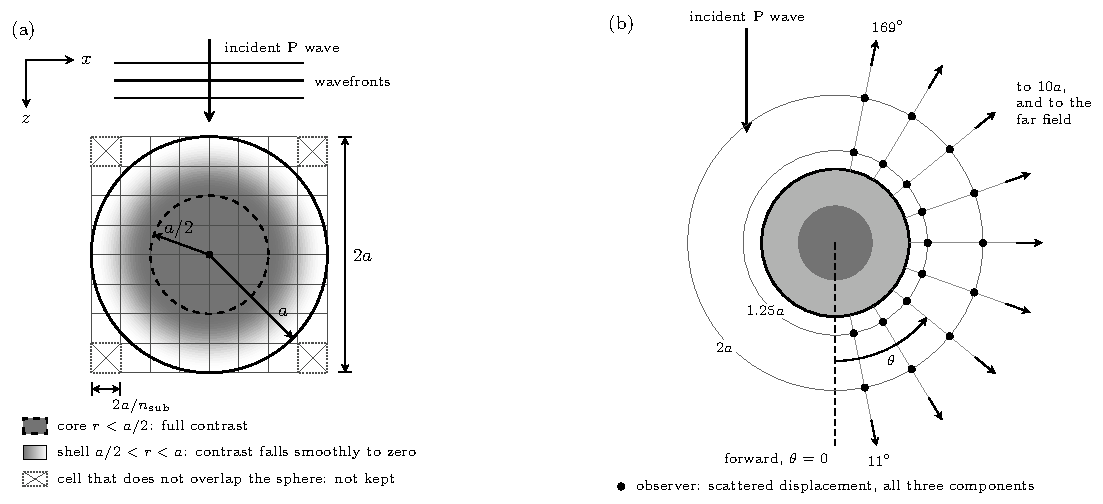
\includegraphics[width=\linewidth]{figures/fig_sphere.pdf}
\caption{The sphere experiment, in the section through the centre that contains the direction of
incidence. (a) The body and the grid. The contrast is full in the core $r<a/2$ and falls smoothly to zero
across the shell $a/2<r<a$. The circumscribing cube of side $2a$ is cut into $n_{\mathrm{sub}}^3$ cells,
here $n_{\mathrm{sub}}=8$; every cell that overlaps the sphere is kept and carries the projection of the
contrast it contains. A P plane wave is incident along $+z$. (b) The observers. The scattered
displacement is taken at nine scattering angles $\theta$, measured from the forward direction and equally
spaced from $11^\circ$ to $169^\circ$, on spheres of several radii about the centre, and compared with the
exact displacement at the same points.}
\label{fig:sphere}
\par\smallskip{\footnotesize\textit{Alt text:} Two panels. On the left, a disc on a square grid of
eight by eight cells: the inner half of the disc is uniformly dark, and the outer half fades from dark to
white at the rim, which is drawn as a solid circle; the four corner cells of the grid, which the disc does
not reach, are crossed out. Horizontal lines above the grid with a downward arrow mark the incident wave.
On the right, the same disc drawn smaller, with two concentric circles around it at one and a quarter and
at two radii; nine dots on each circle lie on nine rays from the disc, fanning from just off the downward,
forward direction to just off the upward, backward one, and each ray ends in an outward arrow.\par}
\end{figure}

\paragraph{A sphere without a staircase.} A voxelised sphere with a sharp surface changes its shape
with every grid. A sphere whose contrast falls smoothly to zero at its surface does not: the voxels
that cross the surface carry a vanishing contrast. The body here has a homogeneous core $r<a/2$
carrying the contrast of \S\ref{sec:convergence}, and across the shell $a/2<r<a$ the contrast falls to
zero as the smoothstep $s(x)=10x^3-15x^4+6x^5$, $x=(a-r)/(a-a/2)$, which vanishes like $(a-r)^3$ at the
surface. Its exact scattering follows, order by order, from the radial equations of
\citet{TakeuchiSaito1972}, integrated across the shell from the core's regular solutions and matched to
outgoing waves at $r=a$. The equations are derived symbolically from the equations of motion, and the
solution is checked against a sphere of homogeneous concentric shells in closed form, by unitarity and
reciprocity, and by an independent implementation that agrees to $2\times10^{-11}$
(\nb{TakeuchiSaito.wl}, \nb{ContinuumLimit\_GradedSphere.wl}, \path{scripts/crosscheck_graded_sphere.py}).
Each voxel carries the mean of the contrast over its cell. Table~\ref{tab:spheregraded} shows the
error falling at second order from $n_{\mathrm{sub}}=6$ to $24$ at both frequencies
(\path{scripts/pilot_graded_voxel_sphere.py}): the apparent order between successive grids is $2.02$
to $2.06$ at $k_Sa=0.5$ and $2.00$ at $k_Sa=1$, and the least-squares orders of
Fig.~\ref{fig:convergence}(d) are $2.045\pm0.004$ and $1.994\pm0.004$. With $24$ voxels across the
error is $1.8\times10^{-4}$ and $8.3\times10^{-4}$. At $n_{\mathrm{sub}}=4$ a voxel is as wide as
the graded shell and the order is not yet asymptotic. This is the order the layer predicts for the
mean-only voxel, and the first test of that prediction on a body with genuine three-dimensional
structure.

What makes the sequence this clean is that the voxel carries a single error. The collocation voxel
of the sharp sphere applied to this body, each cell at the profile's value at its centre and only the
cells whose centres lie inside the sphere kept, carries two: its own internal-field error and the
error of sampling the profile, both $O(h^2)$. Its error falls from $1.0\times10^{-1}$ at
$n_{\mathrm{sub}}=4$ to $4.7\times10^{-3}$, $2.6\times10^{-3}$, $6.4\times10^{-4}$ and
$2.3\times10^{-4}$ at $6$, $8$, $12$ and $16$, apparent orders $7.6$, $2.0$, $3.5$ and $3.6$ at
$k_Sa=0.5$, and at $k_Sa=1$ the apparent orders are $1.7$, $2.5$ and $2.4$ from $6$ to $16$: on
these grids its error is below the mean-only voxel's, but its apparent order is not that of any
single term and cannot be read from them. The same collocation voxel with the cell mean of the
contrast, and every overlapping cell kept, gives $3.4\times10^{-3}$, $1.9\times10^{-3}$ and
$8.2\times10^{-4}$ at $6$, $8$ and $12$, apparent orders $2.03$ and $2.05$: the sampling of the
profile was the second term, and with it removed the collocation and mean-only voxels differ only by
their constants, as in Table~\ref{tab:ratio}. The cell mean, with every
overlapping cell kept, represents the same body on every grid, and the order the layer predicts is
then the one observed.

The first-moment voxel of \S\ref{sec:fourth}, extended to three dimensions with a contrast linear in
each cell, converges at fourth order on this same sphere (Appendix~\ref{app:solver}): its apparent orders
are $4.01$ and $4.13$ where the discretisation error is isolated at weak contrast, and at the full
contrast its error with $16$ voxels across is $4.9\times10^{-6}$ and $5.9\times10^{-6}$, $82$ and
$317$ times below the mean-only voxel's on the same grid.

\paragraph{The near field, an impedance march, and a sharp sphere.} Three further tests are in
Appendix~\ref{app:sphere}. Read at finite distance, down to a quarter of a radius from the surface, the
graded sphere converges at the orders of the far field, second for the mean-only voxel and $3.8$ to
$3.95$ for the first-moment voxel, while the asymptotic readout would be in error there by $48\%$ to
$85\%$ (Table~\ref{tab:spherenear}). Against the impedance march of \citet{Haines2004}, which needs
far fewer unknowns, the first-moment voxel reaches the march's accuracy with six voxels across and
continues at close to fourth order below it, where the march is limited by the scattering between
the spheres of the periodic array it must solve (Table~\ref{tab:march}). And a sphere with a sharp
surface does not converge: its error tracks the volume of its staircase, which changes with the grid
(Table~\ref{tab:sphereraw}); the smooth sphere, like the layer, measures the scheme.

\FloatBarrier

\section{The error in two terms}\label{sec:twoterm}

Write the scattered far field as a series in the contrast: $u=T_1+T_2+\dots$, with $T_1$ the term of
first order (the Born term) and the rest the nonlinear part of the response. The error of the scheme
separates the same way.

\subsection{The first-order error needs no solve}\label{sec:born}

At first order in the contrast Eq.~\eqref{eq:system} is $M_\ell\psi_\ell=\langle Q,\psi^0\rangle_\ell$:
each cell holds the $L^2$ projection of the incident wave onto its field functions. The scheme's Born
term is therefore known from one pass over the cells, with no system to solve, and its difference from
the Born term of a finer representation (each cell's eight children with degree-two cells) is the
first-order error of the grid, cell by cell. On a grid of cells of two sizes this projected Born term
equals the weak-contrast limit of the full solver to $10^{-5}$ of its size.

\subsection{The wave factor of a cell}\label{sec:factor}

For a cell whose contrast is uniform the first-order error is a closed form. The cell represents the
incident wave $\mathrm{e}^{\mathrm{i}\bk_{\mathrm{in}}\cdot\bx}$ by its projection, and it radiates
towards the observer through the moments of $\mathrm{e}^{-\mathrm{i}\bk_{\mathrm{out}}\cdot\bx}$, with
$\bk_{\mathrm{out}}$ the P or the S wavevector in the direction of observation. Since
$\int_{-1}^{1}P_n(t)\,\mathrm{e}^{\mathrm{i}qt}\,\dd t=2\,\mathrm{i}^n j_n(q)$, with $j_n$ the spherical
Bessel function, the cell's Born far field is its exact Born far field times
\begin{equation}\label{eq:factor}
  1+E_p=\frac{\displaystyle\sum_{|a|\le p}\ \prod_{i=1}^{3}(2a_i+1)\,
        j_{a_i}\bigl(k_{\mathrm{in},i}h\bigr)\,j_{a_i}\bigl(k_{\mathrm{out},i}h\bigr)}
       {\displaystyle\prod_{i=1}^{3}j_0\bigl((k_{\mathrm{in},i}-k_{\mathrm{out},i})h\bigr)} .
\end{equation}
The sum over all degrees is the denominator (the addition theorem), so $E_p\to0$ as $p$ grows. Its
leading term is
\begin{equation}\label{eq:lead}
  E_p=-h^{2p+2}\sum_{|a|=p+1}\ \prod_{i=1}^{3}
      \frac{(2a_i+1)\,\bigl(k_{\mathrm{in},i}k_{\mathrm{out},i}\bigr)^{a_i}}{\bigl[(2a_i+1)!!\bigr]^2}
      +O\bigl(h^{2p+4}\bigr),
  \qquad E_0=-\frac{(\bk_{\mathrm{in}}\cdot\bk_{\mathrm{out}})\,d^2}{12}+\dots
\end{equation}
For a constant field the error of a cell therefore depends on the angle of scattering, vanishes at
right angles to the incident wave, and differs between the P and the S far field. Along one axis, with
$\bk_{\mathrm{out}}=\pm\bk_{\mathrm{in}}$ of magnitude $k$, Eq.~\eqref{eq:lead} is
$-(\pm1)^{p+1}c_p(kd)^{2p+2}$ with $c_p=(2p+3)/\bigl(4^{p+1}[(2p+3)!!]^2\bigr)$: the constants
$c_0=1/12$, $c_1=1/720$ and $c_2=1/100800$ of the layer, Eq.~\eqref{eq:cp}. The layer's
closed-form error is the one-dimensional case of the cell's.

\paragraph{Checks.} Equation~\eqref{eq:factor} is derived symbolically, built a second way without
Bessel functions (project, multiply, integrate over the cube) and found identical for $p=0$, $1$, $2$;
Eq.~\eqref{eq:lead} and its one-dimensional reduction are verified symbolically; and the implementation
used below agrees with $30$-digit values of the factor to $10^{-13}$ in $36$ cases. Against the solver,
on a homogeneous cube (which every grid of cubes represents exactly) at $k_SA=1$ for half-side $A$: the
Born far field divided by $1+E_p$ agrees across $p=0,1,2$ and two grids to $9\times10^{-7}$, where the
uncorrected fields differ by up to $14\%$; and the Born far field of $15$ cells of mixed sizes and
degrees equals the sum over the cells of exact contribution times factor to $2\times10^{-9}$.

\subsection{The rest is the projection error of the medium}\label{sec:rest}

Let $\cE_r$ be the relative projection error of the medium on the grid,
\begin{equation}\label{eq:proj}
  \cE_r=\frac{\sum_\ell\int_\ell\bigl(f-\Pi_rf\bigr)^2\,\dd V}{\int f^2\,\dd V},
\end{equation}
with $f(\bx)$ the profile of the contrast and $\Pi_r$ the $L^2$ projection onto the polynomials of
degree at most $r$ on each cell. Subtract from the error of the far field the first-order error of
\S\ref{sec:born}. What is left, divided by $\cE_r$, is one constant (Table~\ref{tab:twoterm}). The test
body is a sphere of radius $a$ with a uniform core of radius $0.75a$ and a shell across which the
contrast falls smoothly to zero, at $k_Sa=0.5$, whose exact solution is known; the error is the largest
difference of the far field from the exact one over nine scattering angles, relative to its peak.
\begin{table}[htbp]
\centering
\caption{The error of the far field in two terms, on the sphere with a graded shell. The rest is the
error less the first-order error, which is computed without a solve. $\cE$ is the relative projection
error of Eq.~\eqref{eq:proj} at the degree of the cells. The nonlinear fraction of the exact response
is $0.0151$.}\label{tab:twoterm}
\small
\begin{tabular}{@{}lrccc@{}}
\toprule
cells & number & error & error / $\cE$ & rest / $\cE$ \\
\midrule
constant ($p=r=0$) & $64$   & $8.17\times10^{-3}$ & $0.0309$ & $0.0149$ \\
 & $184$  & $3.18\times10^{-3}$ & $0.0235$ & $0.0151$ \\
 & $408$  & $1.61\times10^{-3}$ & $0.0196$ & $0.0154$ \\
 & $1256$ & $6.77\times10^{-4}$ & $0.0166$ & $0.0158$ \\
\midrule
degree one ($p=r=1$) & $64$  & $8.99\times10^{-4}$ & $0.0147$ & $0.0148$ \\
 & $184$ & $4.62\times10^{-4}$ & $0.0146$ & $0.0146$ \\
 & $408$ & $2.20\times10^{-4}$ & $0.0146$ & $0.0146$ \\
\bottomrule
\end{tabular}
\end{table}
For constant cells the ratio of error to projection error varies by a factor of $1.86$ across the
grids; the rest over the projection error varies by $1.06$. For degree-one cells the first-order error is small and both ratios are near $0.0146$. The constant
is close to the nonlinear fraction of the exact response, $\nu=\lvert u-T_1\rvert/\lvert u\rvert=0.0151$.
This is the law of the layer (\S\ref{sec:hetero}) carried to three dimensions: the error of the
nonlinear part is that part times the relative projection error of the medium, times a factor of order
one that \S\ref{sec:factor3d} derives. It holds for constant cells as it does for degree-one cells, once the
first-order error is accounted for; without that, constant cells appear not to follow it.

\subsection{The factor of the second term in three dimensions}\label{sec:factor3d}

\paragraph{Why a factor appears.} In the layer the relative error of the term of second order in the
contrast, $T_2$, equals the relative projection error exactly in the long-wave limit, because there the
kernel that maps a strain source to the strain it scatters is local: the once-scattered strain is the
profile itself, and a cell holds it as the profile's projection (\S\ref{sec:hetero}). In three
dimensions the same kernel has, besides its local part, a part that falls as the inverse cube of the
distance. The once-scattered strain then depends on how the residual of the projection is arranged in
space, and cubic cells arrange it along their axes. The question is what replaces the
layer's equality.

\paragraph{The second-order term of the scheme.} Take a stiffness contrast $f(\bx)\,\Delta\mathbf{C}$,
with $f$ the profile, struck by a uniform strain $\boldsymbol\varepsilon_{\mathrm{in}}$ and observed
through a uniform strain $\boldsymbol\varepsilon_{\mathrm{out}}$ of the outgoing P or S wave (the
long-wave limit, in which the derivation is made; the test below is at $k_Sa=0.125$). The second
term is the quadratic form $T_2=\langle f,Kf\rangle$ of the operator $K$ whose Fourier multiplier is
\begin{equation}\label{eq:mfactor}
  m(\hat{\boldsymbol\xi})=\mathbf{a}:\boldsymbol\Gamma(\hat{\boldsymbol\xi}):\mathbf{b},\qquad
  \mathbf{a}=\Delta\mathbf{C}:\boldsymbol\varepsilon_{\mathrm{out}},\quad
  \mathbf{b}=\Delta\mathbf{C}:\boldsymbol\varepsilon_{\mathrm{in}},
\end{equation}
with $\boldsymbol\Gamma$ the static strain Green operator of the background, which depends only on the
direction $\hat{\boldsymbol\xi}$ of the wavevector:
$m=\hat{\boldsymbol\xi}\cdot\tfrac12(\mathbf{a}\mathbf{b}+\mathbf{b}\mathbf{a})\cdot\hat{\boldsymbol\xi}/\mu
-\tfrac{\lambda+\mu}{\mu(\lambda+2\mu)}(\hat{\boldsymbol\xi}\cdot\mathbf{a}\cdot\hat{\boldsymbol\xi})
(\hat{\boldsymbol\xi}\cdot\mathbf{b}\cdot\hat{\boldsymbol\xi})$. Cells whose field and contrast are
of the same degree compute $\langle\Pi f,K\Pi f\rangle$, $\Pi$ the projection of \S\ref{sec:rest}, so
with $g=f-\Pi f$ the residual,
\begin{equation}\label{eq:t2factor}
  \frac{T_2-T_2^{\mathrm{scheme}}}{T_2}=\cE\,F,\qquad
  F=\frac{2\langle g,Kf\rangle-\langle g,Kg\rangle}{\langle f,Kf\rangle\,\cE}.
\end{equation}
In the layer $F=1$. For a body whose spectrum is the same in every direction, as a radial profile's is,
$\langle f,Kf\rangle=\bar m\lVert f\rVert^2$ with
$\bar m=\operatorname{tr}\bigl(\tfrac12(\mathbf{a}\mathbf{b}+\mathbf{b}\mathbf{a})\bigr)/(3\mu)
-\tfrac{\lambda+\mu}{\mu(\lambda+2\mu)}\bigl(\operatorname{tr}\mathbf{a}\operatorname{tr}\mathbf{b}
+2\,\mathbf{a}:\mathbf{b}\bigr)/15$, the average of $m$ over directions. The two remaining forms are
evaluated as the cells shrink, from what the residual looks like inside one cell.

\paragraph{Constant cells.} In a cell of half-width $h$ the residual is $\nabla f\cdot(\bx-\bx_\ell)$, a
sum of three sawtooths, one along each axis. Two facts settle the two forms. Its first moments and its
energy carry the same constant, $h^2/3$, and its second moments vanish, so its transform at small
wavenumbers is $(h^2/3)\lvert\boldsymbol\xi\rvert^2\hat f$, the same in every direction, and
$2\langle g,Kf\rangle\to2\bar m\lVert g\rVert^2$. And a sawtooth has no mean and its harmonics lie
on its own axis, carrying all its energy, so $\langle g,Kg\rangle\to m_{\mathrm{ax}}\lVert
g\rVert^2$, with $m_{\mathrm{ax}}$ the mean of $m$ over the three cube axes. Hence
\begin{equation}\label{eq:F0}
  F_0=2-\frac{m_{\mathrm{ax}}}{\bar m}.
\end{equation}
The cell enters through its axes: a residual arranged along them sees the operator along them, while the
body sees it averaged over all directions.

\paragraph{Degree-one cells.} The residual is the quadratic part of $f$ less its projection,
$\tfrac12\sum_iH_{ii}(x_i^2-h^2/3)+\sum_{i<j}H_{ij}x_ix_j$ with $H$ the second derivatives of $f$.
Its energy is $\sum_iH_{ii}^2h^4/45+\sum_{i<j}H_{ij}^2h^4/9$ per unit volume, and its second moments,
$2h^4/45$ on the diagonal and $h^4/9$ off it, give its transform at small wavenumbers as
$h^4W(\boldsymbol\xi)\hat f$ with
$W=\sum_k\xi_k^4/45+\sum_{k<l}\xi_k^2\xi_l^2/9$, which is no longer the same in every direction. The
parabolas $x_i^2-h^2/3$ have their spectrum on their axes; each product $x_ix_j$ of two sawtooths has its
spectrum on the lattice of the $(i,j)$ plane, at the points $(m,n)$, $m,n\neq0$, with weights
$1/(m^2n^2)$, over which the averages of $u^2v^2$ and $u^4$ ($u$, $v$ the direction cosines) are
$6G/\pi^2-\tfrac25$ and $\tfrac9{10}-6G/\pi^2$, $G$ being Catalan's constant, from the lattice sum
$\sum_{m,n\neq0}(m^2+n^2)^{-2}=4\zeta(2)\beta(2)-4\zeta(4)$. For a radial profile
\begin{equation}\label{eq:F1}
  F_1=\frac{2\langle Wm\rangle-\tfrac1{225}\sum_im(\mathbf{e}_i)-\tfrac1{135}\sum_{i<j}M_{ij}}
            {\tfrac{8}{225}\,\bar m},
\end{equation}
with $\langle Wm\rangle$ the average of $Wm$ over directions and $M_{ij}$ the average of $m$ over the
lattice of the $(i,j)$ plane. A constant $m$ gives $F_0=F_1=1$, and so does a layer.

\paragraph{Closed forms.} For an incident P wave and an outgoing SV wave the factors depend on the
background alone, not on the contrast or the angle:
\begin{equation}\label{eq:Fps}
  F_0^{\mathrm{PS}}=\frac{6\lambda+11\mu}{3\lambda+8\mu},\qquad
  F_1^{\mathrm{PS}}=\frac{5\bigl[(57\lambda+85\mu)\pi^2-315G(\lambda+\mu)\bigr]}{28\pi^2(3\lambda+8\mu)},
\end{equation}
$1.516$ and $1.337$ for the background of the tests ($\alpha=5000$, $\beta=3000$\,m\,s$^{-1}$). For an
outgoing P wave the factors are ratios of expressions linear in $\cos2\theta$, $\theta$ the scattering
angle; for the contrast of the tests $F_0^{\mathrm{PP}}$ runs from $1.101$ near forward and back
scattering to $0.923$ at right angles, and $F_1^{\mathrm{PP}}$ from $1.066$ to $0.950$.

\paragraph{The test.} The derivation is symbolic, in $31$ checks, from the Navier equation to the closed
forms (\path{Mathematica/AdaptiveOctree_T2Factor.wl}). It is tested two ways on a sphere of radius
$a=10$\,m whose contrast is uniform within $a/2$ and falls smoothly to zero at the surface, with a
stiffness contrast, at $k_Sa=0.125$: by the scheme itself,
whose $T_2$ is set against the exact one, angle by angle and wave by wave
(\path{scripts/measure_t2_law_3d.py}); and by evaluating the two forms of Eq.~\eqref{eq:t2factor}
directly, by fast Fourier transform on a grid finer than the cells (\path{scripts/measure_t2_quadratic_forms.py}); the details are in Appendix~\ref{app:experiments}.
\begin{table}[htbp]
\centering
\caption{The factor $F$ of Eq.~\eqref{eq:t2factor}: the scheme on $8$ cells across, the direct
evaluation on finer grids ($32$ cells for constant, $24$ for degree one), and the limit,
Eqs.~\eqref{eq:F0}--\eqref{eq:Fps}.}\label{tab:t2factor}
\small
\begin{tabular}{@{}lcccccc@{}}
\toprule
 & \multicolumn{3}{c}{constant cells} & \multicolumn{3}{c}{degree-one cells} \\
outgoing wave & scheme & direct & limit & scheme & direct & limit \\
\midrule
P at $0.2$\,rad & $1.074$ & $1.092$ & $1.101$ & $1.073$ & $1.067$ & $1.066$ \\
P at $\pi/2$    & $0.944$ & $0.930$ & $0.923$ & $0.948$ & $0.949$ & $0.950$ \\
SV at $0.2$\,rad & $1.376$ & $1.470$ & $1.516$ & $1.356$ & $1.342$ & $1.337$ \\
\bottomrule
\end{tabular}
\end{table}
On $8$ cells the scheme and the direct evaluation agree to $1\%$ where both are computed on the same
grid, which confirms Eq.~\eqref{eq:t2factor}. As the cells shrink both approach the limit: for constant
cells $\langle g,Kg\rangle/(\bar m\lVert g\rVert^2)$ goes $0.926$, $0.909$, $0.902$ on $8$, $16$ and
$32$ cells against its limit $m_{\mathrm{ax}}/\bar m=0.899$ (outgoing P at $0.2$\,rad), slowly, the
distance falling as about $h^{1.7}$; for degree-one cells the factor is within $0.4\%$ of the limit by $24$
cells. The scheme on $8$ cells is three quarters of the way to the limit
for constant cells.

\paragraph{What it means for the second term.} The second term of the error is the nonlinear part of the
response times the relative projection error times $F$, a factor of order one that depends on the
background, the direction of scattering and the type of wave, and on the cells through their axes, not
on the grid. For this background and contrast it lies between $0.92$ and $1.52$ for constant cells and
between $0.95$ and $1.34$ for degree-one cells, and it is one in a layer, which is why the layer's law is an
equality. The constant of Table~\ref{tab:twoterm}, formed from the largest error over the angles and
with every order above the first included, is $0.96$ to $1.05$ times $\nu$, inside that range. The second term is therefore known before
the solve to within $F$, and in closed form once the direction of observation is chosen. The derivation
holds for the term of second order, in the long-wave limit, for a body whose spectrum is isotropic; the
terms of higher order are measured, not derived.

\subsection{The nonlinear fraction without a solve}\label{sec:nu}

\paragraph{Why it is needed.} The second term of the error is $\nu\,\cE\,F$, and of its three factors
only the nonlinear fraction $\nu=\max\lvert u-T_1\rvert/\max\lvert u\rvert$ (the maxima over the angles
of observation) would need a solve: one solve on a coarse grid that resolves the medium, taking
$\lvert u-T_1\rvert/\lvert u\rvert$ of that grid. That estimate is low, by up to a quarter for constant
cells (Table~\ref{tab:nu}), and the reason is the second term itself: the coarse grid's nonlinear part is
low by its own relative projection error.

\paragraph{The method.} The scheme's response is a series in the contrast, $\psi=\sum_n\psi_n$ with
$M\psi_1=b$ and $M\psi_{n+1}=KE\,\psi_n$, $M$ the Gram matrices of the cells, $b$ the moments of the
incident wave and $KE$ the coupling times the contrast (Eq.~\eqref{eq:system}). The first term is the
Born term of \S\ref{sec:born}; each further term costs one product with the assembled matrix and no
solve. Two facts make a few terms enough. On the exact solutions the terms of second and third order
carry the nonlinear fraction to $0.2\%$ (on the three bodies of Table~\ref{tab:nu}; $T_2$ alone to
$4\%$), because $\lvert T_3\rvert/\lvert T_2\rvert$ is $0.03$ to $0.04$. And on the coarse grid the
nonlinear part of the scheme is low by its relative projection error $\cE$, which is known before the
solve (\S\ref{sec:rest}). The estimate is therefore
\begin{equation}\label{eq:nuest}
  \nu\approx\frac{\max\lvert T_2+T_3\rvert/(1-\cE)}{\max\bigl\lvert T_1+(T_2+T_3)/(1-\cE)\bigr\rvert},
\end{equation}
with $T_n$ the far fields of the scheme's terms on the coarse grid and the factor $F$ of
\S\ref{sec:factor3d} taken as one.

\paragraph{The result.} Table~\ref{tab:nu} sets the estimates against the exact nonlinear fraction on
three bodies, for constant and degree-one cells. The coarse grid resolves the medium: it is refined
where a cell's share of the projection error exceeds $10^{-2}$, starting from eight cells
(\path{scripts/measure_octree_nu_estimate.py}; Appendix~\ref{app:experiments}).
\begin{table}[htbp]
\centering
\caption{The nonlinear fraction estimated on a coarse grid, over its exact value. ``Solve'' is the
earlier estimate (one dense solve); Eq.~\eqref{eq:nuest} uses two products with the matrix and the
grid's projection error $\cE$.}\label{tab:nu}
\small
\begin{tabular}{@{}llrccccc@{}}
\toprule
body & cells & number & $\cE$ & exact $\nu$ & solve & $T_2/(1-\cE)$ & Eq.~\eqref{eq:nuest} \\
\midrule
thin shell, $k_Sa=0.5$ & constant & $64$ & $0.264$ & $0.0151$ & $0.746$ & $1.047$ & $1.014$ \\
 & degree one & $64$ & $0.061$ & & $0.940$ & $1.039$ & $1.000$ \\
feature $0.2a$--$0.5a$, $k_Sa=1$ & constant & $120$ & $0.175$ & $0.0107$ & $0.816$ & $1.017$ & $0.990$ \\
 & degree one & $120$ & $0.036$ & & $0.963$ & $1.028$ & $0.999$ \\
feature $0.1a$--$0.3a$, $k_Sa=1$ & constant & $176$ & $0.145$ & $0.0059$ & $0.854$ & $1.025$ & $1.000$ \\
 & degree one & $176$ & $0.015$ & & $0.985$ & $1.027$ & $0.999$ \\
\bottomrule
\end{tabular}
\end{table}
The estimate of Eq.~\eqref{eq:nuest} is within $1.4\%$ of the exact value in all six cases; the solve
is $25\%$ low at worst, and the second-order term alone, corrected, is $2\%$ to $5\%$ high, which is
the share of the third-order term.

\paragraph{What it means.} Both terms of the error are now known before the solve, without any solve:
the first from one pass over the cells, the second from the relative projection error, the factor
$F$ in closed form, and the nonlinear fraction from two products with the matrix of a coarse grid. The
estimate rests on the law of \S\ref{sec:rest} applied to the coarse grid, and has been tested on three
bodies at two frequencies.

\subsection{The terms of third and higher order}\label{sec:higher}

\paragraph{Why they matter.} The law of \S\ref{sec:rest} was measured on the whole nonlinear part,
$u-T_1$, and \S\ref{sec:factor3d} derived the factor of its second-order term only. Each further term
carries an error of its own, and in the layer the whole nonlinear part does not follow the
second-order law: all orders together give $0.90$ to $0.94$ times $\cE$ where $T_2$ alone gives one
(Appendix~\ref{app:borndefect}).

\paragraph{The layer, exactly.} In the long-wave limit the layer's kernel is local, the strain scattered
by a stiffness contrast being $c\,f\boldsymbol\varepsilon$ with $c=-\Delta M/M_P$, $M_P=\lambda+2\mu$. With
field and contrast of the same degree in each cell the scheme's term of order $n$ is then
$c^{\,n-1}\!\int(\Pi f)^n\,\dd z$ against the exact $c^{\,n-1}\!\int f^n\,\dd z$, for $n\le3$ at every degree and for
every $n$ in constant cells, so the relative error of each term is a property of the profile,
\begin{equation}\label{eq:en}
  e_n=\frac{\int f^n\,\dd z-\int(\Pi f)^n\,\dd z}{\int f^n\,\dd z},\qquad e_2=\cE .
\end{equation}
Summed, the exact strain is $\boldsymbol\varepsilon_0/(1-cf)$, and the scheme's is the Galerkin solution
of $\boldsymbol\varepsilon=\boldsymbol\varepsilon_0+c\,f\boldsymbol\varepsilon$ in each cell separately,
on that cell's polynomials: the error of the whole nonlinear part is the single site's, in closed form.
On the heterogeneous layer of \S\ref{sec:hetero} (profile $1+\tfrac12\sin(2\pi z/D)$) at
$\omega=30$\,rad\,s$^{-1}$ the scheme's $T_3$ has the error $e_3$ of Eq.~\eqref{eq:en} to $10^{-4}$, for
constant, degree-one and degree-two cells on $4$ to $16$ cells, in reflection and in transmission, and to
$0.5\%$ at $\omega=300$\,rad\,s$^{-1}$; $e_3/\cE=2.455$ on every grid, which is
$3\,\langle f\rangle_{g^2}\int f^2\,\dd z/\int f^3\,\dd z$ with $\langle f\rangle_{g^2}$ the mean of the profile weighted
by the squared residual. Because $T_3/T_2=-0.078$, the second and third terms together have $0.877$ times
$\cE$, and the whole nonlinear part at the full contrast $0.896$ times $\cE$, which the cell-by-cell
Galerkin solution reproduces to four digits with $c=-0.0640$ from the contrast; the exact layer's
$T_3/T_2$ returns the same $c$ to five digits (\path{scripts/measure_layer_t3_law.py}). This is the
$0.90$ of Appendix~\ref{app:borndefect}.

\paragraph{Three dimensions.} The kernel is not local, and the third-order term involves the
once-scattered strain fields themselves: with $\mathbf{u}_{\mathbf{b}}=\boldsymbol\Gamma*(f\mathbf{b})$ and
$\mathbf{u}_{\mathbf{a}}=\boldsymbol\Gamma*(f\mathbf{a})$ in the notation of Eq.~\eqref{eq:mfactor},
$T_3=\int f\,\mathbf{u}_{\mathbf{a}}:\Delta\mathbf{C}:\mathbf{u}_{\mathbf{b}}\,\dd V$, and constant cells compute
$\int\Pi f\,\Pi\mathbf{U}_{\mathbf{a}}:\Delta\mathbf{C}:\Pi\mathbf{U}_{\mathbf{b}}\,\dd V$ with
$\mathbf{U}=\boldsymbol\Gamma*(\Pi f\,\cdot)$. Its factor $F_3$, defined as $F$ is by
Eq.~\eqref{eq:t2factor}, therefore depends on the body's own field and not only on averages of $m$.

\paragraph{The closed form.} The difference is expanded to second order in the half-width, as for
the second term, with $\mathbf{u}=\Pi\mathbf{u}+\mathbf{u}'$ the cell decomposition of each field. Four
pieces appear, each from a lemma already in hand. The residual $g$ meets a smooth field
$w_{\mathbf{ab}}=\mathbf{a}:\boldsymbol\Gamma*(f\,\Delta\mathbf{C}:\mathbf{u}_{\mathbf{b}})$ through its first
moments, giving $(h^2/3)\nabla f\cdot\nabla w_{\mathbf{ab}}$. The field scattered by the residual is a
sawtooth on each cube axis carrying $\boldsymbol\Gamma$ on that axis,
$\mathbf{G}_{i\mathbf{b}}=\boldsymbol\Gamma(\mathbf{e}_i)\mathbf{b}$, with amplitude $\partial_if$. The
smooth fields vary across a cell as sawtooths of amplitude $\partial_i\mathbf{u}$. And a cell's mean of
a product of three fields splits exactly into the product of the means and the means of products of
the departures. The terms in $(\partial_if)^2\mathbf{G}\mathbf{G}$ cancel, and
\begin{equation}\label{eq:F3}
\begin{split}
  \frac{T_3-T_3^{\mathrm{scheme}}}{h^2/3}=\int\Bigl[&\nabla f\cdot\nabla(w_{\mathbf{ab}}+w_{\mathbf{ba}})\\
  &+f\sum_i\bigl(\partial_i\mathbf{u}_{\mathbf{a}}:\Delta\mathbf{C}:\partial_i\mathbf{u}_{\mathbf{b}}
     -\partial_if\,(\partial_i\mathbf{u}_{\mathbf{a}}:\Delta\mathbf{C}:\mathbf{G}_{i\mathbf{b}}
     +\mathbf{G}_{i\mathbf{a}}:\Delta\mathbf{C}:\partial_i\mathbf{u}_{\mathbf{b}})\bigr)\\
  &+\sum_i\partial_if\,\bigl(\mathbf{u}_{\mathbf{a}}:\Delta\mathbf{C}:\partial_i\mathbf{u}_{\mathbf{b}}
     +\partial_i\mathbf{u}_{\mathbf{a}}:\Delta\mathbf{C}:\mathbf{u}_{\mathbf{b}}\bigr)\\
  &-\sum_i(\partial_if)^2\bigl(\mathbf{u}_{\mathbf{a}}:\Delta\mathbf{C}:\mathbf{G}_{i\mathbf{b}}
     +\mathbf{G}_{i\mathbf{a}}:\Delta\mathbf{C}:\mathbf{u}_{\mathbf{b}}\bigr)\Bigr]\,\dd V,
\end{split}
\end{equation}
with $F_3=(T_3-T_3^{\mathrm{scheme}})/(T_3\cE)$ and $\cE=(h^2/3)\int\lvert\nabla f\rvert^2\dd V/\int
f^2\dd V$. It is a closed form in the sense of Eq.~\eqref{eq:F0}: the cells enter only through
$\boldsymbol\Gamma$ on their three axes, and everything else is an integral of the body's smooth,
once-scattered static fields, so it needs no grid of cells. In a layer every field is local and the
integrand is $3ff'^2\,\mathbf{G}_{\mathbf{a}}:\Delta\mathbf{C}:\mathbf{G}_{\mathbf{b}}$, which is the
layer's $e_3$; the same expansion of the second term gives Eq.~\eqref{eq:F0}. The algebra is verified
symbolically in $7$ checks (\path{Mathematica/AdaptiveOctree_F3.wl}).

\paragraph{The test.} Equation~\eqref{eq:F3} is evaluated on the sphere of \S\ref{sec:factor3d} by fast
Fourier transform of the smooth fields alone, converged in resolution and in the padding against the
images of the periodic box (\path{scripts/measure_f3_closed_form.py}; its value of $F$ for the second
term is $1.1016$ against the exact $1.1009$). It is set against two evaluations on cells: the scheme,
whose terms are those of its Born series (\path{scripts/measure_t3_law_3d.py}), and the cell forms
computed directly with $\boldsymbol\Gamma$ applied by fast Fourier transform
(\path{scripts/measure_t3_tensor_forms.py}). On $4$ cells across the last two agree to $0.3\%$ for the
outgoing P wave. The details of every measurement are in Appendix~\ref{app:experiments}.

\paragraph{Degree-one cells.} With the field and the contrast in $1,x_1,x_2,x_3$ the projection on the
outgoing side can be moved onto the profile, and the scheme's term is
$\int\Pi f\,\mathbf{U}_{\mathbf{a}}:\Delta\mathbf{C}:\Pi\mathbf{U}_{\mathbf{b}}\,\dd V$, with one
projection, on the incident side; for constant cells it is the form above. The residual is now the
quadratic part of the profile less its projection, $\tfrac12\sum_if_{,ii}P_i+\sum_{i<j}f_{,ij}Q_{ij}$ with
$P_i=x_i^2-h^2/3$ and $Q_{ij}=x_ix_j$ (local coordinates), and every term reduces to two cell rules. A
cell-scale function meets a smooth one through their second derivatives,
\begin{equation}\label{eq:Brule}
  B(S,T)=h^4\Bigl[\sum_i\frac{S_{,ii}T_{,ii}}{45}+\sum_{i<j}\frac{S_{,ij}T_{,ij}}{9}\Bigr],
\end{equation}
and the field the residual scatters carries $\boldsymbol\Gamma$ on the axes for its parabolas and
$\mathbf{M}_{ij}$, the average of $\boldsymbol\Gamma$ over the lattice of the $(i,j)$ plane with
$\langle u^2v^2\rangle=6G/\pi^2-\tfrac25$ (\S\ref{sec:factor3d}), for its products. The term in two
scattered residual fields is absent, because the projection removes the part of $\mathbf{U}_{\mathbf{b}}$
at the scale of the cell, and
\begin{equation}\label{eq:F3lin}
\begin{split}
  T_3-T_3^{\mathrm{scheme}}=\int\Bigl[&B(f\Delta\mathbf{C}\mathbf{u}_{\mathbf{a}},\mathbf{u}_{\mathbf{b}})
   +B(f,w_{\mathbf{ab}}+w_{\mathbf{ba}}+\mathbf{u}_{\mathbf{a}}:\Delta\mathbf{C}:\mathbf{u}_{\mathbf{b}})
   -H(f\Delta\mathbf{C}\mathbf{u}_{\mathbf{a}},f;\mathbf{b})\\
  &-f\,K(f;\mathbf{a},\mathbf{u}_{\mathbf{b}})-\mathbf{u}_{\mathbf{a}}:\Delta\mathbf{C}:B(f,\mathbf{u}_{\mathbf{b}})
   -K_2(f;\mathbf{a}):\Delta\mathbf{C}:\mathbf{u}_{\mathbf{b}}\Bigr]\dd V,
\end{split}
\end{equation}
where $H$, $K$ and $K_2$ are $B$ with one smooth factor replaced by the scattered residual,
\begin{align*}
  H(S,f;\mathbf{b})&=h^4\Bigl[\sum_i\frac{S_{,ii}:\mathbf{G}_{i\mathbf{b}}\,f_{,ii}}{45}
    +\sum_{i<j}\frac{S_{,ij}:\mathbf{M}_{ij}\mathbf{b}\,f_{,ij}}{9}\Bigr],\\
  K(f;\mathbf{a},\mathbf{u})&=h^4\Bigl[\sum_i\frac{f_{,ii}\,\mathbf{G}_{i\mathbf{a}}:\Delta\mathbf{C}:\mathbf{u}_{,ii}}{45}
    +\sum_{i<j}\frac{f_{,ij}\,\mathbf{M}_{ij}\mathbf{a}:\Delta\mathbf{C}:\mathbf{u}_{,ij}}{9}\Bigr],\\
  K_2(f;\mathbf{a})&=h^4\Bigl[\sum_i\frac{f_{,ii}^2\,\mathbf{G}_{i\mathbf{a}}}{45}
    +\sum_{i<j}\frac{f_{,ij}^2\,\mathbf{M}_{ij}\mathbf{a}}{9}\Bigr],
\end{align*}
and $\cE=h^4\int[\sum_if_{,ii}^2/45+\sum_{i<j}f_{,ij}^2/9]\dd V/\int f^2\dd V$. In a layer the integrand is
$(h^4/45)\,\kappa\,(6f'^2f''+3ff''^2)$, $\kappa=\mathbf{G}_{\mathbf{a}}:\Delta\mathbf{C}:\mathbf{G}_{\mathbf{b}}$,
which is the direct expansion of $\int f^3-\int(\Pi f)^3$; and the same rules give the second term as
$2B(f,\mathbf{a}:\mathbf{u}_{\mathbf{b}})-\mathbf{a}:K_2(f;\mathbf{b})$, whose ratio is the $F_1$ of
Eq.~\eqref{eq:F1}. The algebra is verified in $8$ checks (\path{Mathematica/AdaptiveOctree_F3Linear.wl}).
The closed form gives $F_3=1.475$, $1.428$ and $1.387$ for the outgoing P wave at $0.2$, $0.885$ and
$\pi/2$\,rad and $1.892$ for the SV wave, and its value of $F_1$ for the second term is $1.0672$ against
the exact $1.0659$. The direct evaluation on cells approaches it at second order in the cell size, and
extrapolated from $16$ and $24$ cells gives $1.475$, $1.436$, $1.404$ and $1.874$. The scheme on $8$
cells gives $1.350$, $1.299$, $1.254$ and $1.79$, which the direct evaluation on $8$ cells reproduces
($1.351$, $1.264$ and $1.79$): for degree-one cells $F_3$, unlike $F_1$, is still far from its limit on $8$
cells.

\begin{table}[htbp]
\centering
\caption{The factors of the second and third terms and of the whole nonlinear part, $k_Sa=0.125$: the
scheme on $8$ cells across, the direct evaluation of $F_3$ (constant cells: $32$ cells, outgoing P, the SV
wave not converged; degree-one cells: extrapolated from $16$ and $24$), and the closed forms,
Eqs.~\eqref{eq:F3} and \eqref{eq:F3lin}.}\label{tab:higher}
\small
\setlength{\tabcolsep}{4pt}
\begin{tabular}{@{}lcccccc@{}}
\toprule
outgoing wave & $F$ (scheme) & $F_3$ (scheme) & $F_3$ (direct) & $F_3$ (closed form) & $T_3/T_2$ & nonlinear part \\
\midrule
\multicolumn{7}{@{}l}{constant cells} \\
P at $0.2$\,rad & $1.073$ & $1.600$ & $1.586$ & $1.594$ & $-0.036$ & $1.054$ \\
P at $\pi/2$    & $0.944$ & $1.494$ & $1.417$ & $1.410$ & $-0.042$ & $0.921$ \\
SV at $0.2$\,rad & $1.375$ & $2.145$ & & $2.46$ & $-0.021$ & $1.358$ \\
\multicolumn{7}{@{}l}{degree-one cells} \\
P at $0.2$\,rad & $1.066$ & $1.350$ & $1.475$ & $1.475$ & $-0.036$ & $1.056$ \\
P at $\pi/2$    & $0.948$ & $1.254$ & $1.404$ & $1.387$ & $-0.042$ & $0.935$ \\
SV at $0.2$\,rad & $1.341$ & $1.79$ & $1.874$ & $1.892$ & $-0.021$ & $1.332$ \\
\bottomrule
\end{tabular}
\end{table}
The direct evaluation converges as the cells shrink ($1.62$, $1.58$, $1.59$ on $8$, $16$ and $32$
cells, outgoing P at $0.2$\,rad) to the closed form, $1.594$, and agrees with it to $0.5\%$ at both
angles. The scheme on $8$ cells is three quarters of the way to it for the SV wave, as it is for the
second term. The nonlinear part's factor is the mean of the terms' factors
weighted by the terms: $(F+F_3T_3/T_2)/(1+T_3/T_2)=1.054$ against the measured $1.054$, so the fourth
and higher terms contribute $0.05\%$.

\paragraph{What it means.} Every order has its own factor, larger than the second's, and the factor of the
nonlinear part is their mean weighted by the terms. Where the contrast is moderate the second term
dominates ($\lvert T_3/T_2\rvert$ is $0.02$ to $0.04$ here) and the nonlinear part's factor is $F$ to
within $\lvert T_3/T_2\rvert(F_3-F)$, two percent here; the estimate of \S\ref{sec:nu} already carries the
third term. In the layer the whole series is derived; in three dimensions the factor of the third
term is derived in closed form for constant and for degree-one cells, Eqs.~\eqref{eq:F3} and \eqref{eq:F3lin},
and those of the higher terms are measured.

\section{Matching the bases}\label{sec:which}

\paragraph{A smooth medium: the degrees must be matched.} The test body is a sphere of radius $a$ whose
contrast is a weak halo, falling smoothly from $5\%$ of the central value to zero across the whole radius,
plus a compact feature in which it falls from the central value to the halo between $0.1a$ and $0.3a$, at
$k_Sa=1$ (Appendix~\ref{app:experiments}). Hold the contrast constant in every cell and raise the field to
degree one. The error rises, at four times the unknowns: from $7.15\times10^{-3}$ to $8.31\times10^{-3}$ on
the uniform grid of $408$ cells. The two terms, computed without a solve, predict it
($1.11\times10^{-2}$ against $1.34\times10^{-2}$). On a smoothly varying medium the first-order error of a
cell with a constant contrast is not the wave's: it is the error of holding the contrast constant, which a
richer field cannot repair, and with a constant field the wave's error partly cancels it. This is the rule
of \S\ref{sec:hetero} that the two bases must be matched, now with the error predicted before the
solve.

\paragraph{A medium that is piecewise constant.} Where the medium is constant on each cell, a constant
contrast is exact, the second term vanishes, and the degree is better spent on the field. That needs cells
whose faces follow the interfaces of the medium; where an interface falls inside a cell, a richer field is
worse than a constant one, as on the smooth body, and for the scalar problem \citet{Anderson2026} likewise
find that high order is lost at jumps of the medium unless the grid follows them.


\section{Discussion}\label{sec:discussion}

Figure~\ref{fig:convergence} collects the convergence of every test, with the order fitted to each by
least squares (\path{scripts/plot_convergence_orders.py}).

\begin{figure}[t]
\centering
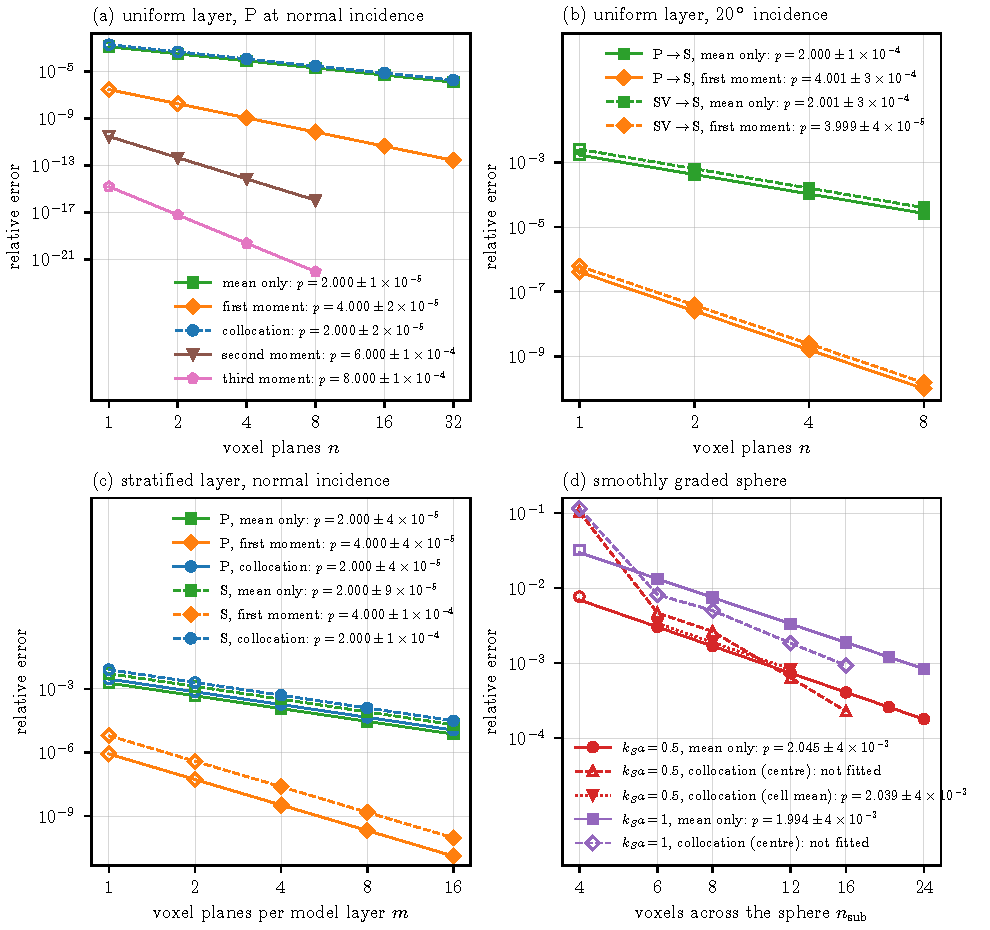
\includegraphics[width=\linewidth]{figures/fig_convergence.pdf}
\caption{Convergence of every test, with least-squares regression lines. Each line fits
$\log e=c-p\log n$ to the filled points; open points are pre-asymptotic and are not fitted. The legend
gives the order $p$ and its standard error. The marker, and in colour the hue, marks the scheme, so
that the figure reads in grey scale: collocation (circles; Eq.~\eqref{eq:collocation}),
the mean-only voxel (squares) and the voxels carrying Legendre moments to degree $p=1$ (diamonds), $2$
(triangles) and $3$ (pentagons) (Eqs.~\eqref{eq:galerkin} and \eqref{eq:bloch}). (a)~The uniform layer, P reflection at normal
incidence ($D=2$\,m, $\omega=300$\,rad\,s$^{-1}$, the contrast of \S\ref{sec:convergence}), fitted from
$n=4$; the collocation line is dashed and lies on the mean-only line, from which its constant differs
only by the factor $3/2$ of Table~\ref{tab:ratio}; the second- and third-moment voxels, computed in 40-digit arithmetic, fitted from $n=2$. (b)~The uniform layer at $20^\circ$, fitted from
$n=2$: the S wave converted from incident P (solid) and reflected from incident SV (dashed).
(c)~The stratified layer of \S\ref{sec:hetero}, reflection at normal incidence for P (solid) and S
(dashed), against the number $m$ of voxel planes per model layer, fitted from $m=4$. (d)~The
smoothly graded sphere of \S\ref{sec:sphere} against its exact solution, for $n_{\mathrm{sub}}$ voxels
across: the mean-only voxel, fitted from $n_{\mathrm{sub}}=6$ (at $4$ a voxel is as wide as the
graded shell); the collocation voxel with the contrast sampled at the cell centre, joined by dashed
lines and not fitted, since its two $O(h^2)$ errors of opposite sign leave no single order to fit;
and, at $k_Sa=0.5$, the same collocation voxel with the cell mean of the contrast, dotted, which
recovers second order.}
\label{fig:convergence}
\par\smallskip{\footnotesize\textit{Alt text:} Four log--log panels of relative error against refinement,
each showing data points and fitted straight lines with the fitted order in the legend. (a) Uniform layer
at normal incidence, 1 to 32 voxel planes: the collocation and mean-only lines have order 2.000, the
first-moment line order 4.000, falling from about $3\times10^{-7}$ to $2\times10^{-13}$; the second-moment
line has order 6.000 and the third-moment line order 8.000, over 1 to 8 planes, reaching about $10^{-22}$. (b) Uniform layer at 20 degrees,
1 to 8 planes: P-to-S and SV-to-S lines, order 2.00 for the mean-only voxel and 4.00 for the
first-moment voxel. (c) Stratified layer, 1 to 16 planes per model layer: P and S reflection, order 2.000
for collocation and mean-only, 4.000 for first moment. (d) Smoothly graded sphere, 4 to 24 voxels across:
two straight falling lines of order 2 for the mean-only voxel, for $k_Sa=0.5$ and $1$, from about
$10^{-2}$ and $3\times10^{-2}$ at 4 voxels to $2\times10^{-4}$ and $8\times10^{-4}$ at 24; two
dashed collocation curves starting near $10^{-1}$ at 4 voxels, dropping steeply to 6 and then
falling faster than the mean-only lines, crossing below them by 16 voxels; and a dotted line of order
2 for the cell-mean collocation voxel, close to the mean-only line.\par}
\end{figure}

\paragraph{What each basis is for.} A voxel holds two functions, and the results give each basis its
part. The basis of the wavefield sets how well the voxel carries the field across itself: in a uniform
medium the scheme converges at order $2p+2$ with the constant $c_p$ of Eq.~\eqref{eq:cp}, for P and S
waves and at normal and oblique incidence alike. The basis of the medium sets how well the voxel
\emph{is} the medium: with degree $r$ the order is capped at $2r+2$ (Eq.~\eqref{eq:graded}). Neither can
make up for the other, and the second-order term shows why. The field scattered once is a copy of the
medium's profile, so the wavefield basis must carry the profile as well as the wave, and the error of
that term is the relative projection error of the profile at the lower of the two degrees
(Eq.~\eqref{eq:defectlaw}). At the frequencies of interest the wave varies little across a cell and the
medium may vary much, so it is the medium, not the wavelength, that decides the degree and the size of
the cells. Two cases bracket the choice. Where the medium is piecewise constant on the cells, as in a
layered model with voxel faces on its interfaces, a constant is exact for the medium, the projection
error vanishes, and the degree of the field is spent entirely on the wave. Where the medium varies
smoothly within the cells, the two degrees should be equal: a higher degree for the contrast than for
the field is wasted, and a higher degree for the field improves only the Born term. That the two
degrees can be chosen independently is the practice of higher-order electromagnetic volume methods
\citep{Chobanyan2015}; what the present results add is the rule for choosing them, and the error each
choice leaves.

\paragraph{Where the error of a voxel scheme lives.} The results separate the two approximations
a voxel scheme makes. The \emph{coupling} between voxels makes none: averaged over the source cell it
is the continuum's cell integral exactly, between planes by the form factor's zeros and within a
plane by the tiling identity, and the self term it omits is exactly the one the single site
carries. Every error therefore comes from the \emph{single site}: from the internal field it
assumes and, where the medium varies within the cell, from the medium it is given. Its $T$-matrix sums
the rescattering within the voxel exactly, but for the voxel as represented, and the split of the
second-order term in \S\ref{sec:hetero} measures the consequence: the error sits in the part whose two
scatterings lie in one cell, and the part between cells carries at most $0.2\%$ of it. For a uniform field that error is the midpoint rule's, known in closed form; for a linear
field it is the next term of the same expansion. The converse is the practical warning. A kernel that
is not the cell integral (the point Green's tensor, or a cell average that does not match the
single site's closure) leaves a local term that does not vanish as the voxels shrink
(\S\ref{sec:point}): the evanescent lattice orders carry a static contribution of fixed size per
voxel volume. A scheme built that way converges to the wrong limit, and refinement cannot reveal
it, because the error is scale-invariant.

\paragraph{Relation to other methods.} The partition of the error is the coupled-dipole method's
choice of polarisability seen from the other side: for space-filling cubes the tiling identity fixes
the local field exactly, and the polarisability is neither needed nor a free parameter. The voxel of
degree $p$ is close kin to the spectral element of seismology; the two share a Galerkin condition on
polynomial bases, and differ as a differential formulation from an integral one, and so suit different
problems. Appendix~\ref{app:related} sets out both relations, and where each method is the better
choice.

\paragraph{The tension between the two error sources.} The coupled-dipole method has two sources
of error, the single site and the coupling between sites, and each has been corrected on its own:
the polarisability by the Clausius--Mossotti relation, the lattice dispersion relation or the exact
static limit, and the coupling by integrating or filtering the Green tensor. The two are not
independent. The point kernel's evanescent orders carry a static local term whose size per voxel
volume does not shrink with the voxels (\S\ref{sec:point}), and the single site must cancel exactly
that term. A polarisability tuned for one kernel is therefore wrong for another: the lattice
dispersion relation corrects the point-dipole lattice, and changing the kernel to an integrated or
a filtered one changes the term it must cancel. Tuning either alone moves the error between the
two, and refinement cannot reveal a mismatch, because the surviving term is scale-invariant. For
space-filling cubes the tension is resolved rather than balanced: the cell-averaged kernel omits
exactly the self term that the closure carries (Eq.~\eqref{eq:collocation}), so the coupling error
vanishes identically and every remaining error is the single site's, the variation of the field
across the cell. That error has a second tension of its own. It is a midpoint-rule error whose
constants have opposite signs in reflection and transmission (Eq.~\eqref{eq:errorR}), so any
scalar adjustment of the single site that improves one worsens the other; the package's far-field
corrections reduce the reflection error by a factor $4.45$ and increase the transmission error by
$1.7$. No polarisability, however chosen, can remove it. What removes it is a richer internal
field: the first moment lowers the error by two orders in $kd$ in both observables at once.

\paragraph{The cost of higher order, and a fast solver.} A first-moment voxel carries four times as
many unknowns as a uniform one, but by the closed-form constants it reaches a reflection error of
$10^{-6}$ with voxels $58$ times larger in each direction; the stratified model of \S\ref{sec:hetero}
measures it directly, $347$ planes of uniform-field voxels against $8$ first-moment voxels. And because
the discretisation error is known in advance and the coupling between cells is exact, a fast product
need be no more accurate than that error, and can be budgeted separately from it.
Appendix~\ref{app:cost} sets out the cost, and what the error analysis offers a fast solver.

\paragraph{Limitations and outlook.} The results concern laterally uniform media, a homogeneous layer
and a randomly stratified one, for which the discrete system is exactly a chain of planes; a laterally heterogeneous medium needs the
first-moment voxel in a full three-dimensional solver, where the gradient channels couple through
the evanescent lattice orders (\S\ref{sec:fourth}) and the tiling identity holds only to
$O(k_\parallel h)$. The smoothly graded sphere of \S\ref{sec:sphere} shows the mean-only
voxel converging at second order on a laterally heterogeneous body against an exact solution, and the
first-moment voxel converges at fourth order there \citep{NestorContinuum2026}.
A contrast that varies within a cell, which \S\ref{sec:hetero} shows is needed beyond second order in a
smoothly varying medium, has a further consequence in three dimensions: its linear part is odd about
the cell's centre, so it couples the single site's uniform-field and first-moment blocks, which parity
keeps apart for a homogeneous cube \citep{NestorContinuum2026}. A graded voxel therefore needs at least the
first-moment block; that voxel is the degree-one cell of Part~II (\S\ref{sec:cells3d}). The numerical evidence is at moderate, physically typical contrasts (up to
$15\%$ in density and moduli) and at $k_Sh\le0.3$, the range in which the single-site $T$-matrix is
validated; the closed forms are first order in the contrast, and the departures from them at the
full contrast are of second order. What is established is the \emph{order} of convergence and its
leading constant, not the behaviour at strong contrast, where the single site's own closure may
limit the accuracy before the lattice coupling does. The single site's dynamic error is in closed
form for a sphere only; for a cube, for which no exact solution exists, it is known through the layer
(\S\S\ref{sec:convergence}--\ref{sec:fourth}). Two extensions follow directly. The first is
a fast three-dimensional solver. The second is a stratified \emph{background}, a layered
reference medium, as distinct from the stratified contrast of \S\ref{sec:hetero}. For a
laterally uniform layer of voxels the orders, the first-order factor and the projection-error law all
survive it, at normal and at oblique incidence, for P, SV and SH waves, in a background of two
half-spaces and in one of three layers (\S\ref{sec:hetero}). What remains is a body
of finite lateral extent in such a background, where the image of a voxel in an interface it touches
is singular.


\section{What is established in three dimensions, and what is not}\label{sec:status}

\begin{itemize}
\item \emph{Established twice.} The wave factor, Eqs.~\eqref{eq:factor} and \eqref{eq:lead}: a symbolic
derivation and an independent numerical implementation, and both against the solver.
\item \emph{Established against exact solutions, by one implementation.} The two-term separation
(Table~\ref{tab:twoterm}) and the matched-degree rule (\S\ref{sec:which}): one frequency each, two
bodies, both spheres with radial profiles.
\item \emph{Derived, and established twice.} The factor of the second term, Eqs.~\eqref{eq:t2factor}
to \eqref{eq:Fps}: a symbolic derivation, and the scheme and a direct evaluation against it
(Table~\ref{tab:t2factor}). It is derived for the term of second order, in the long-wave limit, for a
body with an isotropic spectrum.
\item \emph{Established against exact solutions, by one implementation.} The nonlinear fraction from
two products with the matrix of a coarse grid, Eq.~\eqref{eq:nuest}: within $1.4\%$ on three bodies,
for constant and degree-one cells (Table~\ref{tab:nu}).
\item \emph{Derived in the layer; measured twice in three dimensions.} The terms of third and higher
order (\S\ref{sec:higher}): in the layer each term's error and the whole series in closed form, the
latter the cell-by-cell Galerkin solution of the local problem; in three dimensions the third term's
factor for constant cells in closed form, Eq.~\eqref{eq:F3}, verified symbolically and against the
scheme and a direct evaluation, and for degree-one cells, Eq.~\eqref{eq:F3lin}, likewise. The factors of the
fourth and higher terms are not derived.
\item \emph{Size.} The solver is dense and stops near $20\,000$ unknowns, so the bodies are small: up to
$1256$ constant cells or $408$ degree-one cells.
\item \emph{Earlier work.} The survey behind \S\ref{sec:intro} found no statement of the two-term law,
of the cell's factor or of the matched-degree rule, and no elastic volume scheme with polynomial cells.
It rests on some twenty searches and on the opening pages of most of the works cited.
\end{itemize}


\section{Conclusions}\label{sec:summary}

A voxel of a volume-integral scheme must represent the medium within it and the wavefield within it.
This paper has determined what each basis must be and what error a given choice leaves, first by an
experiment in which nothing else is approximated: a layer of cubes is the layer itself, so its exact
solution isolates the discretisation error.

With the wavefield expanded to Legendre degree $p$ and the contrast to degree $r$ in each voxel, the
scheme converges at order $\min(2p+2,2r+2)$, with the leading error $c_p(kd)^{2p+2}$ in closed form
(Eq.~\eqref{eq:cp}) for P, SV and SH waves at normal and oblique incidence, in a whole space and in a
plane-stratified background. A contrast held constant in each cell caps every voxel at second order.
The error of the term of second order in the contrast is the relative projection error of the medium at
degree $\min(p,r)$: it is the single site's, whose $T$-matrix sums the rescattering within a voxel
exactly for the voxel as represented, so the two bases must be matched, and where the medium is
piecewise constant on the cells it vanishes. A sphere whose contrast falls smoothly to zero at its
surface converges at the orders the layer predicts.

In three dimensions the error of the scattered field is two terms, and both are known before the solve.
The first is the error of the term of first order in the contrast, from one pass over the cells and in
closed form for a cell of uniform contrast; its one-dimensional case is the constants $c_p$ of the layer.
The second is the nonlinear fraction of the response times the relative projection error of the medium,
times a factor of order one that is one in a layer and in three dimensions depends, in closed form, on the
background and the direction of scattering through the axes of the cells. The nonlinear fraction comes
from two products with the matrix of a coarse grid, so neither term needs a solve, and the term of third
order has a closed-form factor of its own.

\paragraph{The error is known in advance.} For every discretisation studied here the error is not
something to be discovered by refining until the answer stops changing. Its order and its leading
constant are known before anything is computed: $+(kd)^2/8$ in reflection and $-(kd)^2/24$ in
transmission for the collocation voxel (Eq.~\eqref{eq:errorR}), $(kd)^2/12$, $(kd)^4/720$ and
$(kd)^6/100800$ for the voxels of degree $0$, $1$ and $2$ (Eq.~\eqref{eq:cp}), and the order
$\min(2p+2,2r+2)$ where the medium varies within a cell (Eq.~\eqref{eq:graded}), with the size of the
error there given by the relative projection error of the medium (Eq.~\eqref{eq:defectlaw}), which is
computed from the model and the grid alone. That is worth more than
the order alone, for three reasons. First, the cell size and the degree of the voxel that a required
accuracy needs follow from the wavenumber and the medium, before the computation and without a
refinement study. Secondly, it turns a refinement study from a hope into a test. A scheme of this kind
can converge smoothly to the wrong limit (\S\ref{sec:point}), and smooth convergence alone cannot
reveal it; but the difference between two grids must have the known order and the known constant, and
a computation whose differences do not is in error from some cause other than the discretisation.
Thirdly, it shows where effort pays. The error is that of representing the field and the medium within
a cell, so raising the degree of the cell does what multiplying the cells cannot: in the stratified
model one first-moment voxel per layer reaches $10^{-6}$ where the uniform-field voxel needs about forty.
For a body with three-dimensional structure the error is known in advance in the same way, through
its two terms (\S\ref{sec:twoterm}), which also tell a grid of unequal cells where its cells are needed
and give a fast solver the tolerance it must meet.

\vfill
\noindent\rule{\linewidth}{0.4pt}\\
{\footnotesize The cells, their blocks and the solver are \path{cubic_scattering/graded_voxel/octree.py},
with tests in \path{cubic_scattering/tests/test_graded_voxel_octree.py}. The wave factor is derived in
\path{Mathematica/AdaptiveOctree_WaveFactor.wl} and measured by
\path{scripts/measure_octree_wave_term.py}; the factor of the second term is derived in
\path{Mathematica/AdaptiveOctree_T2Factor.wl} and measured by \path{scripts/measure_t2_law_3d.py} and
\path{scripts/measure_t2_quadratic_forms.py}; Table~\ref{tab:nu} is
\path{scripts/measure_octree_nu_estimate.py}; the terms of higher order are
\path{scripts/measure_layer_t3_law.py}, \path{scripts/measure_t3_law_3d.py} and
\path{scripts/measure_t3_tensor_forms.py}, with the closed form of the third term derived in
\path{Mathematica/AdaptiveOctree_F3.wl} and evaluated by \path{scripts/measure_f3_closed_form.py};
Table~\ref{tab:twoterm} is \path{scripts/measure_octree_two_term.py}; the constant medium with a richer
field is \path{scripts/pilot_octree_hp_refinement.py}. Their results are stored in
\path{LatexPDFs/PolynomialVoxelError/figures}. Material on octree refinement, removed from this paper, is
archived in \path{LatexPDFs/OctreeRefinementArchive/}.}



\appendix
\section{The experiments in detail}\label{app:experiments}

Every measurement of \S\S\ref{sec:factor3d}--\ref{sec:higher} is set out here: the body, the background
and the contrast, the waves and how they are observed, how each term of the series is extracted, what
is neglected and how small it is, and the numerical parameters of each evaluation.

\paragraph{Background, contrast and waves.} The background is isotropic with $\alpha=5000$ and
$\beta=3000$\,m\,s$^{-1}$ and $\rho=2500$\,kg\,m$^{-3}$. The contrast is $\Delta\lambda=2$\,GPa,
$\Delta\mu=1$\,GPa and $\Delta\rho=100$\,kg\,m$^{-3}$ times the profile, or the stiffness alone
($\Delta\rho=0$) where the long-wave derivations of \S\S\ref{sec:factor3d} and \ref{sec:higher} are
tested, since the density enters the second and third terms only at higher order in $k_Sa$. The
incident wave is a P wave along axis $1$. The scattered field is observed at nine angles from $0.2$ to
$\pi-0.2$\,rad in the plane of axes $1$ and $2$, at $5\times10^8$ radii, where the near-field terms
are negligible, and split into its P part (radial) and its S part (transverse).

\paragraph{The bodies.} All are spheres of radius $a=10$\,m whose contrast is a function of radius,
built from the quintic step $s_5(x)=10x^3-15x^4+6x^5$ on $[0,1]$, so that their exact solutions are
known by the radial reference of \S\ref{sec:sphere}. The sphere of
\S\S\ref{sec:factor3d} and \ref{sec:higher} has full contrast within $a/2$ and $s_5((a-r)/(a/2))$
outside it. The thin-shell sphere of \S\S\ref{sec:rest} and \ref{sec:nu} has full contrast within
$0.75a$. The two bodies with a feature have a halo
$0.05\,s_5((a-r)/(a-r_1))$ plus $0.95\,s_5((r_2-r)/(r_2-r_1))$, with the feature between $r_1=0.2a$ and
$r_2=0.5a$, or between $0.1a$ and $0.3a$ (\S\S\ref{sec:nu} and \ref{sec:which}).

\paragraph{The terms of the series.} The scheme's terms are those of its Born series
(\path{octree.born_series_octree}), each one product with the assembled matrix, on uniform grids of
$4$, $6$ and $8$ cells across (\S\ref{sec:factor3d} uses the equivalent uniform solver of the voxel
papers, with blocks by the cube's symmetry). The exact terms are read from the exact sphere at scaled
contrasts $\pm d$ and $\pm2d$:
$T_1=[8(u_d-u_{-d})-(u_{2d}-u_{-2d})]/12d$,
$T_2=[16(u_d+u_{-d})-(u_{2d}+u_{-2d})]/24d^2$ and
$T_3=[(u_{2d}-u_{-2d})-2(u_d-u_{-d})]/12d^3$, $u_s$ the field at contrast $s$ times the full one
(\S\ref{sec:factor3d} uses $T_2=(u_d+u_{-d})/2d^2$ at $d=10^{-3}$, whose error, of order $d^2T_4/T_2$, is
negligible there). Each
carries a truncation error of order $d^2$ times the ratio of the next term of its parity, and a
cancellation: $T_3$ is recovered from the odd part through a fraction $3d^2T_3/T_1$ of it, about
$10^{-7}$ at $d=10^{-2}$. For constant cells, whose $\cE$ is about $0.06$ on $8$ cells, $d=10^{-2}$
suffices. For degree-one cells, whose $\cE$ is $5\times10^{-3}$, the error to be measured in $T_3$ is a few
parts in $10^3$, and $d=10^{-2}$ gave a factor that was not symmetric about $\pi/2$ (which the static
derivation requires) and that worsened at lower frequency: the cancellation, not the physics. With
$d=0.05$, $0.1$ and $0.2$ the factor is symmetric, its truncation falls as $d^2$ (successive differences
in the ratio $4$), and the Richardson extrapolations from the two pairs agree to $10^{-4}$; these are the
values given. The frequency is $k_Sa=0.125$, where the half-width of a cell is $0.016$ wavelengths and
the dynamic corrections to the factors are negligible; the derivations are static.

\paragraph{The measured ratio.} For each angle and each wave type the ratio is
$\operatorname{Re}[(T-T^{\mathrm{scheme}})\cdot\bar T]/(\lvert T\rvert^2\cE)$, $T$ the exact term as a
displacement vector; for the S wave at $\pi/2$ the second and third terms vanish and the ratio is not
defined. $\cE$ is the relative projection error of the profile on the cells, by a Gauss rule of $10$
points per axis in each cell (\S\ref{sec:factor3d}) or of $6$ points on descendants three levels deep
(\S\S\ref{sec:nu} and \ref{sec:higher}).

\paragraph{The direct evaluations on cells.} The forms of Eq.~\eqref{eq:t2factor} and of the third term
are evaluated by fast Fourier transform with the profile sampled at $s$ midpoints per cell and axis, on
a periodic box larger than the body by a padding factor, with $\boldsymbol\Gamma$ at zero wavevector set
to its average over directions. The cell projection is the discrete one on the samples, which keeps the
residual orthogonal to the cell's functions on them and converges as $1/s$; the exact $L^2$ projection,
sampled, leaves spurious low moments in the residual that are harmless for constant cells and large for
the small residual of degree-one cells. For the second term the exact $\langle f,Kf\rangle=\bar m\lVert
f\rVert^2$ of a radial profile replaces the transform's own value, which carries a small-wavevector error
of $1\%$ to $10\%$. The grids run from $s=4$ to $32$ and $4$ to $32$ cells across, on boxes of up to
$480^3$ points; for degree-one cells $s=4$ is too coarse and is not used.

{\sloppy\paragraph{The closed forms.} Equations~\eqref{eq:F0}, \eqref{eq:F1} and \eqref{eq:Fps} are evaluated
exactly (\path{Mathematica/AdaptiveOctree_T2Factor.wl}). Equations~\eqref{eq:F3} and \eqref{eq:F3lin}
need the body's smooth static fields, which are computed by fast Fourier transform with $40$ to $96$
points across the body and a padding of $2$ to $5$; the factors are converged in resolution to four
digits, and the padding, against the periodic images whose coupling through the inverse-cube kernel
decays slowly, is checked by the second term, whose closed form is known: at a padding of $5$ it is
$1.1016$ against $1.1009$ for the P wave and $1.521$ against $1.516$ for the SV wave
(\path{scripts/measure_f3_closed_form.py}).\par}

\paragraph{The nonlinear fraction.} The coarse grid is an octree, refined from $2\times2\times2$ cells
while a cell's share of the projection error exceeds $10^{-2}$, with cells no smaller than $a/16$ ($a/32$
for the feature between $0.1a$ and $0.3a$). Its relative projection error $\cE$ is that of the profile on
its cells at their degree. The exact nonlinear fraction is formed from the exact field and the exact Born
term, the latter by a central difference at $d=10^{-3}$ (\path{scripts/measure_octree_nu_estimate.py}).

\paragraph{The layer.} The layer of \S\ref{sec:higher} is the heterogeneous layer of \S\ref{sec:hetero}: thickness
$D=2$\,m, the profile $1+\tfrac12\sin(2\pi z/D)$, a plane source at $z=-12$\,m, observers at
$z=-1$\,m (reflection) and $z=4$\,m (transmission), the contrast above with its density, normal
incidence, $4$, $8$ and $16$ cells of degree $0$, $1$ and $2$, at $\omega=30$ and $300$\,rad\,s$^{-1}$.
Its terms are read as above with $d=10^{-2}$, from the scheme and from the exact layer in $30$-digit
arithmetic. The constant of the local kernel is $c=-\Delta M/M_P=-0.0640$, with $\Delta M=\Delta\lambda+2\Delta\mu$
and $M_P=\lambda+2\mu$, and the cell-by-cell Galerkin solution is computed with the Gauss rule of the
cells (\path{scripts/measure_layer_t3_law.py}).


\section{Further tests of the Legendre voxel}\label{app:legendre}

\paragraph{Oblique incidence.} The scheme is built spectrally. By Poisson summation the Bloch coupling
between planes $i$ and $j$ at lateral wavenumber $\mathbf k_\parallel$ is
\begin{equation}\label{eq:bloch}
  C_{ab}(i,j)=\frac1{d^2}\sum_{\mathbf g}L_a(\boldsymbol\kappa)\,L_b(-\boldsymbol\kappa)\,
  \int\!\!\int\phi_a(z)\,\hat\bG(\boldsymbol\kappa;z-z')\,\phi_b(z')\,\dd z\,\dd z',
  \qquad \boldsymbol\kappa=\mathbf k_\parallel+\mathbf g,
\end{equation}
with $L_a$ the lateral Legendre factors. The whole-space tensor decays as $1/k_z^2$ and the nine-component
state adds at most two powers of $k_z$, so each entry of $\hat\bG(\boldsymbol\kappa;z)$ is a $\delta(z)$
of constant weight plus, per mode, $[\mathrm{i}\alpha/2\gamma+\mathrm{i}\beta\,\mathrm{sgn}(z)/2]\,\mathrm{e}^{\mathrm{i}\gamma|z|}$,
$\gamma^2=k_W^2-\kappa^2$: every $z$ integral is closed-form. Double averaging makes the lattice sum
converge without Ewald splitting, to three digits at $|p|,|q|\le8$. Against the exact layer, for a P
wave incident at $20^\circ$ and $40^\circ$ (\nb{ContinuumLimit\_Oblique.wl}; Table~\ref{tab:oblique}).
\begin{table}[htbp]
\centering
\caption{Relative error of the reflected P ($R_{PP}$) and converted S ($R_{PS}$) waves for a P wave incident at $20^\circ$, with the mean-only and first-moment voxels of Eq.~\eqref{eq:bloch}. At $40^\circ$ the orders are again $2$ and $4$.}\label{tab:oblique}
\small\setlength{\tabcolsep}{4pt}
\begin{tabular}{@{}rcccc@{}}
\toprule
 & \multicolumn{2}{c}{mean only} & \multicolumn{2}{c}{mean and first moments}\\
$n$ & $R_{PP}$ & $R_{PS}$ & $R_{PP}$ & $R_{PS}$ \\
\midrule
$1$ & $9.3\times10^{-4}$ & $1.7\times10^{-3}$ & $7.2\times10^{-8}$ & $4.1\times10^{-7}$ \\
$2$ & $2.3\times10^{-4}$ & $4.2\times10^{-4}$ & $4.5\times10^{-9}$ & $2.5\times10^{-8}$ \\
$8$ & $1.5\times10^{-5}$ & $2.7\times10^{-5}$ & $1.7\times10^{-11}$ & $9.9\times10^{-11}$ \\
order & $2$ & $2$ & $4$ & $4$ \\
\bottomrule
\end{tabular}
\end{table}
The mean-only voxel is
second order and the first-moment voxel fourth order in both the reflected P and the converted S wave:
the breakdown of the tiling identity at $O(k_\parallel h)$ and the evanescent coupling of the gradient
channels do not cost an order. At $\mathbf k_\parallel=0$ the construction reproduces
Eq.~\eqref{eq:galerkin} to all printed digits.

\paragraph{Incident S.} Nothing in the construction is specific to P. For a normally incident S wave
the layer is the one-dimensional problem of Eq.~\eqref{eq:galerkin} with $M_P\to\mu$, $k_P\to k_S$ and
$\Delta M\to\Delta\mu$; the collocation and mean-only schemes converge at order $2.00$ and the
first-moment voxel at $4.00$, in reflection and transmission, and the full $9\times9$ construction
with an incident SH wave reproduces that one-dimensional result to all printed digits. At oblique
incidence, against the exact layer (\nb{ContinuumLimit\_IncidentS.wl}), the orders are those of
Table~\ref{tab:incS}.
\begin{table}[htbp]
\centering
\caption{Observed order of convergence ($n=2\to8$, $\omega=300$\,rad\,s$^{-1}$) for incident SV and SH waves, with the mean-only and first-moment voxels. The SV angles lie below the critical angle $\arcsin(\beta/\alpha)=36.9^\circ$.}\label{tab:incS}
\small
\begin{tabular}{@{}lcc@{}}
\toprule
 & mean only & mean and first moments \\
\midrule
SV at $20^\circ$: $R_{SS}$ / $R_{SP}$ & $2.00$ / $2.00$ & $4.00$ / $3.99$ \\
SV at $30^\circ$: $R_{SS}$ / $R_{SP}$ & $1.98$ / $2.00$ & $3.97$ / $4.00$ \\
SH at $20^\circ$ and $40^\circ$: $R_{SH}$ & $2.00$ & $4.00$ \\
\bottomrule
\end{tabular}
\end{table}
The orders, and with $k=k_S$ the closed-form constants of
Eqs.~\eqref{eq:errorR} and \eqref{eq:ratio}, are those of the incident P wave.

\paragraph{Degree two at oblique incidence.} In three dimensions the voxel of degree $2$ carries, on each
of the nine components of its state, the ten Legendre products of total degree at most two in
$(z,x,y)$. In the construction of Eq.~\eqref{eq:bloch} it converges at sixth order against the exact
layer for incident P, SV and SH waves (Table~\ref{tab:deg2}; \path{scripts/measure_oblique_degree.py}).
The test is run at $\omega=3000$\,rad\,s$^{-1}$ ($k_PD=1.2$, $k_SD=2$), ten times the frequency of the
other tables, because at $300$\,rad\,s$^{-1}$ a sixth-order error on these grids lies below the round-off
of double precision. The exact reflection coefficient is that of Kennett's recursion, an independent
algorithm, and the same computation with the bases of degree $0$ and $1$ returns orders $2$ and $4$ in
all five cases. At normal incidence the error on four planes, $6.95\times10^{-9}$, is the
$c_2(kd)^6=7.2\times10^{-9}$ of Eq.~\eqref{eq:cp} to $4\%$. Doubling the number of lattice orders retained
in Eq.~\eqref{eq:bloch} changes the errors by less than $1\%$. Unlike the degrees $0$ and $1$, this degree
is implemented once at oblique incidence; its check is the exact solution.
\begin{table}[htbp]
\centering
\caption{The voxel of degree $2$ (ten Legendre products per state component) at
$\omega=3000$\,rad\,s$^{-1}$: relative error of the same-type reflection coefficient against the exact
layer on $n$ planes, and the order over the last halving, with the orders of the degrees $0$ and $1$ from
the same computation.}\label{tab:deg2}
\small
\begin{tabular}{@{}lccccc@{}}
\toprule
 & \multicolumn{3}{c}{error, $p=2$} & order & orders \\
incident wave & $n=1$ & $n=2$ & $n=4$ & $p=2$ & $p=0$ / $p=1$ \\
\midrule
P, normal: $R_{PP}$ & $3.4\times10^{-5}$ & $4.6\times10^{-7}$ & $7.0\times10^{-9}$ & $6.05$ & $2.04$ / $4.05$ \\
P at $20^\circ$: $R_{PP}$ & $7.3\times10^{-6}$ & $1.0\times10^{-7}$ & $1.5\times10^{-9}$ & $6.04$ & $2.04$ / $4.06$ \\
SV at $20^\circ$: $R_{SS}$ & $2.2\times10^{-4}$ & $2.3\times10^{-6}$ & $3.4\times10^{-8}$ & $6.11$ & $2.10$ / $4.14$ \\
SH at $20^\circ$: $R_{SH}$ & $2.3\times10^{-4}$ & $2.5\times10^{-6}$ & $3.6\times10^{-8}$ & $6.11$ & $2.10$ / $4.14$ \\
SH at $40^\circ$: $R_{SH}$ & $3.0\times10^{-4}$ & $3.6\times10^{-6}$ & $5.2\times10^{-8}$ & $6.09$ & $2.12$ / $4.05$ \\
\bottomrule
\end{tabular}
\end{table}

The spectral construction is implemented twice. The second implementation
(\path{scripts/crosscheck_first_moment_voxel.py}) shares only the definition of the scheme: it takes
the depth dependence of the transformed kernel from an independent residue construction, obtains
the local weight as a numerical large-$k_z$ limit of the inverted Christoffel matrix, evaluates every
double integral by quadrature and separates P from S by sampling the upgoing field at two depths.
The raw reflected displacements of the two agree to $9\times10^{-16}$ in all $36$ cases compared:
incident P, SV and SH, normal incidence and $20^\circ$, $n=1,2,4$, with and without the first moments.
The one-dimensional scheme of any degree is also implemented twice. The second implementation
(\path{scripts/crosscheck_second_moment_voxel.py}) evaluates every integral by Gauss quadrature, split
at the receiver within a voxel, and the exact layer from its own interface system, in double
precision. Its errors agree with the 40-digit ones within its round-off floor ($3\times10^{-14}$ in
reflection, $1.6\times10^{-13}$ in transmission); at $\omega=1200$\,rad\,s$^{-1}$ it measures orders
$4.02$ / $3.99$ and $6.02$ / $6.00$; for one plane as the layer thins its differences from the exact
layer fall as $D^{3.00}$, $D^{5.00}$ and $D^{7.00}$ for $p=0$, $1$ and $2$; and it rederives $c_p$ for
$p\le5$. Figure~\ref{fig:convergence}(a,b) shows the convergence, with the orders fitted to it.

\FloatBarrier

\section{The stratified-background construction}\label{app:strat}

The experiment is built in four steps.

\emph{The kernel.} At each lateral wavenumber $\boldsymbol\kappa$ the whole-space kernel between two
depths factorises over the plane-wave modes, three going down and three going up (P, SV, SH):
$\hat\bG(\boldsymbol\kappa;z-z')=\mathsf{D}_\downarrow\,\mathsf{E}(z-z')\,\mathsf{S}_\downarrow$ for
$z>z'$, with $\mathsf{S}_\downarrow$ the $3\times9$ matrix of mode amplitudes radiated downwards by a
nine-component source, $\mathsf{E}(L)=\operatorname{diag}(\mathrm{e}^{\mathrm{i}\gamma_mL})$ the
propagation over a distance $L$ with $\gamma_m$ the vertical wavenumber of mode $m$, and
$\mathsf{D}_\downarrow$ the $9\times3$ matrix of the modes' states; and likewise upwards. With the
interfaces at $z_A$ above and $z_B$ below, $H=z_B-z_A$, and $\mathsf{R}_A$, $\mathsf{R}_B$ the
$3\times3$ reflection matrices of the two interfaces seen from inside the layer, a source at $z'$
sends $\mathsf{s}_\downarrow=\mathsf{S}_\downarrow q$ down and $\mathsf{s}_\uparrow=\mathsf{S}_\uparrow q$
up, and the reverberation it sets up is
\begin{equation}\label{eq:reverb}
\begin{aligned}
  \mathsf{d}_A&=\bigl(\mathsf{I}-\mathsf{R}_A\mathsf{E}(H)\mathsf{R}_B\mathsf{E}(H)\bigr)^{-1}\mathsf{R}_A
     \bigl[\mathsf{E}(z'-z_A)\,\mathsf{s}_\uparrow+\mathsf{E}(H)\,\mathsf{R}_B\,\mathsf{E}(z_B-z')\,\mathsf{s}_\downarrow\bigr],\\
  \mathsf{u}_B&=\mathsf{R}_B\bigl[\mathsf{E}(z_B-z')\,\mathsf{s}_\downarrow+\mathsf{E}(H)\,\mathsf{d}_A\bigr],\\
  \hat\bG_{\text{rev}}(\boldsymbol\kappa;z,z')\,q&=\mathsf{D}_\downarrow\mathsf{E}(z-z_A)\,\mathsf{d}_A
     +\mathsf{D}_\uparrow\mathsf{E}(z_B-z)\,\mathsf{u}_B ,
\end{aligned}
\end{equation}
with $\mathsf{d}_A$ the downgoing amplitudes leaving the upper interface and $\mathsf{u}_B$ the upgoing
ones leaving the lower. It is added to the whole-space kernel in every block of Eq.~\eqref{eq:bloch},
at every order of the reciprocal lattice. It is smooth and separable in $z$ and $z'$, so its integrals
over the cells are one-dimensional moments of exponentials. For two half-spaces $\mathsf{R}_A=0$ and
only the second line survives.

\emph{The interfaces.} $\mathsf{R}_A$, $\mathsf{R}_B$ and the transmission matrices into and out of
the layer follow from continuity of displacement and traction at each interface: six equations in the
states of the six modes on either side, solved for each lateral wavenumber, evanescent orders included.

\emph{The incident field and the output.} A plane wave of unit amplitude arrives from the upper
half-space. Its field in the layer, a downgoing part and an upgoing part with the reverberation summed
as in Eq.~\eqref{eq:reverb}, is the right-hand side of the scheme. The output is the upgoing wave of
the same type as the incident one, arriving at $z_A$ from the voxels and transmitted into the upper
half-space: the change that the layer of voxels makes to the same-type reflection coefficient ($R_{PP}$,
$R_{SS}$ or $R_{SH}$), a quantity that does not depend on how the waves are normalised.

\emph{The reference, and a check of the construction.} The exact change is the same-type reflection
coefficient of the stack with the layer, less that of the background, both from Kennett's recursion
\citep{Kennett1983}, an independent algorithm. Before any voxel is introduced, the background's own
reflection coefficient computed from the modes and the interface matrices above agrees with Kennett's
to $5\times10^{-15}$ in all twelve cases.

It is computed by two independent
algorithms. The first is invariant imbedding, the impedance march of \citet{Haines2004}: the
six-component state of displacement and traction obeys $\dd\mathsf{y}/\dd z=\mathsf{A}(z)\,\mathsf{y}$,
and with the four $3\times3$ blocks $\mathsf{A}_{ij}$ of $\mathsf{A}$ the impedance $\mathsf{Y}$, which
gives the traction from the displacement, obeys the Riccati equation
\begin{equation}\label{eq:riccati}
  \frac{\dd\mathsf{Y}}{\dd z}=\mathsf{A}_{21}+\mathsf{A}_{22}\mathsf{Y}-\mathsf{Y}\mathsf{A}_{11}
     -\mathsf{Y}\mathsf{A}_{12}\mathsf{Y}.
\end{equation}
It is started below the stack with the impedance of the downgoing waves of the lower half-space, which
is the radiation condition, marched upwards, exactly through the homogeneous gaps and by fourth-order
Runge--Kutta with the medium sampled at the stages through the graded layer, and at the top the
reflection matrix follows from continuity of displacement and traction with the modes of the upper
half-space. $\mathsf{Y}$ stays bounded, so no growing exponential is formed. The second is the
propagator: the same state is integrated across the graded layer as a $6\times6$ matrix, with
$\mathsf{A}(z)=\mathsf{F}(z)\operatorname{diag}(\mathrm{i}\gamma_m)\,\mathsf{F}(z)^{-1}$ built at each
depth from the plane-wave modes of the medium there, $\mathsf{F}$ the matrix of the six modes'
displacements and tractions and $\gamma_m$ their vertical wavenumbers, and the radiation conditions of
the two half-spaces are imposed on the result. For the graded layer the two agree to $10^{-12}$ in all
twelve cases with $400$ steps of the march, whose error falls sixteenfold for each doubling of the
steps; for a uniform layer the propagator equals Kennett's recursion to $3\times10^{-14}$. 

\FloatBarrier

\paragraph{Oblique incidence, and a three-layer background.} At oblique incidence the test is the
three-dimensional scheme of Eq.~\eqref{eq:bloch}, with P, SV and SH waves, in two backgrounds: the two
half-spaces above, and a three-layer background in which the voxels lie in a layer between a slower
half-space above ($\alpha=4200$, $\beta=2400$\,m\,s$^{-1}$, $\rho=2300$\,kg\,m$^{-3}$) and the faster
one below ($6500$, $3700$, $2800$), so that the layer reverberates between two interfaces. The construction is the one set out above: the reverberation added to the whole-space kernel
at every order of the reciprocal lattice, Eq.~\eqref{eq:reverb}, the interface matrices, the
incident field, and the reference, Kennett's recursion \citep{Kennett1983}, against which the
background's own reflection coefficient is reproduced to $5\times10^{-15}$ in all twelve cases before
any voxel is introduced.

The results are in Table~\ref{tab:strat}, at $\omega=3000$\,rad\,s$^{-1}$ ($k_SD=2$; at
$300$\,rad\,s$^{-1}$ the sixth-order errors lie below round-off, as in Table~\ref{tab:deg2}) and
$20^\circ$ in the upper half-space. In all thirty-six cases the order is that of the whole space, with
the interfaces $3$\,m from the layer and with the voxels against them
(\path{scripts/measure_oblique_stratified_background.py}).
\begin{table}[htbp]
\centering
\caption{The layer of voxels in a stratified background at $20^\circ$, $\omega=3000$\,rad\,s$^{-1}$:
relative error of the change of the same-type reflection coefficient on $n=4$ planes, and the order
over the last halving ($n=2\to4$), for field degrees $p=0$, $1$ and $2$.}\label{tab:strat}
\small\setlength{\tabcolsep}{4pt}
\begin{tabular}{@{}llccc@{}}
\toprule
background & wave & $p=0$ & $p=1$ & $p=2$ \\
\midrule
two half-spaces, interface $3$\,m below
 & P  & $6.1\times10^{-3}$ ($2.03$) & $2.7\times10^{-6}$ ($4.02$) & $2.3\times10^{-9}$ ($6.04$) \\
 & SV & $1.5\times10^{-2}$ ($2.11$) & $2.6\times10^{-5}$ ($4.13$) & $3.7\times10^{-8}$ ($6.09$) \\
 & SH & $1.6\times10^{-2}$ ($2.11$) & $2.7\times10^{-5}$ ($4.13$) & $4.1\times10^{-8}$ ($6.09$) \\
two half-spaces, interface against the voxels
 & P  & $5.1\times10^{-3}$ ($2.04$) & $3.8\times10^{-6}$ ($4.04$) & $2.1\times10^{-9}$ ($6.00$) \\
 & SV & $1.6\times10^{-2}$ ($2.10$) & $2.5\times10^{-5}$ ($4.14$) & $3.3\times10^{-8}$ ($6.11$) \\
 & SH & $1.7\times10^{-2}$ ($2.10$) & $2.4\times10^{-5}$ ($4.15$) & $3.4\times10^{-8}$ ($6.11$) \\
three layers, interfaces $3$\,m away
 & P  & $6.3\times10^{-3}$ ($2.03$) & $8.7\times10^{-7}$ ($4.04$) & $2.4\times10^{-9}$ ($6.06$) \\
 & SV & $1.0\times10^{-2}$ ($2.10$) & $5.8\times10^{-6}$ ($4.08$) & $5.2\times10^{-8}$ ($6.11$) \\
 & SH & $1.3\times10^{-2}$ ($2.10$) & $3.0\times10^{-6}$ ($3.95$) & $9.3\times10^{-8}$ ($6.10$) \\
three layers, interfaces against the voxels
 & P  & $4.8\times10^{-3}$ ($2.04$) & $2.4\times10^{-6}$ ($4.04$) & $4.1\times10^{-9}$ ($6.03$) \\
 & SV & $8.5\times10^{-3}$ ($2.09$) & $7.1\times10^{-6}$ ($4.01$) & $5.0\times10^{-8}$ ($6.09$) \\
 & SH & $1.4\times10^{-2}$ ($2.10$) & $5.8\times10^{-6}$ ($3.92$) & $8.5\times10^{-8}$ ($6.12$) \\
\bottomrule
\end{tabular}
\end{table}
The errors are close to those of the whole space at the same frequency (Table~\ref{tab:deg2}): the
background changes the field the voxels must represent, not how well they represent it. 

\paragraph{The two terms of the error at oblique incidence.} The orders say that the scheme
converges; the two-term analysis says what its error is. Both terms are tested at $20^\circ$, in the
whole space and in the stratified backgrounds, for P, SV and SH waves.

\emph{The first-order term.} The scheme is written as $(\mathsf{M}-\mathsf{K})\mathsf{c}=\mathsf{b}$ with
the output $u=\mathsf{r}\,\mathsf{c}$, as in Eq.~\eqref{eq:bornscheme}, so that
$T_1^{\text{scheme}}=\mathsf{r}\,\mathsf{M}^{-1}\mathsf{b}$ with no differencing. The prediction is built
from plane waves. The background field in the layer is a sum of six, P, SV and SH going down and going
up, and the voxels radiate into six. For a pair made of an incident wave of wavevector
$\mathbf{k}_{\text{in}}$ and a radiated wave of wavevector $\mathbf{k}_{\text{out}}$, a cubic voxel of
half-side $h$ whose field is held to total degree $p$ gives the exact first-order term of that pair
times
\begin{equation}\label{eq:wavefactor}
  1+E_p\bigl(\mathbf{k}_{\text{in}},\mathbf{k}_{\text{out}}\bigr)
  =\frac{\displaystyle\sum_{|a|\le p}\ \prod_{i=1}^{3}(2a_i+1)\,
        j_{a_i}\bigl(k_{\text{in},i}h\bigr)\,j_{a_i}\bigl(k_{\text{out},i}h\bigr)}
       {\displaystyle\prod_{i=1}^{3}j_0\bigl((k_{\text{in},i}-k_{\text{out},i})h\bigr)},
\end{equation}
the sum being over the Legendre products $P_{a_1}P_{a_2}P_{a_3}$ of the voxel's basis and $j_n$ the
spherical Bessel functions: the numerator is the projection of the incident wave onto the basis paired
with that of the outgoing wave, the denominator the exact pairing. Its leading departure from one is
$-d^2\,\mathbf{k}_{\text{in}}\cdot\mathbf{k}_{\text{out}}/12$ for $p=0$, with $d=2h$, and along one axis it is the
factor of Eq.~\eqref{eq:ratio}. The predicted first-order term is the sum over the thirty-six pairs of
the exact term of each pair, an integral of two exponentials over the voxel, times its factor, the
radiated waves then being carried to the observer by the reverberation of Eq.~\eqref{eq:reverb}
exactly. On one and two planes of voxels of degree $0$, $1$ and $2$, at
$\omega=3000$\,rad\,s$^{-1}$, the scheme's first-order term equals this prediction to
$2\times10^{-15}$ in all twelve combinations of background and wave type. The first-order error is
therefore known in closed form at oblique incidence, in a stratified background, for every wave type.

\emph{The second-order term.} For the law of Eq.~\eqref{eq:defectlaw} the contrast must vary within
the voxels. Each plane of voxels is given the smooth profile of \S\ref{sec:hetero} in depth, projected
to Legendre degree $r=p$, and the coupling is that of Eq.~\eqref{eq:gradedcoupling} with the
reverberation added. The second-order term of the scheme is
$T_2^{\text{scheme}}=\mathsf{r}\,\mathsf{M}^{-1}\mathsf{K}\,\mathsf{M}^{-1}\mathsf{b}$. The exact $T_2$
needs the exact stack with a layer whose properties vary continuously in depth, at oblique incidence,
for which a recursion over homogeneous layers is not exact. It is computed by two independent algorithms, invariant imbedding \citep{Haines2004} and the
propagator of the six-component state, which agree to $10^{-12}$ in all twelve cases
(above). $T_2$ then follows
from Eq.~\eqref{eq:isolate} at $\epsilon=0.1$, where halving $\epsilon$ changes it by $2\times10^{-8}$. The ratio of the relative error of $T_2$ to the
relative projection error $\mathcal{E}_p$ is in Table~\ref{tab:obliquelaw}.
\begin{table}[htbp]
\centering
\caption{The relative error of the second-order term over the relative projection error of the medium,
at $20^\circ$, on $n=4$ planes with $r=p$; the law of Eq.~\eqref{eq:defectlaw} predicts one in the
long-wave limit.}\label{tab:obliquelaw}
\small\setlength{\tabcolsep}{4pt}
\begin{tabular}{@{}llcccccc@{}}
\toprule
 & & \multicolumn{3}{c}{$k_SD=0.2$} & \multicolumn{3}{c}{$k_SD=0.067$} \\
background & wave & $p=0$ & $p=1$ & $p=2$ & $p=0$ & $p=1$ & $p=2$ \\
\midrule
whole space & P & $1.000$ & $0.998$ & $1.011$ & $1.000$ & $1.000$ & $1.000$ \\
 & SV & $0.998$ & $0.992$ & $1.032$ & $1.000$ & $0.999$ & $1.004$ \\
 & SH & $0.999$ & $0.992$ & $1.031$ & $1.000$ & $0.999$ & $1.003$ \\
two half-spaces, interface $3$\,m below & P & $1.010$ & $1.009$ & $1.019$ & $1.001$ & $1.001$ & $1.001$ \\
 & SV & $1.012$ & $1.008$ & $1.046$ & $1.001$ & $1.001$ & $1.005$ \\
 & SH & $1.027$ & $1.025$ & $1.059$ & $1.003$ & $1.003$ & $1.006$ \\
three layers, interfaces $3$\,m away & P & $1.004$ & $1.003$ & $1.013$ & $1.000$ & $1.000$ & $1.000$ \\
 & SV & $0.979$ & $0.973$ & $1.002$ & $0.997$ & $0.996$ & $1.000$ \\
 & SH & $1.007$ & $1.004$ & $1.035$ & $1.001$ & $1.001$ & $1.004$ \\
three layers, interfaces against the voxels & P & $1.002$ & $1.001$ & $1.011$ & $1.000$ & $1.000$ & $1.000$ \\
 & SV & $0.995$ & $0.988$ & $1.018$ & $0.999$ & $0.999$ & $1.002$ \\
 & SH & $1.004$ & $1.002$ & $1.032$ & $1.000$ & $1.000$ & $1.003$ \\
\bottomrule
\end{tabular}
\end{table}
On four planes the law holds to $3\%$ for $p=0$ and $1$ and to $6\%$ for $p=2$ at $k_SD=0.2$, and to
$0.6\%$ for all three degrees at $k_SD=0.067$, in every background and for every wave type: the
departure falls about ninefold as the frequency falls threefold, as $(kD)^2$. On two planes the ratios
for $p=0$ and $1$ lie within $0.03$ of those in the table; for $p=2$ they are lower, $0.89$ to $0.99$ at
$k_SD=0.2$ and $0.988$ to $0.999$ at $k_SD=0.067$. The law is loosest for the highest degree at the
highest frequency, because the projection error of degree $2$ is so small ($1.6\times10^{-5}$ on four
planes) that the departure from the long-wave limit is a larger share of it. Both terms of
the error are thus known in advance at oblique incidence and in a stratified background, as they are
at normal incidence in the whole space (\path{scripts/measure_oblique_two_term.py}).

Two limits stand. The oblique construction is implemented once, and its checks are the exact
solutions. And the voxels here fill their plane, so that the image of a voxel in an interface it
touches is the image of a whole plane; a body of finite lateral extent against an interface, where
that image is singular, has not been run.

\FloatBarrier

\section{The sphere: near field, an impedance march and a sharp surface}\label{app:sphere}

\paragraph{The near field.} A receiver is seldom at infinity, and the scheme does not require it to
be. The scattered field at a point $\mathbf{x}$ outside the voxels is the propagator applied to the
source that each voxel carries, the contrast times the field found in it:
\begin{equation}\label{eq:nearfield}
  \psi^{\text{sc}}(\mathbf{x})=\sum_{j}\int_{V_j}
     \bK(\mathbf{x}-\mathbf{x}')\,\bD(\mathbf{x}')\,e_j(\mathbf{x}')\,\dd\mathbf{x}',
\end{equation}
with $\bK$ the nine-component Green's tensor of \S\ref{sec:setting}, the same one that couples the
voxels in the solve, $\bD$ the contrast operator of Eq.~\eqref{eq:delta} and $e_j$ the polynomial
internal state of voxel $j$. Its first three rows are the displacement and its last six the strain.
Nothing is dropped: the terms in $1/r^2$ and $1/r^3$ are in $\bK$. The integrand's source is a polynomial in each voxel and is integrated
by a tensor Gauss rule with six nodes a side; the rule's own error is measured by repeating the readout
with four nodes, and from $8$ voxels across the two differ by less than $4\times10^{-6}$ at $1.25a$ and
by less than $10^{-10}$ at $2a$. The observers are the nine angles of Fig.~\ref{fig:sphere}(b) on
spheres of radius $1.25a$, $2a$ and $10a$, where $k_Sr$ runs from $0.6$ to $10$; the reference is the
exact partial-wave displacement at the same points; and the error is the measure of the far-field
test. Table~\ref{tab:spherenear} gives it for the mean-only voxel and for the first-moment voxel
(Appendix~\ref{app:solver}).
\begin{table}[htbp]
\centering
\caption{The graded sphere read in the near field: relative error of the scattered displacement at
$1.25$, $2$ and $10$ radii from the centre, against the exact displacement at the same points, and the
apparent order between the two finest grids.}\label{tab:spherenear}
\small\setlength{\tabcolsep}{4pt}
\begin{tabular}{@{}rcccccc@{}}
\toprule
 & \multicolumn{3}{c}{mean only} & \multicolumn{3}{c}{first moment} \\
$n_{\mathrm{sub}}$ & $1.25a$ & $2a$ & $10a$ & $1.25a$ & $2a$ & $10a$ \\
\midrule
\multicolumn{7}{@{}l}{$k_Sa=0.5$} \\
$4$  & $3.3\times10^{-2}$ & $1.2\times10^{-2}$ & $5.3\times10^{-3}$ & $1.4\times10^{-2}$ & $1.6\times10^{-3}$ & $6.3\times10^{-4}$ \\
$6$  & $1.4\times10^{-2}$ & $5.2\times10^{-3}$ & $1.9\times10^{-3}$ & $1.2\times10^{-3}$ & $3.8\times10^{-4}$ & $1.9\times10^{-4}$ \\
$8$  & $8.0\times10^{-3}$ & $2.9\times10^{-3}$ & $1.1\times10^{-3}$ & $4.7\times10^{-4}$ & $1.4\times10^{-4}$ & $7.3\times10^{-5}$ \\
$12$ & $3.5\times10^{-3}$ & $1.2\times10^{-3}$ & $4.7\times10^{-4}$ & $7.8\times10^{-5}$ & $3.1\times10^{-5}$ & $1.7\times10^{-5}$ \\
$16$ & $2.0\times10^{-3}$ & $6.7\times10^{-4}$ & $2.6\times10^{-4}$ & $2.5\times10^{-5}$ & $1.0\times10^{-5}$ & $5.7\times10^{-6}$ \\
order, $12\to16$ & $2.03$ & $2.06$ & $2.02$ & $3.95$ & $3.85$ & $3.77$ \\
\midrule
\multicolumn{7}{@{}l}{$k_Sa=1.0$} \\
$4$  & $4.8\times10^{-2}$ & $3.5\times10^{-2}$ & $3.3\times10^{-2}$ & $9.9\times10^{-3}$ & $1.3\times10^{-3}$ & $6.0\times10^{-4}$ \\
$6$  & $2.0\times10^{-2}$ & $1.4\times10^{-2}$ & $1.4\times10^{-2}$ & $9.3\times10^{-4}$ & $3.0\times10^{-4}$ & $2.0\times10^{-4}$ \\
$8$  & $1.2\times10^{-2}$ & $8.1\times10^{-3}$ & $7.8\times10^{-3}$ & $3.5\times10^{-4}$ & $1.1\times10^{-4}$ & $7.4\times10^{-5}$ \\
$12$ & $5.2\times10^{-3}$ & $3.6\times10^{-3}$ & $3.5\times10^{-3}$ & $6.0\times10^{-5}$ & $2.5\times10^{-5}$ & $1.7\times10^{-5}$ \\
$16$ & $2.9\times10^{-3}$ & $2.0\times10^{-3}$ & $1.9\times10^{-3}$ & $1.9\times10^{-5}$ & $8.3\times10^{-6}$ & $5.7\times10^{-6}$ \\
order, $12\to16$ & $2.01$ & $2.01$ & $2.00$ & $3.95$ & $3.84$ & $3.78$ \\
\bottomrule
\end{tabular}
\end{table}
The orders of the far field hold in the near field: second for the mean-only voxel at every distance
and both frequencies, and $3.8$ to $3.95$ for the first-moment voxel, still rising towards four as in
the far field at this contrast. A quarter of a radius from the surface, with $16$ voxels across, the
first-moment voxel's error is $2.5\times10^{-5}$ and $1.9\times10^{-5}$, $78$ and $153$ times below the
mean-only voxel's. The error grows towards the body, by a factor of $1.5$ to $7$ between $10a$ and $1.25a$,
because the near field carries the higher multipoles of the source, which a given grid resolves less
well; the order does not change. On the coarsest grid a voxel is as wide as the graded shell and twice as
wide as the gap to the nearest observer, and the sequence is not yet asymptotic. Read at these distances
with the asymptotic formula, the same solutions would be in error by $48\%$ to $85\%$: the far-field
readout is for the far field
(\path{scripts/measure_graded_sphere_near_field.py}; the readout is
\texttt{graded\_field} of the package, tested against the propagator of a point source, against the
gradient of its own displacement, and against the far-field readout at great distance).

\begin{table}[htbp]
\centering
\caption{The smoothly graded sphere, voxelised with the mean-only voxel on grids of $n_{\mathrm{sub}}$
voxels across, against its exact solution: relative far-field error, and the apparent order between
successive grids. Nine unknowns per cell, every cell overlapping the sphere kept.}
\label{tab:spheregraded}
\small
\begin{tabular}{@{}rrcccc@{}}
\toprule
 & & \multicolumn{2}{c}{$k_Sa=0.5$} & \multicolumn{2}{c}{$k_Sa=1.0$} \\
$n_{\mathrm{sub}}$ & unknowns & error & order & error & order \\
\midrule
$4$  & $576$    & $7.70\times10^{-3}$ &        & $3.24\times10^{-2}$ &        \\
$6$  & $1\,872$  & $3.04\times10^{-3}$ & $2.30$ & $1.32\times10^{-2}$ & $2.22$ \\
$8$  & $3\,672$  & $1.68\times10^{-3}$ & $2.05$ & $7.52\times10^{-3}$ & $1.95$ \\
$12$ & $11\,520$ & $7.30\times10^{-4}$ & $2.06$ & $3.34\times10^{-3}$ & $2.00$ \\
$16$ & $24\,984$ & $4.06\times10^{-4}$ & $2.04$ & $1.88\times10^{-3}$ & $2.00$ \\
$20$ & $47\,304$ & $2.58\times10^{-4}$ & $2.03$ & $1.20\times10^{-3}$ & $2.00$ \\
$24$ & $79\,344$ & $1.79\times10^{-4}$ & $2.02$ & $8.34\times10^{-4}$ & $2.00$ \\
\bottomrule
\end{tabular}
\end{table}

\paragraph{The voxels against an impedance march.} A second route to the same body is invariant
imbedding. The impedance of \S\ref{sec:hetero}, Eq.~\eqref{eq:riccati}, is marched upwards through the
depth range of the sphere with the lateral variation of the medium carried inside the march, on a
laterally periodic grid, and a second sweep carries the field down \citep{Haines2004}; the march
returns the reflected plane waves on a plane above the body and the transmitted ones on a plane below.
It is run here on the graded sphere and set beside the voxels, to ask how many voxels a given accuracy
costs against an established alternative. Four things are fixed so that the comparison is of like with
like.
\begin{enumerate}
\item \emph{The planes.} Both methods are read on the planes $z=-1.25a$ and $z=+1.25a$. On the tangent
planes $z=\pm a$ themselves the observers lie on the faces of the voxels at the poles, where the Gauss
rule of the voxel readout (Eq.~\eqref{eq:nearfield}) cannot integrate the singular kernel: its change
from four to six nodes is $2\%$ to $10\%$ there, more than the scheme's error, and below $10^{-4}$ a
quarter of a radius away. The march's amplitudes are carried across the same homogeneous gap by each
order's own phase, which is exact.
\item \emph{The periodic array.} The march needs a laterally periodic grid, so it solves a square array
of spheres. Its answer is scored against the exact solution of one sphere summed over the array, by
Poisson summation, which is exact but for scattering between the spheres. That part, and the lateral
resolution, are errors of the method as used on a single body, and are counted.
\item \emph{The error.} For the march, the norm of the difference over the plane-wave orders of the
grid, relative to the norm of the exact scattered orders; for the voxels, the norm of the difference of
the scattered displacement over a patch of side $5a$ on each plane, relative to the norm of the exact
one. The two are the same quantity in wavenumber and in space, for the array and for the single body.
\item \emph{The refinement.} For the march, the lateral grid, with the depth step refined until the
error no longer changes; for the voxels, the grid and the degree.
\end{enumerate}
\begin{table}[htbp]
\centering
\caption{The graded sphere at $k_Sa=0.5$ read on the planes $z=\mp1.25a$: relative error in reflection
and in transmission. The march's unknowns are those of one plane, on which it carries a dense matrix;
the period is $5a$ unless stated.}\label{tab:march}
\small
\begin{tabular}{@{}llrcc@{}}
\toprule
method & setting & unknowns & reflection & transmission \\
\midrule
impedance march & $12\times12$, $16$ steps & $432$ & $1.2\times10^{-2}$ & $9.9\times10^{-3}$ \\
 & $16\times16$, $32$ steps & $768$ & $4.3\times10^{-3}$ & $3.6\times10^{-3}$ \\
 & $20\times20$, $32$ steps & $1200$ & $7.6\times10^{-4}$ & $7.3\times10^{-4}$ \\
 & $28\times28$, $48$ steps & $2352$ & $2.5\times10^{-4}$ & $5.6\times10^{-4}$ \\
 & $30\times30$, period $7.5a$ & $2700$ & $7.2\times10^{-4}$ & $4.7\times10^{-4}$ \\
mean-only voxel & $8$ across & $3672$ & $5.0\times10^{-3}$ & $7.9\times10^{-3}$ \\
 & $16$ across & $24\,984$ & $1.2\times10^{-3}$ & $2.0\times10^{-3}$ \\
first-moment voxel & $6$ across & $7488$ & $3.3\times10^{-4}$ & $5.2\times10^{-4}$ \\
 & $8$ across & $14\,688$ & $1.4\times10^{-4}$ & $2.2\times10^{-4}$ \\
 & $16$ across & $99\,936$ & $1.1\times10^{-5}$ & $1.8\times10^{-5}$ \\
second-moment voxel & $8$ across & $36\,720$ & $1.4\times10^{-5}$ & $2.3\times10^{-5}$ \\
 & $10$ across & $69\,120$ & $2.6\times10^{-6}$ & $4.2\times10^{-6}$ \\
\bottomrule
\end{tabular}
\end{table}
Table~\ref{tab:march} gives the result. The march converges quickly in the lateral grid, because the
body is smooth, and with far fewer unknowns than any voxel scheme: at $20\times20$ it is at
$7\times10^{-4}$ with $1200$ unknowns on a plane. The mean-only voxel does not reach that with sixteen
voxels across and twenty times the unknowns; on a sharp sphere, where it also carries a staircase, it
fares worse. The first-moment voxel reaches the march's accuracy with six voxels across, and below
about $2\times10^{-4}$ it continues at close to fourth order where the march does not: in transmission
the march's error at a period of $5a$ stops near $5\times10^{-4}$, which is the scattering between the
spheres of its array, since lengthening the period lowers it and refining the grid does not. The costs
are of different kinds. The march's unknowns are few but its operator is a dense matrix on the plane,
marched through the depth, and a finer lateral grid requires a smaller depth step (with eight steps the
$20\times20$ march diverged); the voxel schemes have many unknowns and a product done by fast Fourier
transform. In the timings of these runs, taken on one machine with other work in progress and
therefore only indicative, the first-moment voxel at six across was solved in about a sixth of the time of
the $20\times20$ march. The march has what the comparison does not use: it returns the reflection and
transmission for every incident plane wave of the grid at once, and a laterally periodic or laterally
extended medium is its natural problem and not a cost. The comparison is at one frequency
(\path{scripts/measure_graded_sphere_march.py}, \path{scripts/measure_graded_sphere_planes.py}).

\paragraph{A sphere with a sharp surface.} The homogeneous sphere is the familiar test, and its
voxelisation changes with every grid. Table~\ref{tab:sphereraw} shows its error for grids of $4$, $6$
and $8$ voxels across: $4.6\%$, then $19\%$, then $4.2\%$ at $k_Sa=0.5$. The error tracks the
staircase's volume, which is $5\%$, $17\%$ and $4\%$ too large on these grids. Rescaled by the ratio of
the sphere's volume to the staircase's, it falls below $1\%$ at $k_Sa=0.5$ and to at most
$3\%$ at $k_Sa=1.0$, but it still does not converge: what remains is the staircase's shape. A refinement
study of a sharp sphere measures its staircase; the smooth sphere, like the layer, measures the scheme.

\begin{table}[htbp]
\centering
\caption{A homogeneous sphere voxelised on grids of $n_{\mathrm{sub}}$ voxels across, against exact
elastic scattering: relative far-field error, raw and rescaled by the ratio of the sphere's volume to the
staircase's. It does not converge with refinement, because the staircase changes with the grid.}
\label{tab:sphereraw}
\small
\begin{tabular}{@{}rrcccc@{}}
\toprule
 & & \multicolumn{2}{c}{$k_Sa=0.5$} & \multicolumn{2}{c}{$k_Sa=1.0$} \\
$n_{\mathrm{sub}}$ & voxels & raw & volume-rescaled & raw & volume-rescaled \\
\midrule
$4$ & $32$  & $4.6\times10^{-2}$ & $1.4\times10^{-3}$ & $5.0\times10^{-2}$ & $5.4\times10^{-3}$ \\
$6$ & $136$ & $1.94\times10^{-1}$ & $7.9\times10^{-3}$ & $1.68\times10^{-1}$ & $3.0\times10^{-2}$ \\
$8$ & $280$ & $4.2\times10^{-2}$ & $2.3\times10^{-3}$ & $3.5\times10^{-2}$ & $8.9\times10^{-3}$ \\
\bottomrule
\end{tabular}
\end{table}

\FloatBarrier

\section{The three-dimensional voxel solver}\label{app:solver}

The three-dimensional results of Part~II use the Legendre voxels
of \S\ref{sec:fourth} on a cubic grid, with the following construction
(\path{cubic_scattering/graded_voxel}).

\paragraph{The voxel.} Each cell carries the nine-component state of \S\ref{sec:setting}, displacement
and engineering strain, with the strain an \emph{independent} unknown and not the gradient of the
displacement. On the exact layer the difference is measured: with Legendre degree $p$ an independent
strain converges at order $2p+2$, while a strain derived from each cell's displacement converges at
order $2$, $2$ and $4$ for $p=1$, $2$ and $3$, and adding the jumps of the displacement across the faces
between cells as sources does not recover the order
(\path{scripts/measure_derived_vs_independent_strain.py}). The state is expanded in the Legendre
products of degree at most $p$ in the cell's local coordinates $\boldsymbol\xi\in[-1,1]^3$, and the
contrast operator $\bD$ in those of degree at most $r$, its coefficients the $L^2$ projection of the
medium; $p=r=1$ gives the first-moment voxel of $36$ weights. The source $\bD\psi$ is then a polynomial
of degree $p+r$, expanded in monomials $m_c$. The Lippmann--Schwinger equation is tested with each basis
function over each cell (Galerkin), and cells $m$ and $n$ couple through the blocks
\begin{equation}\label{eq:block3d}
  \bK_{ac}(\mathbf{R})=\int_{V_m}\!\int_{V_n}L_a(\boldsymbol\xi)\,\bP(\mathbf{x}-\mathbf{x}')\,
  m_c(\boldsymbol\xi')\,\dd^3x\,\dd^3x',\qquad \mathbf{R}=\mathbf{x}_m-\mathbf{x}_n,
\end{equation}
with $\bP$ the $9\times9$ point propagator of \S\ref{sec:setting}.

\paragraph{One integral in place of two.} With $\mathbf{s}=\mathbf{u}-\mathbf{u}'$ the difference of the
two local positions, Eq.~\eqref{eq:block3d} becomes
$\bK_{ac}(\mathbf{R})=\int W_{ac}(\mathbf{s})\,\bP(\mathbf{R}+\mathbf{s})\,\dd^3s$ over
$\mathbf{s}\in[-2h,2h]^3$, where $W_{ac}$ is a product over the three axes of one-dimensional
cross-correlations of the test and source polynomials: continuous, polynomial on $[-2h,0]$ and $[0,2h]$,
with kinks at $0$ and $\pm2h$. For cells that do not touch, the kernel is smooth on each of the eight
pieces, and a three-dimensional Gauss rule integrates it, with $14$, $10$ or $8$ points per axis at a
Chebyshev distance of $2$, $3$ or $4$, and $5$ or more cells; this agrees with six-dimensional quadrature
of Eq.~\eqref{eq:block3d} to $10^{-9}$ one cell beyond contact.

\paragraph{The self cell and its $26$ neighbours.} The static part of $\bP$ is a sum of derivatives of
$r^{-1}$ and $r$, distributions at the origin. Derivatives are moved onto $W$ until the kernel is at most
as singular as $1/r$, and the kinks of $W$ then carry plane $\delta$ functions; every piece is a box or a
rectangle with its corners on the breakpoints, so the singular point is either a vertex of a piece,
integrated with Duffy's pyramids, or at least $2h$ away. The $\delta$ function of the inclusion problem
is carried by those plane $\delta$ functions and is not added by hand. The construction reproduces the
sum rule $\sum_p\int_V\!\int_V\partial_p\partial_p\lvert\mathbf{x}-\mathbf{x}'\rvert^{-1}\,\dd^3x\,\dd^3x'=-4\pi V$, the biharmonic rule for
$r$ and the cube's Coulomb self-energy to $10^{-11}$, and every block equals the sum of the $64$ blocks
between the two cells' half-size sub-cells, with the polynomials re-expressed on them, to
$2\times10^{-15}$. The dynamic remainder of $\bP$ is at most weakly singular and is integrated by the
Gauss rule of the pieces.

\paragraph{Symmetry, and the solve.} A block depends only on the offset $\mathbf{o}$ between the two
cells. The background is isotropic and the cube is mapped to itself by its $48$ signed permutations
$\mathbf{Q}$, under which $\bP(\mathbf{Q}\mathbf{r})=\mathbf{S}\bP(\mathbf{r})\mathbf{S}^{\mathsf T}$, with
$\mathbf{S}=\operatorname{diag}(\mathbf{Q},\mathbf{R}_6(\mathbf{Q}))$ and $\mathbf{R}_6$ the representation of
$\mathbf{e}\mapsto\mathbf{Q}\mathbf{e}\mathbf{Q}^{\mathsf T}$ on Voigt vectors. With the test and source
polynomials transforming by matrices $\mathbf{T}$ and $\mathbf{U}$,
$\bK_{ac}(\mathbf{Q}\mathbf{o})=\sum_{b,d}T_{ab}U_{cd}\,\mathbf{S}\bK_{bd}(\mathbf{o})\mathbf{S}^{\mathsf T}$,
so one block is computed for each orbit of offsets and the rest follow exactly. The coupling is then a
convolution over the grid, applied by the fast Fourier transform on a $(2n-1)^3$ circular embedding, and
the system is solved by GMRES preconditioned with each cell's own block. Where both can be run, the
solution equals that of a dense solve to $10^{-10}$ relative (\path{tests/test_graded_voxel_fft.py}).
Every cell that overlaps the body is kept, each with the $L^2$ projection of its contrast by a six-point
Gauss rule per axis; keeping only the cells whose centre lies inside the body drops the contrast of the
partly filled cells, and the mean-only voxel then converges at order one instead of two. The far field is
read at $5\times10^8$ radii, where the near-field terms that the asymptotic form omits are negligible.

\paragraph{The first-moment voxel on the graded sphere.} The voxel with $p=r=1$ is applied to the graded
sphere of \S\ref{sec:sphere}. To isolate the discretisation error from the rescattering the grid cannot
yet resolve, the contrast is first scaled by $10^{-6}$, and the exact sphere is solved at the same scaled
contrast, so that no Born approximation enters the reference: the relative error is then that of the
scheme's first-order term, in which the field is the incident one carried across each cell. With $4$, $6$
and $8$ voxels across, $2304$ to $14688$ unknowns, the error is $7.5\times10^{-5}$, $5.0\times10^{-6}$ and
$1.6\times10^{-6}$ at $k_Sa=0.5$, and $2.3\times10^{-4}$, $9.1\times10^{-5}$ and $2.8\times10^{-5}$ at
$k_Sa=1$. The apparent orders between $6$ and $8$ voxels are $4.01$ and $4.13$; between $4$ and $6$ they
are not yet asymptotic, a voxel at $n=4$ being as wide as the graded shell
(\path{scripts/pilot_graded_voxel_sphere.py --weak}). At the full contrast the fast solve is carried to
$16$ voxels across, where the error is $4.9\times10^{-6}$ at $k_Sa=0.5$ and $5.9\times10^{-6}$ at
$k_Sa=1$, and the apparent order approaches four at a rate set by the number of voxels across the graded
shell.

\section{The scattering series of the layer, and the projection-error law}\label{app:borndefect}

\emph{The scattering series.} Multiply the whole contrast, $\Delta\lambda$, $\Delta\mu$ and
$\Delta\rho$ together, by a number $s$, and let $u(s)$ be the scattered displacement at an observer at
depth $z_o$ outside the layer. It vanishes at $s=0$ and is analytic in $s$ there, and its expansion is
the Born series,
\begin{equation}\label{eq:bornseries}
  u(s)=s\,T_1+s^2T_2+s^3T_3+\dots,
\end{equation}
so that $T_n$ is the part of the field at the full contrast, $s=1$, that has been scattered $n$ times.

\emph{The first two terms of the exact layer.} They are integrals over the layer. With the incident
state $w^0=(u^0,\varepsilon^0)$, the contrast $\bD_1=\operatorname{diag}(\omega^2\Delta\rho,\Delta M)$
with profile $f(z)$, and the kernel $\bK$ of Eq.~\eqref{eq:galerkin}, whose first row
$\bigl(g,g'\bigr)(z_o-z)$ gives the displacement at the observer,
\begin{equation}\label{eq:born1}
  T_1=\int_0^D\bigl(g,\,g'\bigr)(z_o-z)\;\bD_1f(z)\,w^0(z)\,\dd z ,
\end{equation}
\begin{equation}\label{eq:born2}
  w^1(z)=\int_0^D\bK(z-z')\,\bD_1f(z')\,w^0(z')\,\dd z',\qquad
  T_2=\int_0^D\bigl(g,\,g'\bigr)(z_o-z)\;\bD_1f(z)\,w^1(z)\,\dd z .
\end{equation}
Here $w^1$ is the state scattered once, inside the layer; its strain includes the local term of the
kernel, $-f(z)\,\Delta M\,\varepsilon^0(z)/M_P$. Each further term repeats the step,
$w^n(z)=\int_0^D\bK(z-z')\,\bD_1f(z')\,w^{n-1}(z')\,\dd z'$. For a plane force at $z_s$ above the layer,
$w^0(z)=c\,\mathrm{e}^{\mathrm{i}k(z-z_s)}(1,\mathrm{i}k)$ with $c=\mathrm{i}/(2M_Pk)$, every integrand
is an exponential times the profile. Writing $a=\omega^2\Delta\rho$ and $b=\Delta M$, and carrying out
the products of Eqs.~\eqref{eq:born1} and \eqref{eq:born2}, the terms seen in reflection ($z_o<0$) and
in transmission ($z_o>D$) are, for any profile,
\begin{equation}\label{eq:born1explicit}
  T_1^{R}=c^2\mathrm{e}^{-\mathrm{i}k(z_o+z_s)}\bigl(a+bk^2\bigr)\int_0^Df(z)\,\mathrm{e}^{2\mathrm{i}kz}\,\dd z,
  \qquad
  T_1^{T}=c^2\mathrm{e}^{\mathrm{i}k(z_o-z_s)}\bigl(a-bk^2\bigr)\int_0^Df(z)\,\dd z,
\end{equation}
\begin{equation}\label{eq:born2explicit}
\begin{aligned}
  T_2^{R}&=c^2\mathrm{e}^{-\mathrm{i}k(z_o+z_s)}\Bigl[\,c\,\bigl(a^2-b^2k^4\bigr)
     \int_0^D\!\!\int_0^Df(z)f(z')\,\mathrm{e}^{\mathrm{i}k(z+z'+|z-z'|)}\,\dd z'\,\dd z
     -\frac{b^2k^2}{M_P}\int_0^Df(z)^2\,\mathrm{e}^{2\mathrm{i}kz}\,\dd z\Bigr],\\[4pt]
  T_2^{T}&=c^2\mathrm{e}^{\mathrm{i}k(z_o-z_s)}\Bigl[\,c\,\bigl(a-bk^2\bigr)^2
     \int_0^D\!\!\int_0^{z}f(z)f(z')\,\dd z'\,\dd z
     +c\,\bigl(a+bk^2\bigr)^2\int_0^D\!\!\int_z^{D}f(z)f(z')\,\mathrm{e}^{2\mathrm{i}k(z'-z)}\,\dd z'\,\dd z\\
     &\hspace{9em}+\frac{b^2k^2}{M_P}\int_0^Df(z)^2\,\dd z\Bigr].
\end{aligned}
\end{equation}
The first-order reflection is the Fourier transform of the profile at the wavenumber $2k$, and the
first-order transmission its integral. In each second-order term the last integral is the local term of
the kernel, in which both scatterings are at one point and the profile appears squared; the others are
the two scatterings at different depths. In transmission the wave scattered twice forwards carries the
contrast of velocity twice, $(a-bk^2)^2$, and the wave scattered backwards and then forwards again the
contrast of impedance twice, $(a+bk^2)^2$. For the uniform layer ($f=1$) the integrals give
\begin{equation}\label{eq:born1closed}
  T_1^{R}=c^2\mathrm{e}^{-\mathrm{i}k(z_o+z_s)}\,\bigl(a+bk^2\bigr)\,
          \frac{\mathrm{e}^{2\mathrm{i}kD}-1}{2\mathrm{i}k},
  \qquad
  T_1^{T}=c^2\mathrm{e}^{\mathrm{i}k(z_o-z_s)}\,\bigl(a-bk^2\bigr)\,D,
\end{equation}
\begin{equation}\label{eq:born2closed}
\begin{aligned}
  T_2^{R}&=\frac{c^2\mathrm{e}^{-\mathrm{i}k(z_o+z_s)}}{4k^3M_P}
     \Bigl[-\mathrm{i}\bigl(a^2+b^2k^4\bigr)
     +\mathrm{e}^{2\mathrm{i}kD}\bigl(a^2(\mathrm{i}+2kD)+b^2k^4(\mathrm{i}-2kD)\bigr)\Bigr],\\[4pt]
  T_2^{T}&=\frac{\mathrm{i}\,c^2\mathrm{e}^{\mathrm{i}k(z_o-z_s)}}{8k^3M_P}
     \Bigl[a^2\bigl(1-\mathrm{e}^{2\mathrm{i}kD}+2kD(\mathrm{i}+kD)\bigr)
     -2abk^2\bigl(\mathrm{e}^{2\mathrm{i}kD}-1+2kD(kD-\mathrm{i})\bigr)\\
     &\hspace{9em}+b^2k^4\bigl(1-\mathrm{e}^{2\mathrm{i}kD}+2kD(kD-3\mathrm{i})\bigr)\Bigr].
\end{aligned}
\end{equation}
The reflection sees the contrast of impedance, $a+bk^2=k^2M_P(\Delta\rho/\rho+\Delta M/M_P)$, and the
transmission that of velocity, $a-bk^2$. As $kD\to0$, $T_2^{R}\to-c^2\mathrm{e}^{-\mathrm{i}k(z_o+z_s)}\,
b^2k^2D/M_P$: the local term alone, which is the starting point of the argument at the end of this appendix. For the smooth
profile the integrals of Eqs.~\eqref{eq:born1explicit} and \eqref{eq:born2explicit} are evaluated in
closed form symbolically, and by quadrature they return the same values to $10^{-16}$.
Equations~\eqref{eq:born1closed} and \eqref{eq:born2closed} equal, identically, the first two Taylor
coefficients in $s$ of the exact
reflection and transmission of the layer of \S\ref{sec:continuum} (\nb{ContinuumLimit\_BornTerms.wl}).
At $\omega=300$\,rad\,s$^{-1}$, $\lvert T_2\rvert/\lvert T_1\rvert$ is $0.039$ in reflection and $0.17$
in transmission for the uniform layer.

\emph{The first two terms of the scheme.} Write Eq.~\eqref{eq:galerkin} as
$(\mathsf{M}-\mathsf{K})\,\mathsf{c}=\mathsf{b}$, with $\mathsf{M}$ the diagonal matrix of the
$\int_i\phi_a^2\,\dd z$, $\mathsf{K}$ the matrix of the coupling blocks times $\bD_1$, and $\mathsf{b}$ the
moments of the incident field, and let $\mathsf{r}$ be the row that gives the scattered displacement at
the observer from the coefficients, $u=\mathsf{r}\,\mathsf{c}$. Scaling the contrast by $s$ scales
$\mathsf{K}$ and $\mathsf{r}$ by $s$, so $u(s)=s\,\mathsf{r}(\mathsf{M}-s\mathsf{K})^{-1}\mathsf{b}$ and
\begin{equation}\label{eq:bornscheme}
  T_1^{\text{scheme}}=\mathsf{r}\,\mathsf{M}^{-1}\mathsf{b},\qquad
  T_2^{\text{scheme}}=\mathsf{r}\,\mathsf{M}^{-1}\mathsf{K}\,\mathsf{M}^{-1}\mathsf{b}.
\end{equation}
$\mathsf{M}^{-1}\mathsf{b}$ is the projection of the incident field onto each cell's functions: the
first term needs no solve. Splitting $\mathsf{K}$ into its blocks within a cell and its blocks between
cells splits $T_2^{\text{scheme}}$ into the part scattered twice in one cell and the part scattered in
two; the same split of the inner integral of Eq.~\eqref{eq:born2} splits the exact $T_2$.

\emph{A check by differences.} The terms can also be read from solutions at four scaled contrasts,
$s=\pm\epsilon$ and $\pm2\epsilon$, with no knowledge of the formulas above. The odd and even parts of
$u$ in $s$ separate the odd orders from the even, and the two step sizes remove the next term of each
(the five-point central differences for $u'(0)$ and $\tfrac12u''(0)$):
\begin{equation}\label{eq:isolate}
\begin{aligned}
  T_1&=\frac{8\bigl[u(\epsilon)-u(-\epsilon)\bigr]-\bigl[u(2\epsilon)-u(-2\epsilon)\bigr]}{12\,\epsilon}
      +4\epsilon^4T_5+\dots,\\[4pt]
  T_2&=\frac{16\bigl[u(\epsilon)+u(-\epsilon)\bigr]-\bigl[u(2\epsilon)+u(-2\epsilon)\bigr]}{24\,\epsilon^2}
      +4\epsilon^4T_6+\dots
\end{aligned}
\end{equation}
A negative $s$ is a medium slower and lighter than the background by the same fractions, as legitimate
a medium as the other. With $\epsilon=0.01$ the remainders $4\epsilon^4T_5/T_1$ and $4\epsilon^4T_6/T_2$
are below $2\times10^{-12}$ for this layer, and the formulas applied to the exact layer return
Eqs.~\eqref{eq:born1closed} and \eqref{eq:born2closed} less exactly those remainders, to $10^{-17}$.
The measurements of \S\ref{sec:hetero} use the differences for the scheme and the exact layer alike, each in its own
arithmetic, and they agree with Eqs.~\eqref{eq:born1}, \eqref{eq:born2} and \eqref{eq:bornscheme}.

\emph{Why the terms must be separated.} The law of Eq.~\eqref{eq:defectlaw} is a statement about $T_2$. At the full contrast
the terms of third and higher order are $7\%$ of the second and carry errors of their own, and if every
order above the first is taken together the ratio of Eq.~\eqref{eq:defectlaw} reads $0.90$ to $0.94$
where the second-order term alone gives $1.00$ to $1.01$. The shortfall is itself the single site's. In
the long-wave limit the kernel is local, the exact strain is $\varepsilon_0/(1-cf)$ with
$c=-\Delta M/M_P$, and the scheme's is the Galerkin solution of $\varepsilon=\varepsilon_0+cf\varepsilon$
in each cell on that cell's polynomials; the relative error of the term of order $n$ is
$(\int f^n\,\dd z-\int(\Pi f)^n\,\dd z)/\int f^n\,\dd z$, $2.455$ times $\mathcal{E}_q$ for the third term of this profile,
which has the opposite sign to the second. At $\omega=30$\,rad\,s$^{-1}$ the whole nonlinear part has
$0.896$ times $\mathcal{E}_q$, and the cell-by-cell Galerkin solution reproduces it to four digits with
$c$ from the contrast (\path{scripts/measure_layer_t3_law.py}).

Equation~\eqref{eq:defectlaw} is exact in the long-wave limit, for a reason that shows what each basis
is for. The strain--strain entry of the kernel, $g''=-k^2g-\delta(z)/M_P$, is local as $kD\to0$, and the
incident strain $\varepsilon_0$ is then uniform across the layer, so the strain scattered once is
$-(\Delta M/M_P)\,f(z)\,\varepsilon_0$: it is the profile itself. A cell holds the contrast as
$\Pi_rf$ and the field to degree $p$, so it holds the once-scattered strain as
$\Pi_p(\Pi_rf)=\Pi_qf$ with $q=\min(p,r)$. The second-order term pairs the contrast with that strain:
\begin{equation}\label{eq:defectproof}
  T_2\ \propto\ \int f\cdot f\,\dd z=\lVert f\rVert^2,\qquad
  T_2^{\text{scheme}}\ \propto\ \int(\Pi_rf)(\Pi_qf)\,\dd z=\lVert\Pi_qf\rVert^2,
\end{equation}
the last because $\Pi_qf$ lies in the range of $\Pi_r$. The relative error is
$1-\lVert\Pi_qf\rVert^2/\lVert f\rVert^2=\mathcal{E}_q$. Because the kernel is local in this limit, the
second scattering takes place in the cell of the first: $T_2$ is the second-order term of the
single-site $T$-matrix, and Eq.~\eqref{eq:defectlaw} is a statement about the single site. The
$T$-matrix sums the rescattering within a cell exactly for the cell as it is represented, a contrast
$\Pi_rf$ and a field of degree $p$; its error is that the cell is not the medium. The split is measured directly
(\path{scripts/measure_layer_bases.py}): at $\omega=300$\,rad\,s$^{-1}$ on $4$, $8$ and $16$ cells, $T_2$
of the scheme and of the exact layer are each divided into the part whose two scatterings lie in one cell
and the part between different cells. For all nine pairs the error of the same-cell part is $0.998$ to
$1.013$ times $\lvert T_2\rvert\,\mathcal{E}_{\min(p,r)}$, and that of the part between cells at most
$0.002$ times it. The coupling between cells contributes only the departure from the limit. Measured, the ratio of the two sides of
Eq.~\eqref{eq:defectlaw} for $p=r=1$ on $8$ cells departs from one by $1.7\times10^{-2}$,
$4.3\times10^{-3}$, $4.8\times10^{-4}$ and $4\times10^{-5}$ at $kD=0.24$, $0.12$, $0.04$ and $0.012$: as
$(kD)^2$ (\path{scripts/measure_layer_bases.py}). The pairing in Eq.~\eqref{eq:defectproof} is verified
symbolically for all nine pairs, and the projection errors are computed exactly
(\nb{ContinuumLimit\_LayerDefect.wl}); they fall by $4^{q+1}$ for each halving of the cells.

\FloatBarrier

\section{Relation to other methods}\label{app:related}

\paragraph{Relation to the coupled-dipole method.} The same partition appears in the
coupled-dipole method as the choice of polarisability. The Clausius--Mossotti relation, the lattice
dispersion relation \citep{Draine1993}, the polarisability taken from the exact static solution
\citep{Rahmani2002} and the integrated Green tensor \citep{Chaumet2004} all adjust the single site
so that the lattice reproduces the continuum. For space-filling cubes the adjustment is neither
needed nor a free parameter: the tiling identity fixes the local field exactly, the self term of the
collocation closure is the one that makes it cancel, and what is left is a closed-form error rather
than an empirical one. That the method is a collocation of the volume integral equation was shown
for the electromagnetic case by \citet{Lakhtakia1992}; Eq.~\eqref{eq:collocation} is the same
statement for the elastic lattice with the self term evaluated over the finite cube, and it is what
makes the error a midpoint-rule error. The filtered coupled dipoles of \citet{Piller1998} and
\citet{Yurkin2010} band-limit the source to the grid; the source-cell average does the
complementary thing exactly, its form factor vanishing on the reciprocal lattice, and the spectral
construction of Eq.~\eqref{eq:bloch} is the periodic coupled-dipole method of \citet{Chaumet2003}
with the Galerkin double average in place of the point dipole. The second-order convergence
reported for the DDA by \citet{Yurkin2006} corresponds to the uniform-field voxel's, and the
opposite-signed constants of Eq.~\eqref{eq:errorR} explain why a polarisability correction can
improve one observable only at the expense of another, as the package's own form-factor corrections
do in reflection and transmission. Going beyond second order requires a richer internal field, which
is the point of higher-order bases for volume integral equations
\citep{Chobanyan2013,Georgakis2020}; the first-moment voxel is the
lowest such basis, and in its spectral form the Galerkin double average makes the lattice sum
converge without Ewald splitting.

\paragraph{Relation to the spectral element method.} The voxel of degree $p$ is close kin to the
spectral element \citep{Patera1984}, which was taken up for seismic wave propagation in the 1990s, is
set out for three-dimensional models by \citet{Komatitsch1999}, and is now a standard tool for it. Both divide the medium into hexahedra,
represent the field in each by polynomials of high degree, and determine the coefficients by a Galerkin
condition on a weak form. The spectral element uses Lagrange interpolants through the
Gauss--Lobatto--Legendre points of the element; the voxel uses the Legendre polynomials themselves.
Four of the present results have their counterparts there.
\begin{enumerate}
\item \emph{A diagonal mass matrix.} The spectral element obtains one by integrating at the
Gauss--Lobatto--Legendre points, at which each interpolant vanishes but one \citep{Komatitsch1999}.
That rule is not exact for the product of two interpolants, so that the diagonal form is reached, in
their words, by a process of subintegration, as in the finite-element methods that lump the mass. Here
the Gram matrix $\mathsf{M}$ of Eq.~\eqref{eq:bornscheme} is diagonal with no approximation, because
the Legendre functions are orthogonal on the cell; this is why the first-order term needs no solve. The
two routes serve different ends: theirs an explicit march in time, ours the terms of the scattering
series.
\item \emph{The doubled order.} A scattered amplitude is a functional of the field, and a Galerkin
method gives a functional to twice the order of the field itself. The order $2p+2$ is this doubling: the
leading error of Eq.~\eqref{eq:ratio} is the product of the part of the incident wave that the cell's
polynomials miss and the part of the outgoing wave that they miss, each of order $h^{p+1}$.
\item \emph{The medium to the degree of the field.} In a spectral element the density and the elastic
moduli are evaluated at the element's own grid points and may vary from one to the next, so that a
fully heterogeneous medium is held to the degree of the field \citep{Komatitsch1999}. The rule
$\min(2p+2,2r+2)$ says why that is the right choice, and what a coarser representation of the medium
would cost.
\item \emph{Elements that honour the interfaces.} A spectral-element mesh is designed to honour the
free surface and the main geological boundaries of the model \citep{Komatitsch1999}. The stratified
layer of \S\ref{sec:hetero} is the same requirement seen from the integral side: with voxel faces on
the interfaces the projection error vanishes, and a jump inside a voxel costs the order.
\end{enumerate}
The two methods differ as a differential formulation differs from an integral one, and they suit
different problems. The spectral element discretises the weak form of the equations of motion in the
time domain. Its coupling is local and its matrices are sparse; it treats heterogeneity, anisotropy
and topography of any form throughout a three-dimensional model; and the price is that the whole
model is meshed, that the outgoing waves are absorbed at an artificial boundary, and that over a long
simulation the accuracy is governed by the time scheme \citep{Komatitsch1999}. The voxel scheme
discretises the volume integral equation in the frequency domain. Only the departure from a stratified
background is meshed, the field of each voxel is independent of its neighbours', and propagation
through the background, the radiation condition included, is carried exactly by the background's
Green's tensor; the price is a coupling between every pair of voxels, and a background restricted to
one whose Green's tensor is known. It differs also from the boundary integral methods, which are
restricted to a finite number of homogeneous regions \citep{Komatitsch1999}: a volume integral
equation admits a medium that varies within the scatterer. The voxel scheme is therefore a candidate
where the heterogeneity is localised in a layered medium, and not a replacement for the spectral element
in a model that is heterogeneous throughout. A spectral-element mesh is designed by a rule of
resolution, about five grid points to the shortest wavelength at polynomial degrees between five and
ten \citep{Komatitsch1999}. The error analysis of this paper is the counterpart of that rule for the
integral formulation: it gives the size and the degree of the voxels for a required accuracy in closed
form, and it adds a term, the projection error of the medium.

\FloatBarrier

\section{The cost of higher order, and what the error analysis offers a fast solver}\label{app:cost}

\paragraph{The cost of fourth order.} A first-moment voxel carries four times as many unknowns as
a uniform one (36 against 9 in three dimensions). The closed forms show what that buys. To reach an
error $\varepsilon$ in reflection, the uniform voxel needs $kd=\sqrt{8\varepsilon}$ and the
first-moment voxel $kd=(720\,\varepsilon)^{1/4}$; at $\varepsilon=10^{-6}$ that is $kd=2.8\times
10^{-3}$ against $0.16$, voxels $58$ times larger in each direction. In a three-dimensional model the
voxel count falls by $58^3\approx2\times10^5$ and the number of unknowns by about $5\times10^4$
(these are the Born-order constants; at the contrast studied the first-moment voxel's measured errors
lie within $5\%$ of them, while the uniform voxel's transmission constant grows with the contrast, so
the comparison is if anything conservative).
The stratified model of \S\ref{sec:hetero} measures it directly: $347$ planes of uniform-field voxels
against $8$ first-moment voxels for the same accuracy. Higher moments continue the trend in one
dimension: by Eq.~\eqref{eq:cp} the second-moment voxel reaches $\varepsilon=10^{-6}$ at $kd=0.68$ and
the third-moment voxel at $kd=1.5$, where a voxel is already a quarter of a wavelength. In three dimensions, with the Legendre products of total degree at most $p$, a voxel carries $10$
($p=2$) or $20$ ($p=3$) weights per state component, against $4$ for the first-moment voxel. The voxel
of degree $2$ converges at sixth order in the layer at oblique incidence (Table~\ref{tab:deg2}); that of
degree $3$ has not been built in three dimensions. The gain is largest precisely where it matters: when the model varies on scales that are coarse
compared with the accuracy the wavefield must have.

\paragraph{What the error analysis offers a fast solver.} A voxel scheme is dense, and for a large
medium it is solved iteratively with a fast product. The adaptive integral method
\citep{Bleszynski1996} and the precorrected fast Fourier transform \citep{Phillips1997} are the
standard forms: the sources are projected onto a regular grid, in the first by matching their multipole
moments and in the second by matching the potentials they produce at a set of test points, the
interactions between distant cells are evaluated on that grid by fast Fourier transforms, and those
between near cells are computed directly and corrected. Such a method has three accuracies to set, that
of the discretisation, that of the projection, and the radius of the near zone, and they are usually
set by trial. The results of this paper set them beforehand, in five ways.
\begin{enumerate}
\item \emph{The target is known.} The discretisation error is known before the solve, in order and in
size: the first-order factor of a cell, Eq.~\eqref{eq:ratio} and its form for any pair of wavenumbers
(\S\ref{sec:hetero}), and the projection error of the medium, Eq.~\eqref{eq:defectlaw}. A fast product
need be no more accurate than that, and it is known when it is accurate enough.
\item \emph{The two errors do not mix.} The error of the scheme is the single site's: the coupling
between cells, averaged over the cells, is exact (\S\ref{sec:tiling}). An approximation of the far
coupling to a set tolerance therefore adds its own error to the discretisation's and does not alter
it, so the two can be budgeted separately.
\item \emph{For cubes on a lattice there is nothing to project.} The cells are the regular grid. The
coupling depends on the separation of the cells alone, so the product is a convolution, block by block
in the polynomial degrees, and the fast Fourier transform applies to it exactly, as in
\citet{Georgakis2020} for the linear voxel. What the projection onto the grid approximates in general is here an identity.
\item \emph{For cells of several sizes the moments are already in hand.} Where the cells differ in
size or degree and are mapped to a uniform auxiliary grid, the quantities to be matched are the
polynomial moments of a cell, which are the unknowns of the scheme; and the first-order factor says
how many of them matter at a given $kd$.
\item \emph{A stratified background splits as the method requires.} The Green's tensor of a
plane-stratified background is the whole-space tensor, which is invariant under translation in three
dimensions and carries all the singularity, plus a reverberation, Eq.~\eqref{eq:reverb}, which is
smooth, is invariant under lateral translation, and separates in depth into one-dimensional moments.
The first is the convolution above; the second is a fast Fourier transform laterally and a product in
depth, with no near-zone correction except where a voxel touches an interface. A splitting of the kernel into a term that carries the singularity and a nonsingular
remainder is used to a related end by \citet{Sharma2021}, for surface integral equations in homogeneous
and in layered backgrounds: there the singular term is independent of frequency, so that the direct
near-zone integrals are computed once for a whole sweep in frequency. And because the orders and the error law are unchanged by the background
(\S\ref{sec:hetero}), the error budget of the whole space carries over to it.
\end{enumerate}
No such solver is built here. These are consequences of the analysis, and they are to be tested.

\FloatBarrier

\section{The evidence for each result, and where to reproduce it}\label{app:evidence}

Table~\ref{tab:evidence} lists each result with the evidence for it. Every numerical value is reproducible from the Mathematica notebooks
\path{Mathematica/ContinuumLimit_X.wl}, for X in Reference, ThinLayer, SpecularSums,
StaticLocal, AveragedSums, CubeT, Chain, ErrorConstant, FourthOrder, FourthOrderError, Reduction3D,
Oblique, IncidentS, Heterogeneous, SecondMoment, GradedContrast, LayerDefect and Figure (data for the figure), and their reference dumps
\path{scripts/continuum_limit_*.py}; the stratified reference against Kennett's recursion is
\path{scripts/gate_heterogeneous_reference_vs_kennett.py}; the voxelised spheres are
\path{scripts/pilot_sphere_voxel_vs_mie.py} (sharp) and \path{scripts/pilot_graded_voxel_sphere.py} (graded, with the mean-only voxel of \path{cubic_scattering/graded_voxel}), the graded sphere's exact solution
\path{Mathematica/ContinuumLimit_GradedSphere.wl} with the library \path{Mathematica/TakeuchiSaito.wl}
and \path{scripts/crosscheck_graded_sphere.py};
the exact kernel is
\path{cubic_scattering/cell_averaged_lattice.py}; the independent implementation of the
first-moment voxel is \path{scripts/crosscheck_first_moment_voxel.py}, and of the voxel of any
degree \path{scripts/crosscheck_second_moment_voxel.py}, and of the graded cell
\path{scripts/crosscheck_graded_contrast.py}; the projection-error law and its split are measured by
\path{scripts/measure_layer_bases.py}, in a stratified background by
\path{scripts/measure_layer_stratified_background.py},
\path{scripts/measure_oblique_stratified_background.py} and \path{scripts/measure_oblique_two_term.py}, and the voxel of degree $2$ at oblique incidence by
\path{scripts/measure_oblique_degree.py}; the convergence figure is drawn by
\path{scripts/plot_convergence_orders.py}; the near field of the sphere is measured by
\path{scripts/measure_graded_sphere_near_field.py}; All are available at
\url{https://github.com/tmnestor/MultipleScatteringCalculations}.

\begin{table}[htbp]
\centering
\caption{The results of Part~I and of the sphere of \S\ref{sec:sphere}, and the evidence for each; those of Part~II are in \S\ref{sec:status}.}\label{tab:evidence}
\begin{tabular}{@{}>{\raggedright\arraybackslash}p{0.52\linewidth}>{\raggedright\arraybackslash}p{0.40\linewidth}@{}}
\toprule
Result & Evidence \\
\midrule
Continuous layer, exact and to $O(D^k)$ & reference to $2.5\times10^{-8}$; series order $k$ \\
Thin-layer series, Eq.~\eqref{eq:thin} & each coefficient symbolically, to $D^4$ \\
Point-kernel local term survives $d\to0$ & $11\times$ the continuum term at $m=1$ \\
Averaged coupling between planes $=$ continuum$\times\sinc$ & $2.8\times10^{-16}$, 81 entries \\
Tiling identity, Eq.~\eqref{eq:tiling} & 21/21 components to $4\times10^{-9}$ \\
Exact kernel, Eq.~\eqref{eq:exactkernel} & replaces a $9.4\times10^{-4}$ static error \\
Self term cancels, Eq.~\eqref{eq:collocation} & $4\times10^{-16}$ \\
Second-order convergence & order $2.000$, three frequencies \\
Closed-form error, Eq.~\eqref{eq:errorR} & $n=1$--$16$, to $10^{-4}$ of the error \\
First-moment voxel, Eq.~\eqref{eq:galerkin} & order $4.00$, three frequencies \\
First-moment voxel, oblique, Eq.~\eqref{eq:bloch} & order $4$, P and S, $20^\circ$ and $40^\circ$ \\
Incident SV and SH, all schemes & orders $2$ and $4$; constants with $k_S$ to $4\times10^{-4}$ \\
First-moment error $-(kd)^4/720$, Eq.~\eqref{eq:ratio} & $n=1$--$8$, to $10^{-4}$ of the error \\
Voxel of degree $p$: order $2p+2$ & $6.00$ ($p=2$, three frequencies), $8.00$ ($p=3$) \\
Constant $c_p$, Eq.~\eqref{eq:cp} & symbolic, $p=0$--$5$, twice; chain to $4\times10^{-7}$ \\
One plane of degree $p$ $=$ thin-layer series to $D^{2p+2}$ & exact series, $p=0$--$3$, two layers; $D^{3.00}$, $D^{5.00}$, $D^{7.00}$ \\
Independent implementation, any degree & within round-off; orders $4.02$, $6.02$ \\
Independent implementation of Eq.~\eqref{eq:bloch} & $1.1\times10^{-15}$, 40 cases: P, SV, SH, stratified \\
Random stratified layer, \S\ref{sec:hetero} & orders $2$ and $4$, P and S, normal and $20^\circ$ \\
Stratified reference against Kennett's recursion & $10^{-14}$ \\
Contrast varying within a cell, Eq.~\eqref{eq:graded} & $8$ cases, linear and smooth profiles; closed forms tested one by one to $2\times10^{-16}$ \\
Projection-error law, Eq.~\eqref{eq:defectlaw} & nine pairs $(p,r)$ to $1.3\%$; departure as $(kD)^2$; pairing symbolic, nine pairs \\
Stratified background, Eq.~\eqref{eq:gstrat}, normal incidence & orders $2$, $4$, $6$; first-order term to $5\times10^{-16}$; law to $10^{-4}$ at $kD=0.012$ \\
Stratified background at $20^\circ$, Eq.~\eqref{eq:reverb}, Table~\ref{tab:strat} & orders $2$, $4$, $6$ in $36$ cases; background reflection against Kennett to $5\times10^{-15}$ \\
First-order term at $20^\circ$, Eq.~\eqref{eq:wavefactor} & $36$-pair prediction to $2\times10^{-15}$, $12$ cases, $p=0,1,2$ \\
Projection-error law at $20^\circ$, Table~\ref{tab:obliquelaw} & $p=0,1,2$: to $6\%$ at $k_SD=0.2$, $0.6\%$ at $0.067$; graded reference by impedance march and by propagator, $10^{-12}$ \\
The error of $T_2$ is the single site's & same-cell part $0.998$ to $1.013$ of the law; between cells $\le0.002$ \\
Degree $2$ at oblique incidence, Table~\ref{tab:deg2} & order $6$, P, SV and SH, against Kennett's recursion \\
Smoothly graded sphere, \S\ref{sec:sphere} & exact solution by two routes, $2\times10^{-11}$; orders $2.04$ and $1.99$, $n_{\mathrm{sub}}=6$ to $24$ \\
Near field of the sphere, Table~\ref{tab:spherenear} & orders $2.0$ and $3.8$ to $3.95$ at $1.25$, $2$ and $10$ radii, two frequencies \\
Voxels against the impedance march, Table~\ref{tab:march} & same planes, one frequency; march's floor in transmission traced to its array \\
\bottomrule
\end{tabular}
\end{table}

\FloatBarrier



\section*{Acknowledgments}
This work began thirty years ago in the author's doctoral research at the Research School of Earth
Sciences of the Australian National University, Canberra \citep{Nestor1996}.

\section*{Declaration of generative AI and AI-assisted technologies in the manuscript preparation process}
\paragraph{Software development.} Software development followed a human-directed, AI-assisted
workflow. The author designed the software originally, but only directed and validated recent
improvements, which build on the author's original Fortran implementation (the
\href{https://github.com/tmnestor/MultipleScatteringCalculations/tree/main/PhD_fortran_code}{\texttt{PhD\_fortran\_code}}
folder of the repository given under Data availability) and an extensive library of Mathematica notebooks, developed and extended since 1992, that carry out and verify the symbolic
derivations; an agentic
coding assistant (Anthropic Claude, Opus 5.5) operated under human-in-the-loop supervision to implement
specified changes and diagnostic tests. The design, the choice of numerical methods, and the resolution
of the principal technical difficulties were the author's. All AI-generated changes were subject to code
review by the author and validated by automated tests and independent physical checks such as
reciprocity, optical theorem, Hamiltonian symmetry, analytic limits and convergence.

\paragraph{Manuscript preparation.} During the preparation of this work, the author used Claude
(Anthropic) in order to search for relevant open-access research, to write the TikZ code of the
diagrams and to help redraft the paper into more coherent sections for readability. After using this tool, the author reviewed and edited the content
as needed and takes full responsibility for the content of the published article.

\bibliographystyle{unsrtnat}
\bibliography{references}

\end{document}